\documentclass[
    iai, % Saisir le nom de l'institut rattaché
    eai, % Saisir le nom de l'orientation
    confidential, % Décommentez si le travail est confidentiel
]{heig-tb}

\usepackage[nooldvoltagedirection,european,americaninductors]{circuitikz}
\usepackage{float}
\usepackage{enumitem}
\usepackage{tocloft}
\usepackage{pdfpages}
\usepackage{pifont}

\signature{signature_Rechsteiner.svg}

\makenomenclature
\makenoidxglossaries
\makeindex

\addbibresource{bibliography.bib}

\input{nomenclature}
\input{acronyms}
\newglossaryentry{heig-vd}{
    name=HEIG-VD,
    description={Haute École d'Ingénierie et de Gestion du canton de Vaud}
}
\newglossaryentry{hes-so}{
    name=HES-SO,
    description={Haute École Supérieure de Suisse Occidentale}
}
\newglossaryentry{latex}{
    name=latex,
    description={Un langage et un système de composition de documents}
}
\newglossaryentry{maths}{
    name=mathematics,
    description={Les mathematiques sont ce que les mathématiciens fonts}
}
\newglossaryentry{tem00}{
    name=TEM\textsubscript{00},
    description={Ce mode, également appelé mode fondamental gaussien, est un concept clé en physique, notamment en optique et en technologie laser. TEM signifie Transverse Électromagnétique, et les chiffres “00” indiquent l'ordre du mode. Ce mode se caractérise par un profil d'intensité gaussien, symétrique par rapport à l'axe du faisceau, dont l'intensité diminue de manière exponentielle du centre vers les bords. \cite{modeTEM00}}
}
% Auteur du document (étudiant-e) en projet de Bachelor
\author{Samuel Rechsteiner}

% Activer l'option pour l'accord du féminin dans le texte
\genre{male}

% Titre de votre travail de Bachelor
\title{Pinces optiques pour pick-and-place de microobjets}

% Le sous titre est optionnel
\subtitle{Travail de Bachelor}

% Nom du professeur responsable
\teacher {Prof. Dr. S. Schintke (HEIG-VD)}

% Mettre à jour avec la date de rendu du travail
\date{\today}

% Numéro de TB
\thesis{7212}



\surroundwithmdframed{minted}

\newcommand{\listequationsname}{Liste des équations}
\newlistof{myequations}{equ}{\listequationsname}
\newcommand{\myequations}[1]{%
\addcontentsline{equ}{myequations}{\protect\numberline{\theequation}#1}\par}%

%% Début du document
\begin{document}
\selectlanguage{french}
\maketitle
\frontmatter
\clearemptydoublepage

%% Requis par les dispositions générales des travaux de Bachelor
\preamble
\authentification

%% Résumé / Résumé publiable / Version abrégée
\begin{abstract}
    % Francais
Les pinces optiques sont des dispositifs basés sur l'utilisation d'un faisceau laser focalisé permettant de piéger et de manipuler des objets microscopiques, tels que des microbilles. Le système exploite la force de gradient générée par la focalisation de la lumière, qui attire les particules au centre du laser.

Ce projet de bachelor consiste à mettre en service un système de pinces optiques, à passer d'un système de sécurité laser de classe 3B (port de lunettes de protection obligatoire) à un système sécurisé de classe 1 (aucune protection requise), afin de permettre son utilisation en toute sécurité par des utilisateur\(\cdot\)trices non-expert\(\cdot\)es. Le projet inclut également la création d'une notice de laboratoire simple et claire, proposant des expériences à réaliser avec le système, ainsi que le développement d'une application regroupant toutes les fonctionnalités nécessaires pour piloter et exploiter l'ensemble du dispositif.

Le projet a été réalisé au Laboratoire d'Applications des NanoSciences (COMATEC-LANS) à la HEIG-VD. La sécurisation du dispositif a été effectuée en ajoutant des protections mécaniques, un boîtier avec bouton d'arrêt d'urgence, ainsi que des capteurs électriques associés aux protections : lorsqu'elles sont ouvertes, ces capteurs interrompent automatiquement l'alimentation du laser. Un bouton à clé de maintenance a également été câblé. Lorsqu'il est activé, il permet d'effectuer des réglages sur les différents composants tout en gardant le laser allumé (le port des lunettes de protection est alors obligatoire).

En conclusion, le système de pinces optiques a été pris en main, sécurisé et rendu accessible pour un usage pour des utilisateur\(\cdot\)trices non-expert\(\cdot\)es. Une documentation claire a été créée pour accompagner les utilisateur\(\cdot\)trices, et une interface logicielle intuitive permet de piloter le système de manière simple et complète.

% \asterism

% English
% Optical tweezers are devices based on the use of a focused laser beam to trap and manipulate microscopic objects, such as microbeads. The system exploits the gradient force generated by focusing the light, which attracts the particles to the centre of the laser.

% This Bachelor's project involves commissioning a system of optical tweezers, upgrading it from a class 3B laser safety system (protective glasses must be worn) to a class 1 safety system (no protection required), so that it can be used safely by non-expert users. The project also includes the creation of a simple and clear laboratory manual, proposing experiments to be carried out with the system, as well as the development of an application bringing together all the functions needed to control and operate the entire device.

% The project was carried out at the NanoSciences Applications Laboratory (COMATEC-LANS) at HEIG-VD. The device was made safe by adding mechanical protections, a box with an emergency stop button, and electrical sensors associated with the protections: when they are open, these sensors automatically interrupt the laser's power supply. A key-operated maintenance button has also been wired in. When activated, it enables adjustments to be made to the various components while the laser is still switched on (protective goggles must be worn).

% In conclusion, the optical tweezers system was taken in hand, secured and made accessible for use by non-expert users. Clear documentation has been created to assist users, and an intuitive software interface makes it simple and comprehensive to control the system.
\end{abstract}
\clearemptydoublepage
{
    \tableofcontents
    \let\cleardoublepage\clearpage
}
\printnomenclature
\clearemptydoublepage
\pagenumbering{arabic}

%% Contenu
\mainmatter
\chapter{Introduction}
L'introduction est une section requise dans un rapport technique. Introduisez votre travail, l'idée de départ et les objectifs attendus. Un lecteur qui découvrirait votre projet au travers de cette introduction devrait ainsi être capable d'en comprendre le cadre, l'idée générale et les aboutissants du projet.

Le but de ce projet de bachelor consiste, premièrement, d'apporter plus de sécurité au système de pinces optiques par laser afin de faciliter son utilisation au quotidien. Deuxièmement, une proposition d'expérience avec un mode d'emploi compact est proposé pour le cours de NANO pour les systèmes industriels.Troisièmement, des tests de déplacements de microbilles dans différents milieux, de différentes viscosités, dans différents types de réservoirs ainsi que de multiples canaux.
\newpage
\section{Contexte}

Le kit de pinces optiques portables, Portable Optical Tweezers, est un dispositif qui permet de déplacer de microobjets grâce à un faisceau laser focalisé. L'entreprise qui fabrique ce kit, Thorlabs, est une entreprise américaine qui conçoit des composants optiques, des lasers, des instruments de mesure.

L'image ci-dessous (voir Figure \ref{chemin_laser_caméra}) montre le trajet parcouru par le laser (\textcolor{red}{en rouge}), ainsi que du microscope vers la caméra (\textcolor[RGB]{0, 120, 0}{en vert}).

\begin{figure}[H]
    \begin{center}
        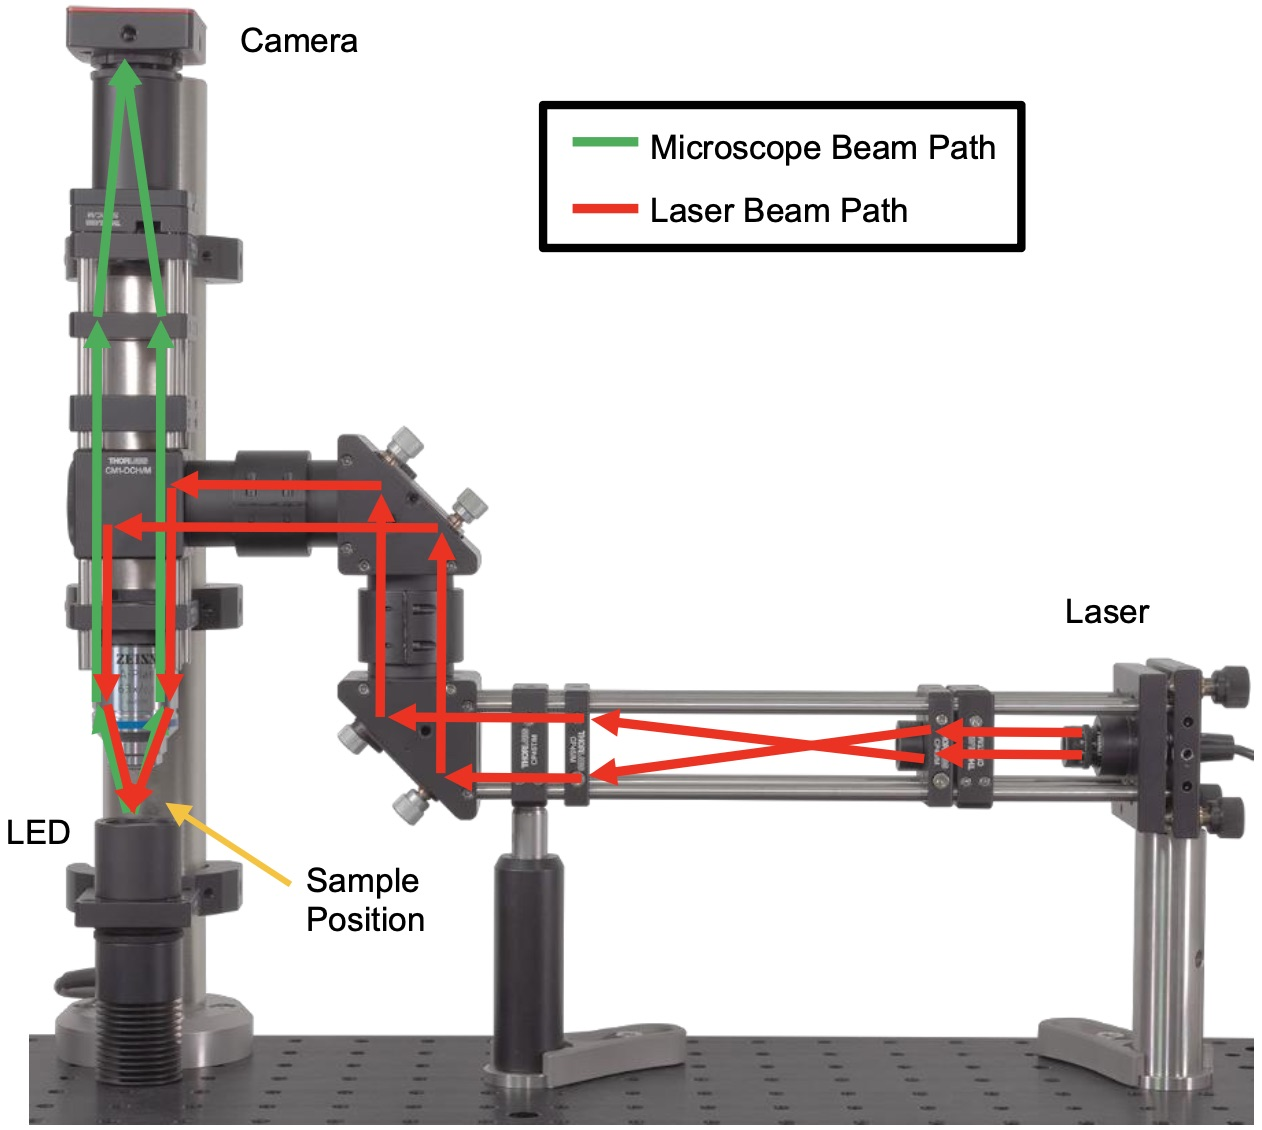
\includegraphics[width=0.7\textwidth]{assets/figures/Introduction/chemin_laser_camera.jpeg}
    \end{center}
    \caption{Trajet du laser et du microscope}
    \label{chemin_laser_caméra}
\end{figure}

La figure ci-dessous (voir Figure \ref{kit_vierge}) correspond au kit reçu lors du premier jour de TB. Le kit a été monté par un assistant du laboratoire COMATEC-LANS.

\begin{figure}[H]
    \begin{center}
        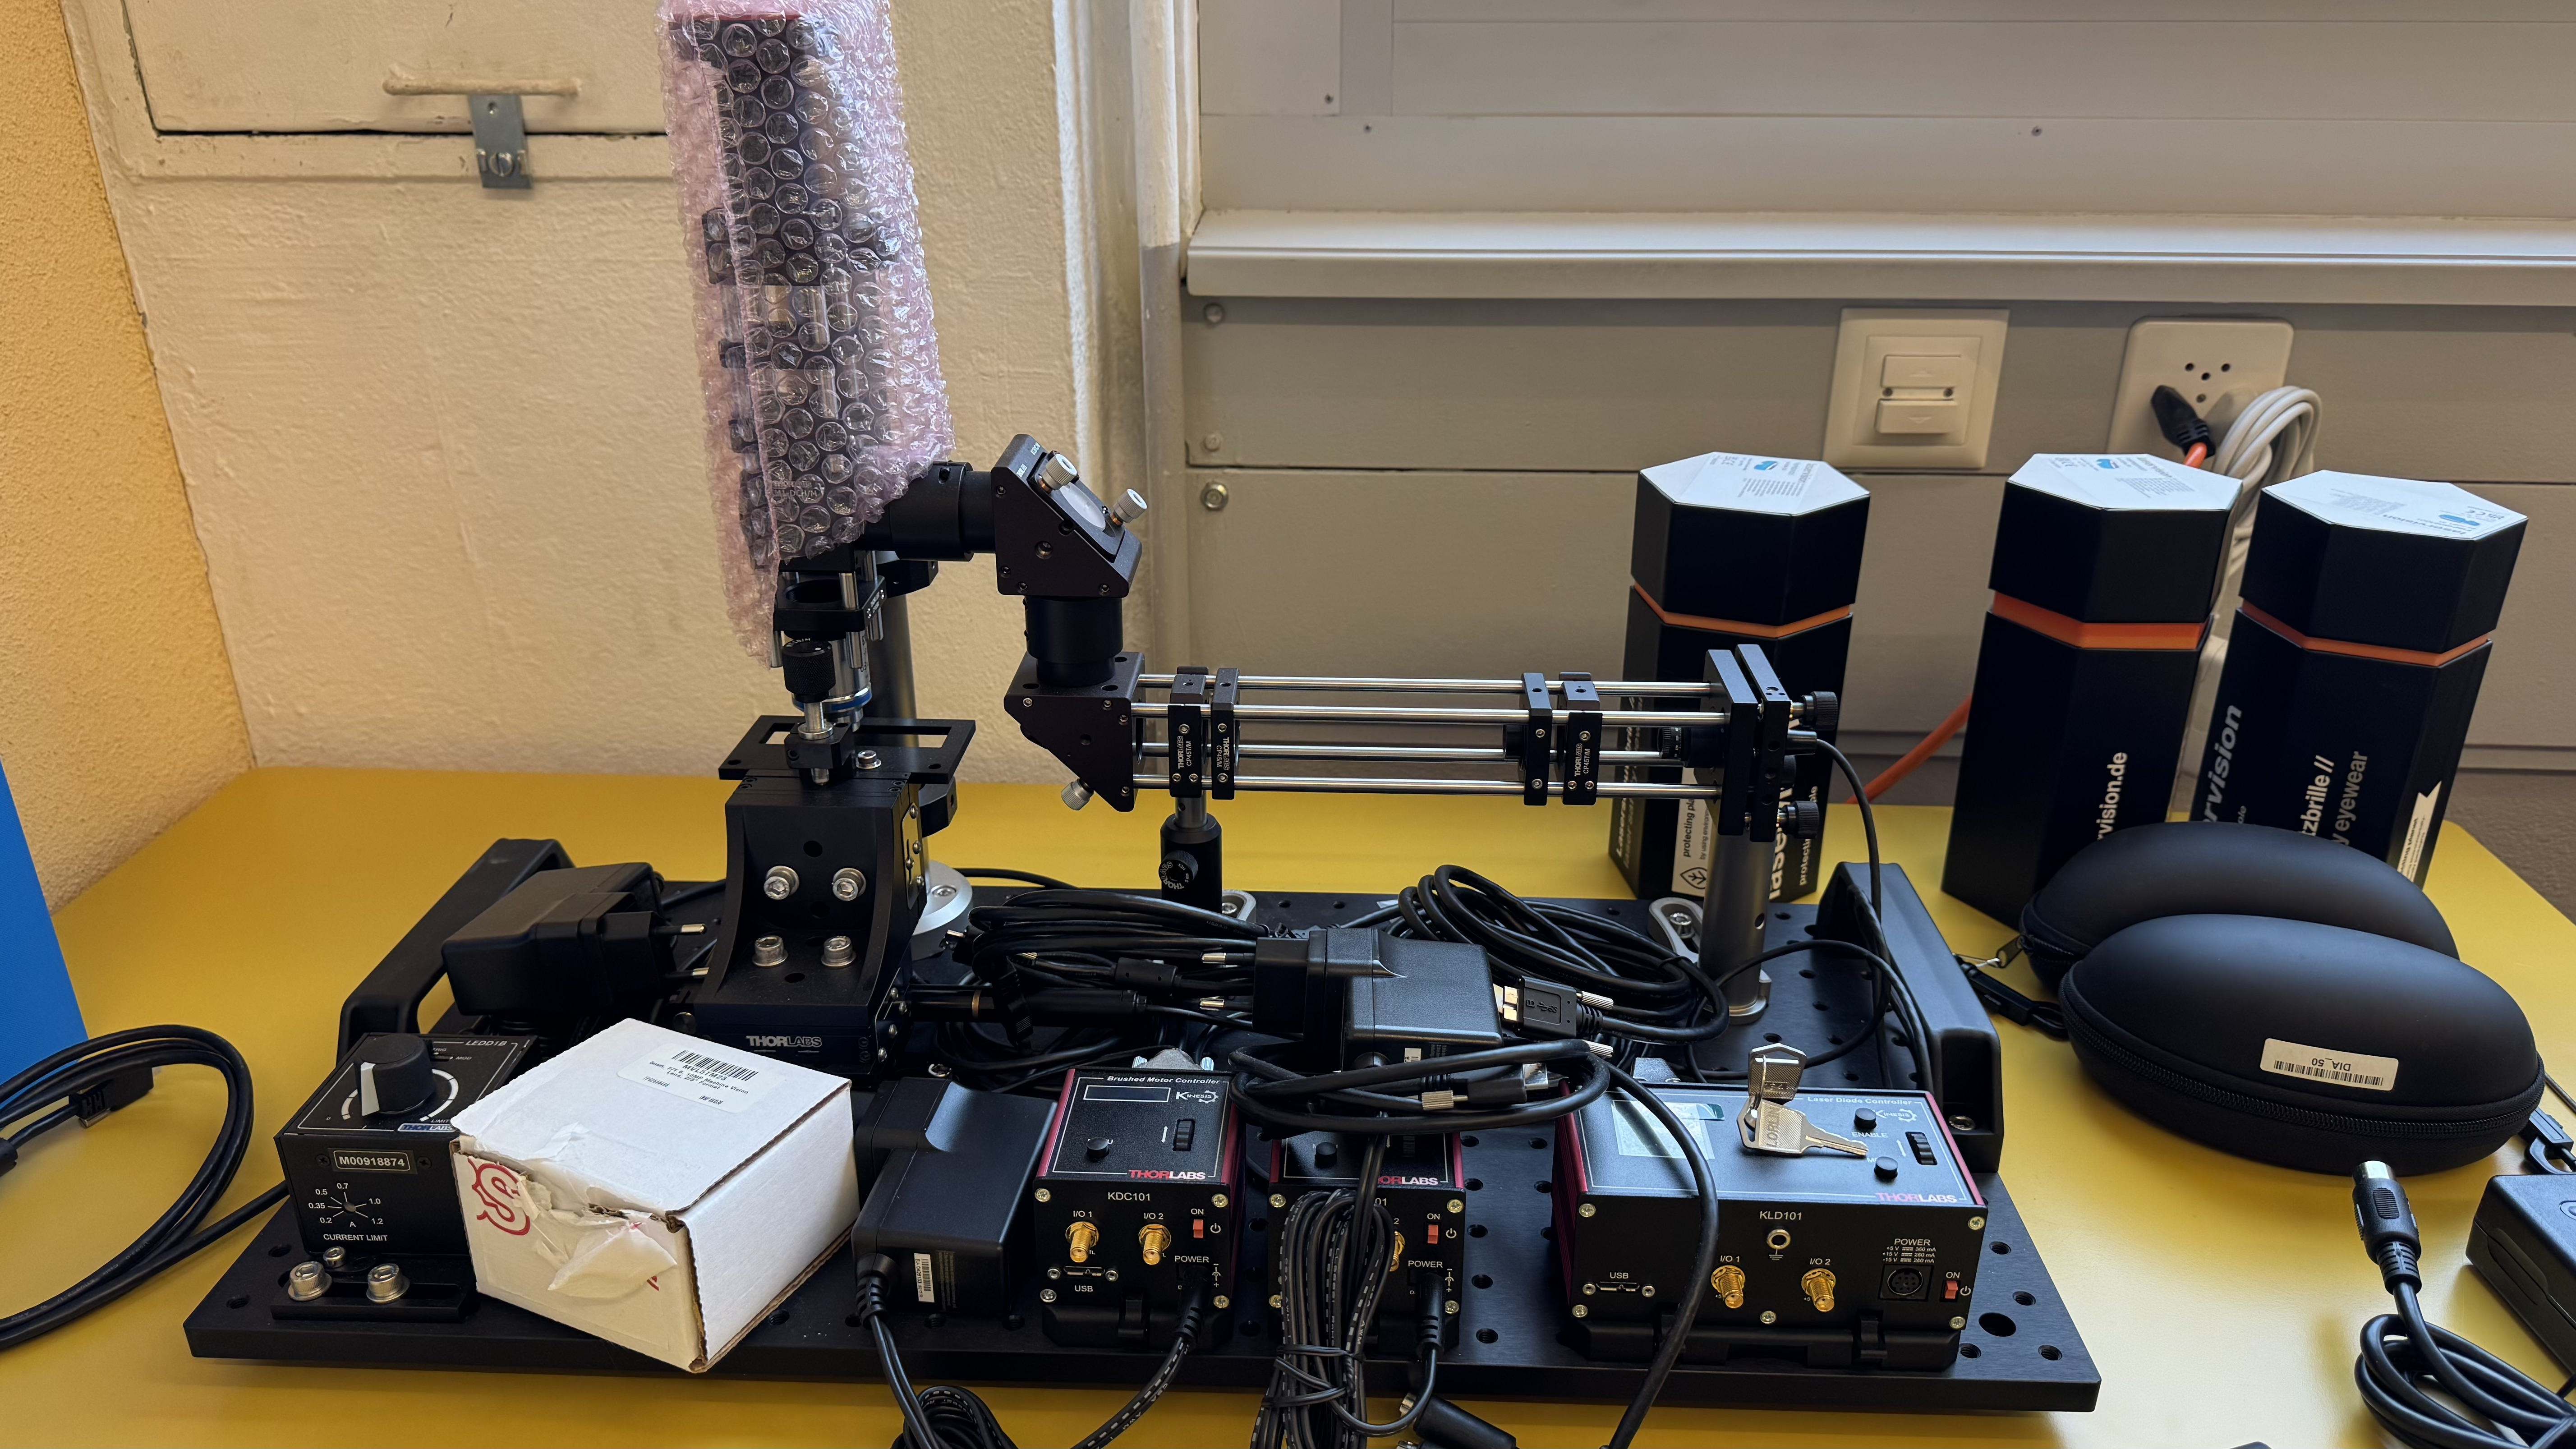
\includegraphics[width=0.7\textwidth]{assets/figures/Introduction/kit_vierge.jpeg}
    \end{center}
    \caption{Kit Portable Optical Tweezers de Thorlabs}
    \label{kit_vierge}
\end{figure}

\newpage
Une représentation 3D du kit, accompagnée de légendes pour chaque composant, a été réalisé par mes soins. Ce modèle CAO permet une clareté et une compréhension plus rapide des différents éléments. Les différentes modélisations 3D des composants ont directement été pris du site Thorlabs \cite{noauthor_portable_nodate}, dans l'onglet \guillemotleft Component List\guillemetright. Je me suis chargé de les rassembler dans un seul fichier CAO et de faire l'assemblage (voir Figure \ref{kit_CAO_vierge_annote}).

\begin{figure}[H]
    \begin{center}
        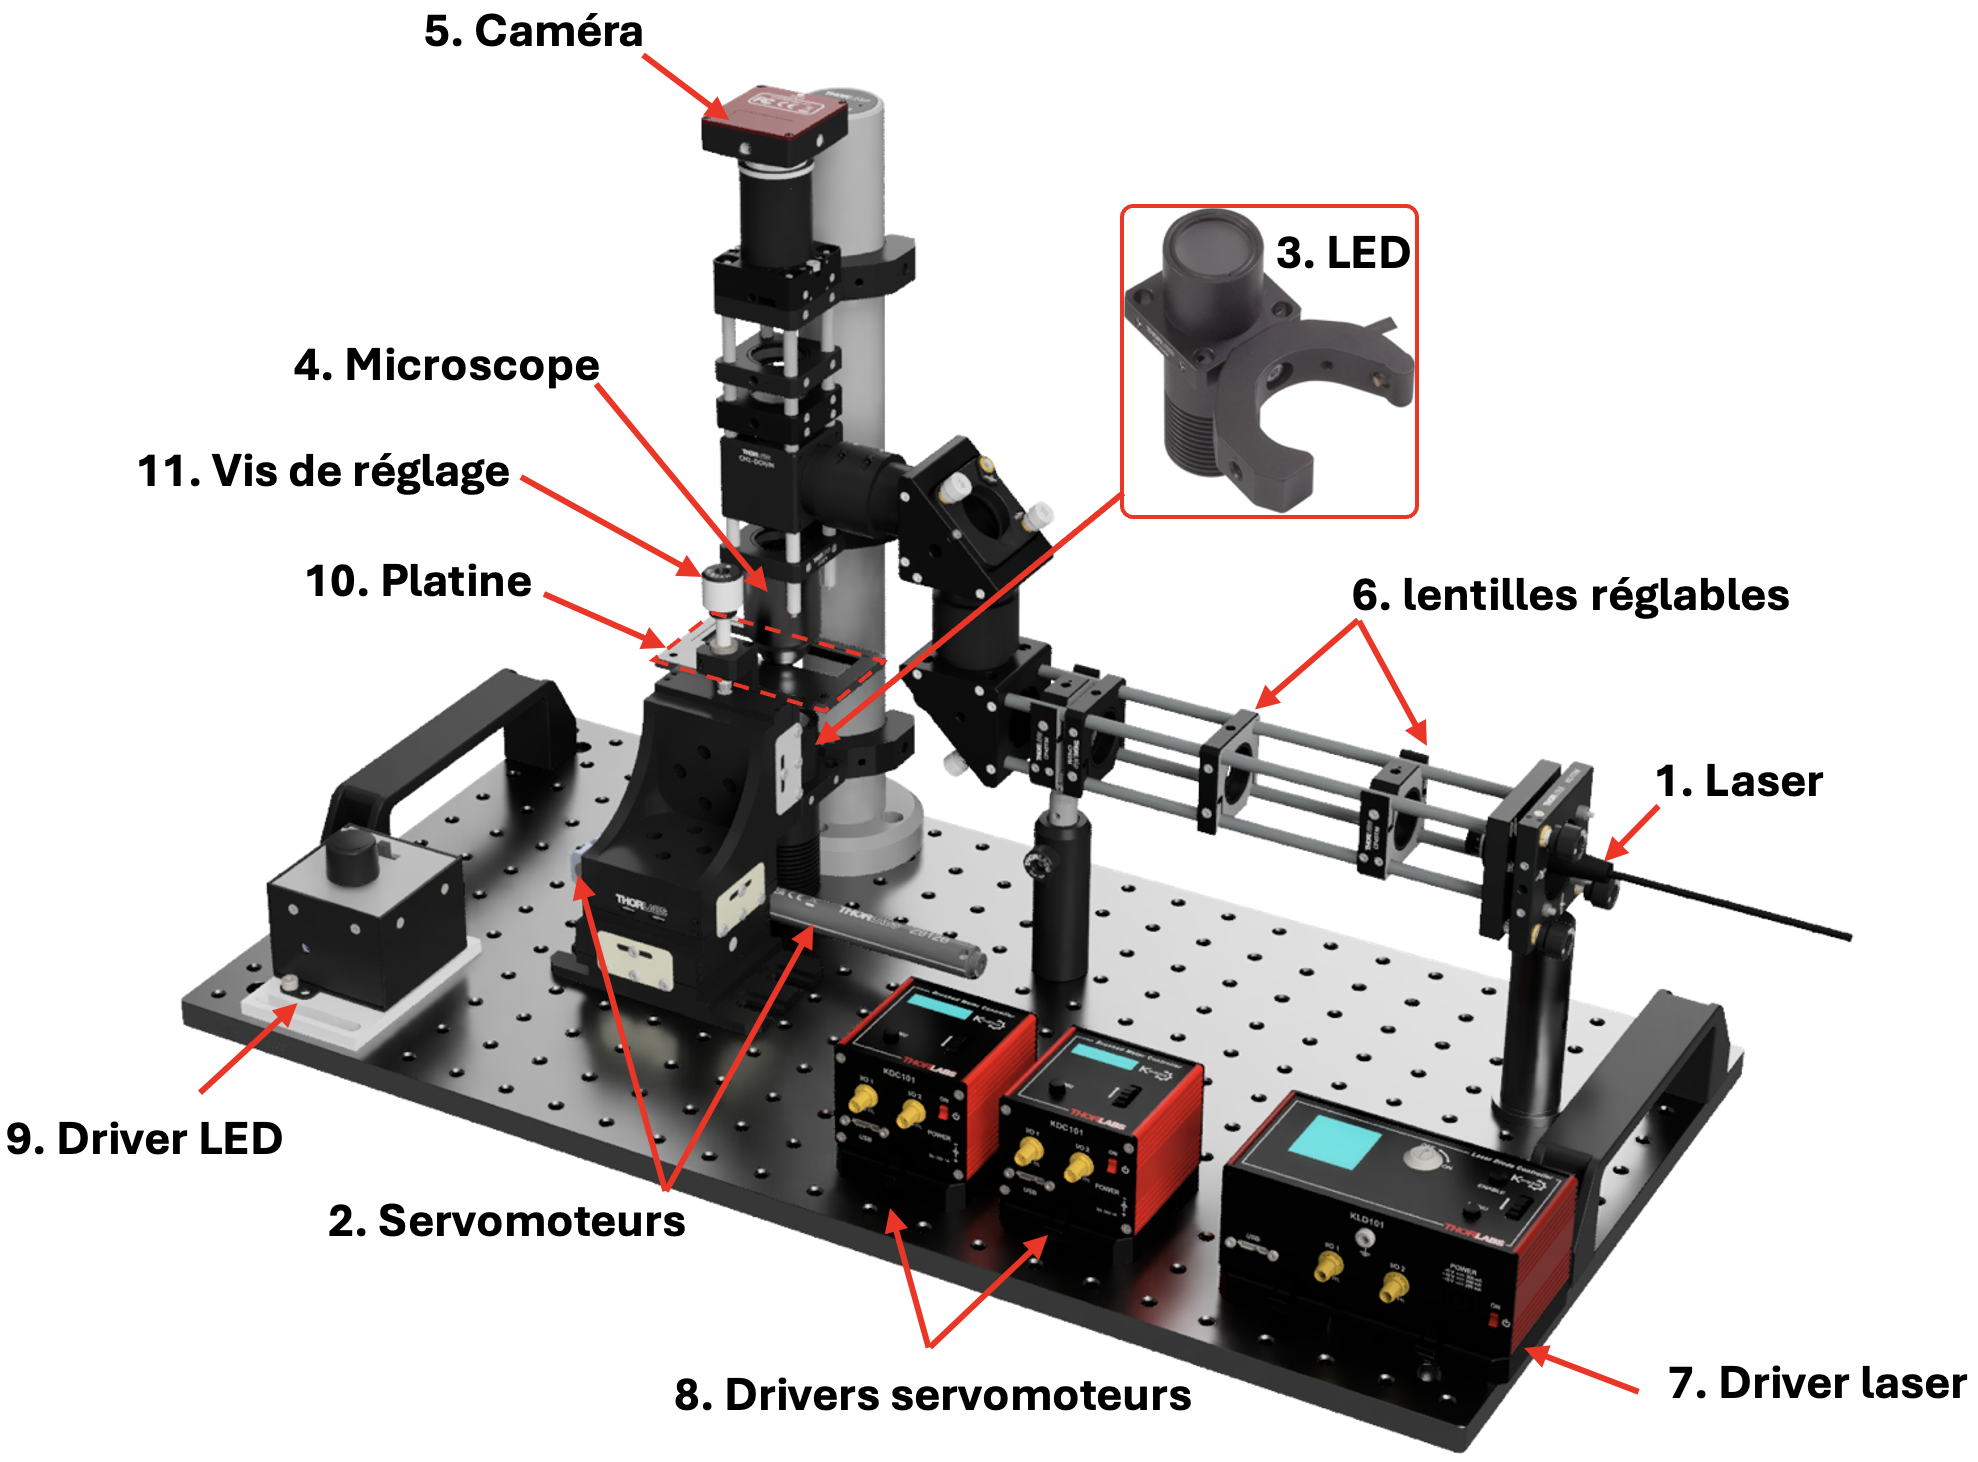
\includegraphics[width=\textwidth]{assets/figures/Introduction/Kit_CAO_vierge_annote.png}
    \end{center}
    \caption{CAO du kit avec annotations des principaux composants}
    \label{kit_CAO_vierge_annote}
\end{figure}

\begin{enumerate}
    \item Laser d'une longueur d'onde 658 nm (couleur rouge visible) avec une puissance maximale de 40 mW.
    \item Les servomoteurs permettent de déplacer la platine en X Y.
    \item La LED permet un réglage manuel de l'éclairage.
    \item Microscope équipé d'un objectif avec un grossissement de $63\times$ et une ouverture numérique de 0,8.
    \item Caméra couleur de 1,6 mégapixel.
    \item Lentilles réglables pour modifier la hauteur de la mise au point du laser.
    \item Ce driver permet de piloter le laser, soit directement avec les boutons intégrés, soit via l'application Kinesis pour une meilleure ergonomie.
    \item Ces driver permettent le pilotage des servomoteurs, soit directement avec les boutons intégrés, soit via l'application Kinesis pour une meilleure ergonomie.
    \item Ce driver permet de faire varier l'intensité lumineuse de la LED.
    \item La platine permet d'accueillir l'échantillon que l'on veut analyser.
    \item La vis de réglage, de pas très fin, permet d'ajuster précisement la hauteur souhaitée de la platine.
\end{enumerate}

\section{Objectifs}

Les différents objectifs de ce travail de bachelor sont listés ci-dessous :
\begin{enumerate}
    \item Mettre en service le kit : câblage, calibration du laser
    \item Conception de protection contre le laser afin d'apporter plus de sécurité lors de l'utilisation du kit
    \item Élaboration d'une notice de laboratoire compacte pour utiliser simplement le kit
    \item Effectuer des tests de déplacements de microbilles dans différents milieux, de différentes viscosités, dans différents types de réservoirs ainsi que de multiples canaux.
    \item Analyses expérimentales des forces de déplacement en fonction de la viscosité des fluides
\end{enumerate}

\subsection{Mise en service du kit}

La première partie consiste à mettre en service le kit. Il faut alimenter les différents drivers qui contrôlent les moteurs, la LED ainsi que le driver pour le laser. Viens ensuite la procédure de calibration du laser, ainsi que l'installation des logiciels permettant de contrôler, d'une part les drivers des moteurs, et d'autre part le driver du laser.
\subsection{Protections contre le laser}
La deuxième partie porte sur la conception des protections contre le laser. Deux parties du kit ont besoin d'avoir une protection totale afin d'éviter toutes reflexions nocives du laser dans les yeux de l'utilisateur. La première protection à réaliser est située au début du laser et va devoir entouré toute la cage oû le laser passe (voir Figure \ref{protection_laser_début}). L'encadré en \textcolor{red}{rouge} représente l'endroit où va devoir être imaginer la protection.

\begin{figure}[H]
    \begin{center}
        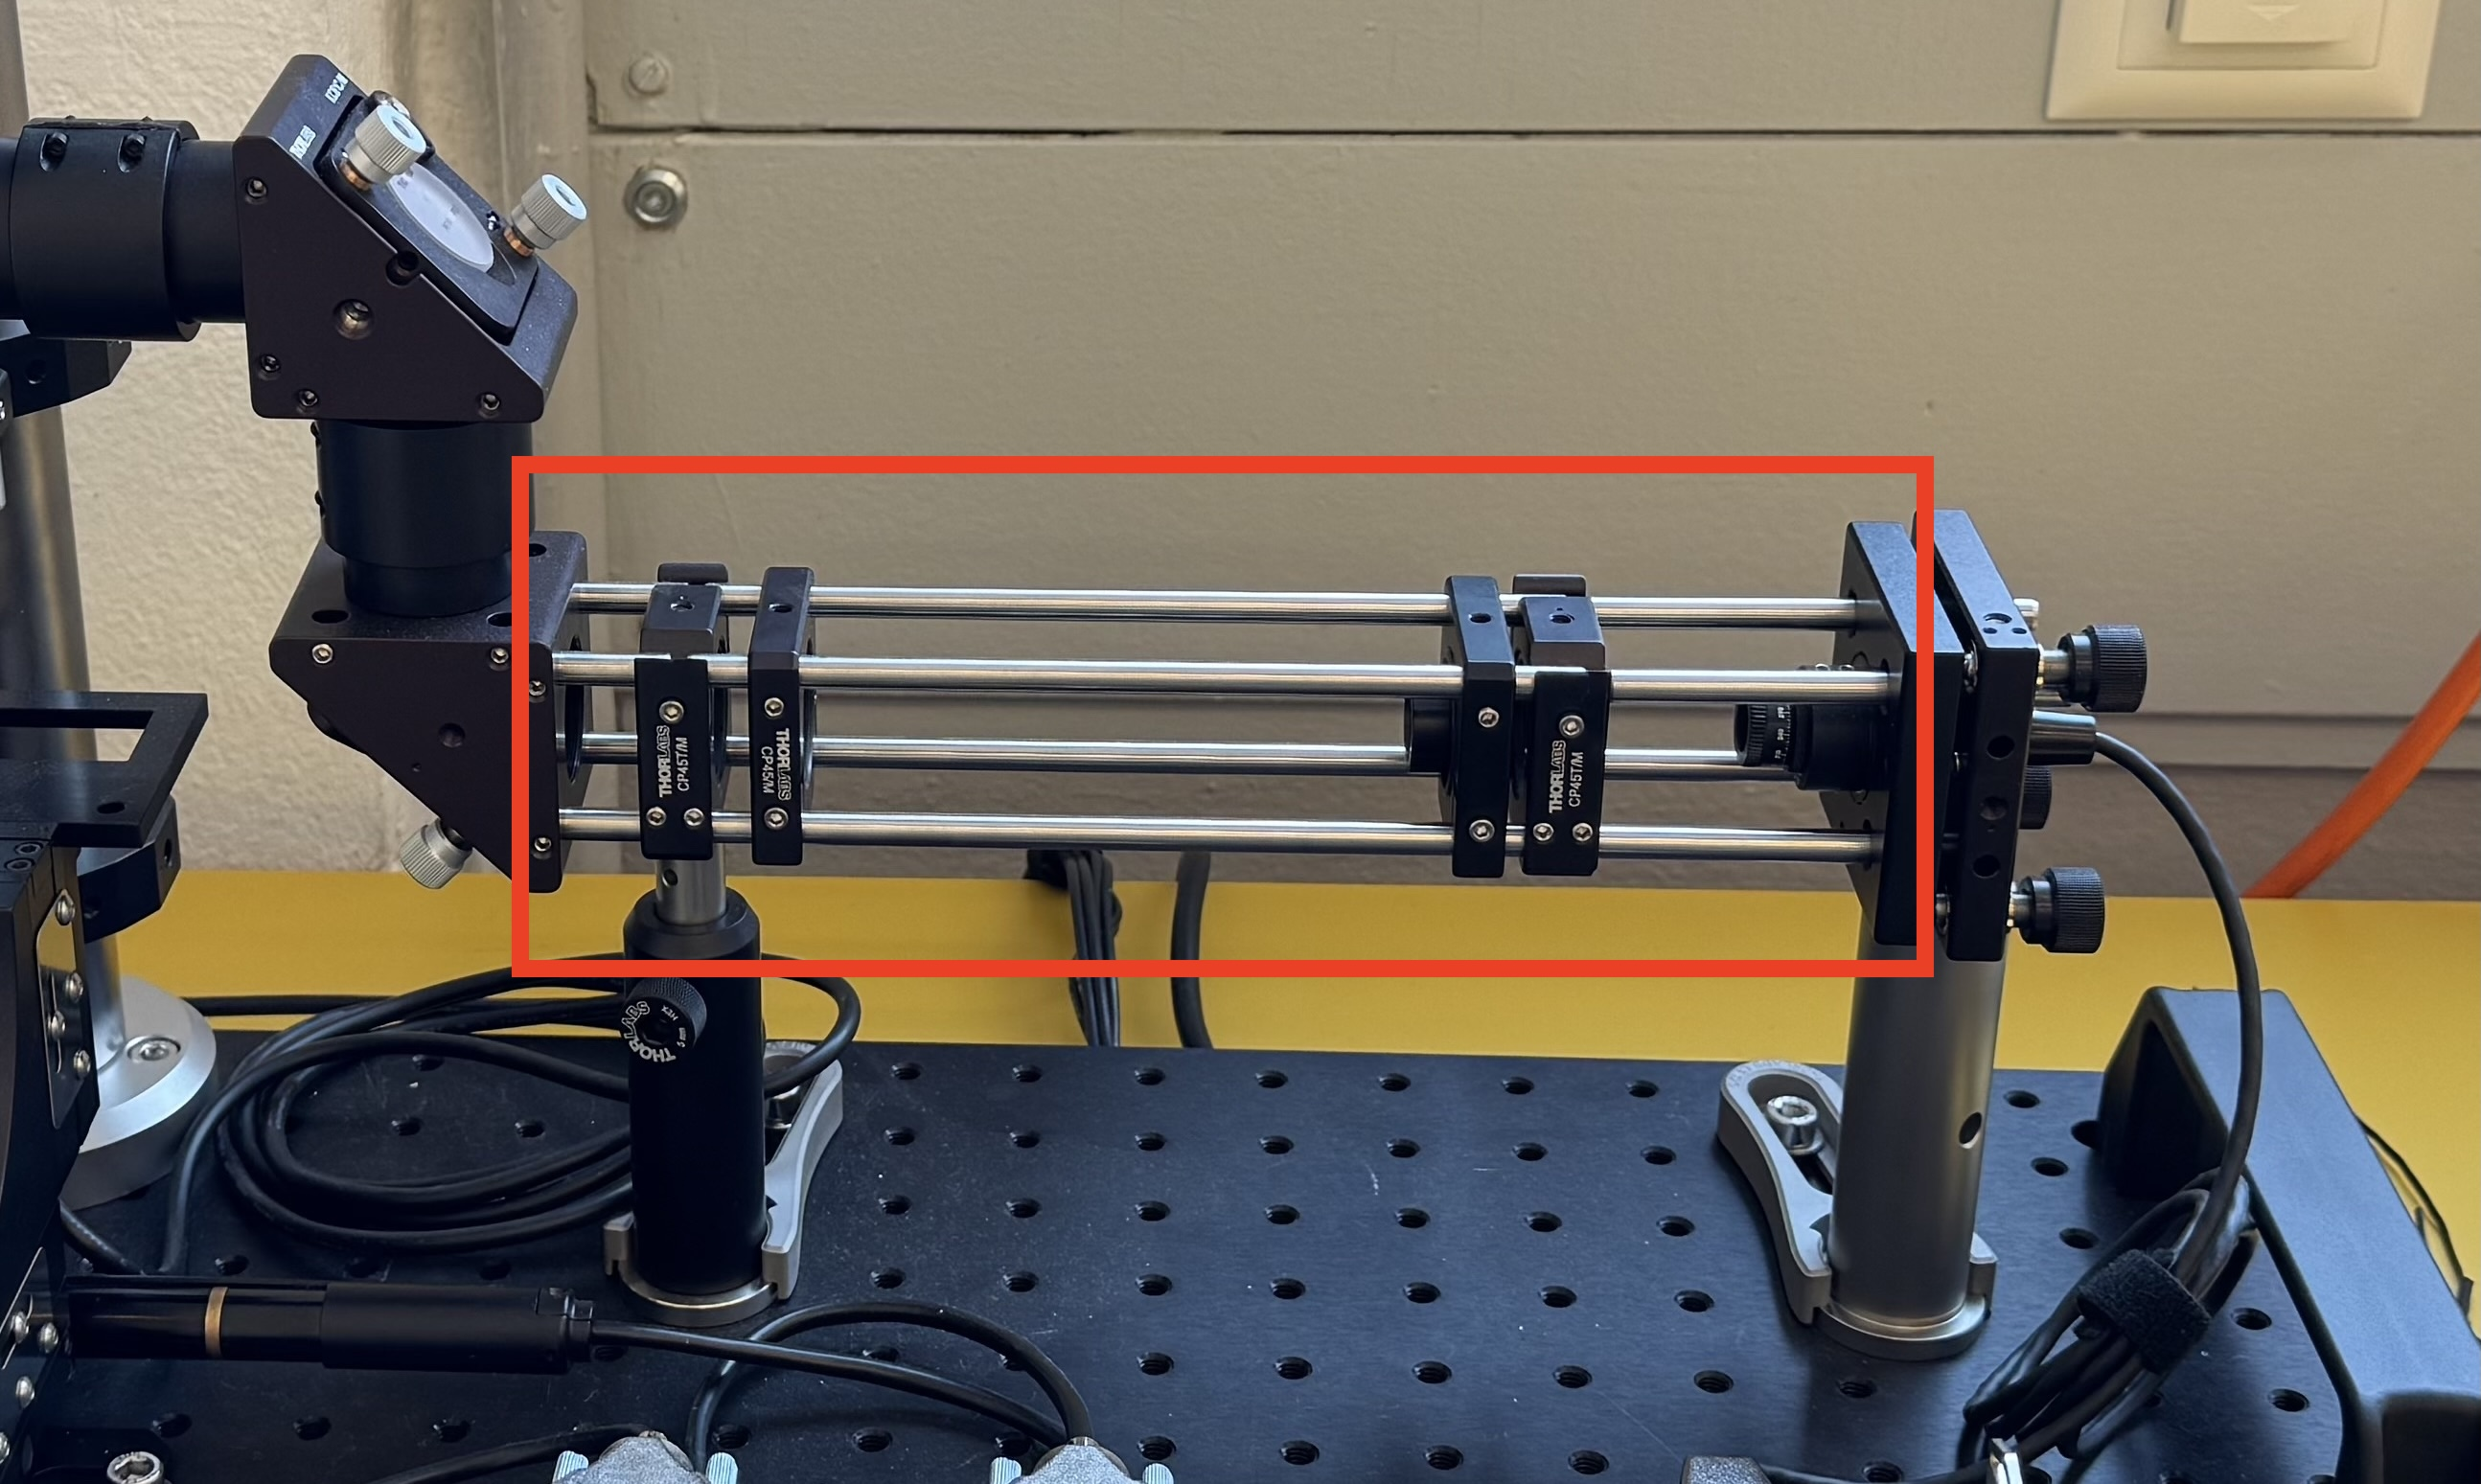
\includegraphics[width=0.5\textwidth]{assets/figures/Introduction/protection_debut_laser.jpeg}
    \end{center}
    \caption{Première protection contre le laser située vers le laser}
    \label{protection_laser_début}
\end{figure}

Une deuxième protection va être faite vers le microscope, car également à cet endroit, le laser devient visible à l'oeil nu et il y'a un grand risque de se blesser. L'encadré en \textcolor{blue}{bleu} représente l'endroit où va devoir être imaginer la protection. Voir la Figure \ref{protection_laser_fin}.

\begin{figure}[H]
    \begin{center}
        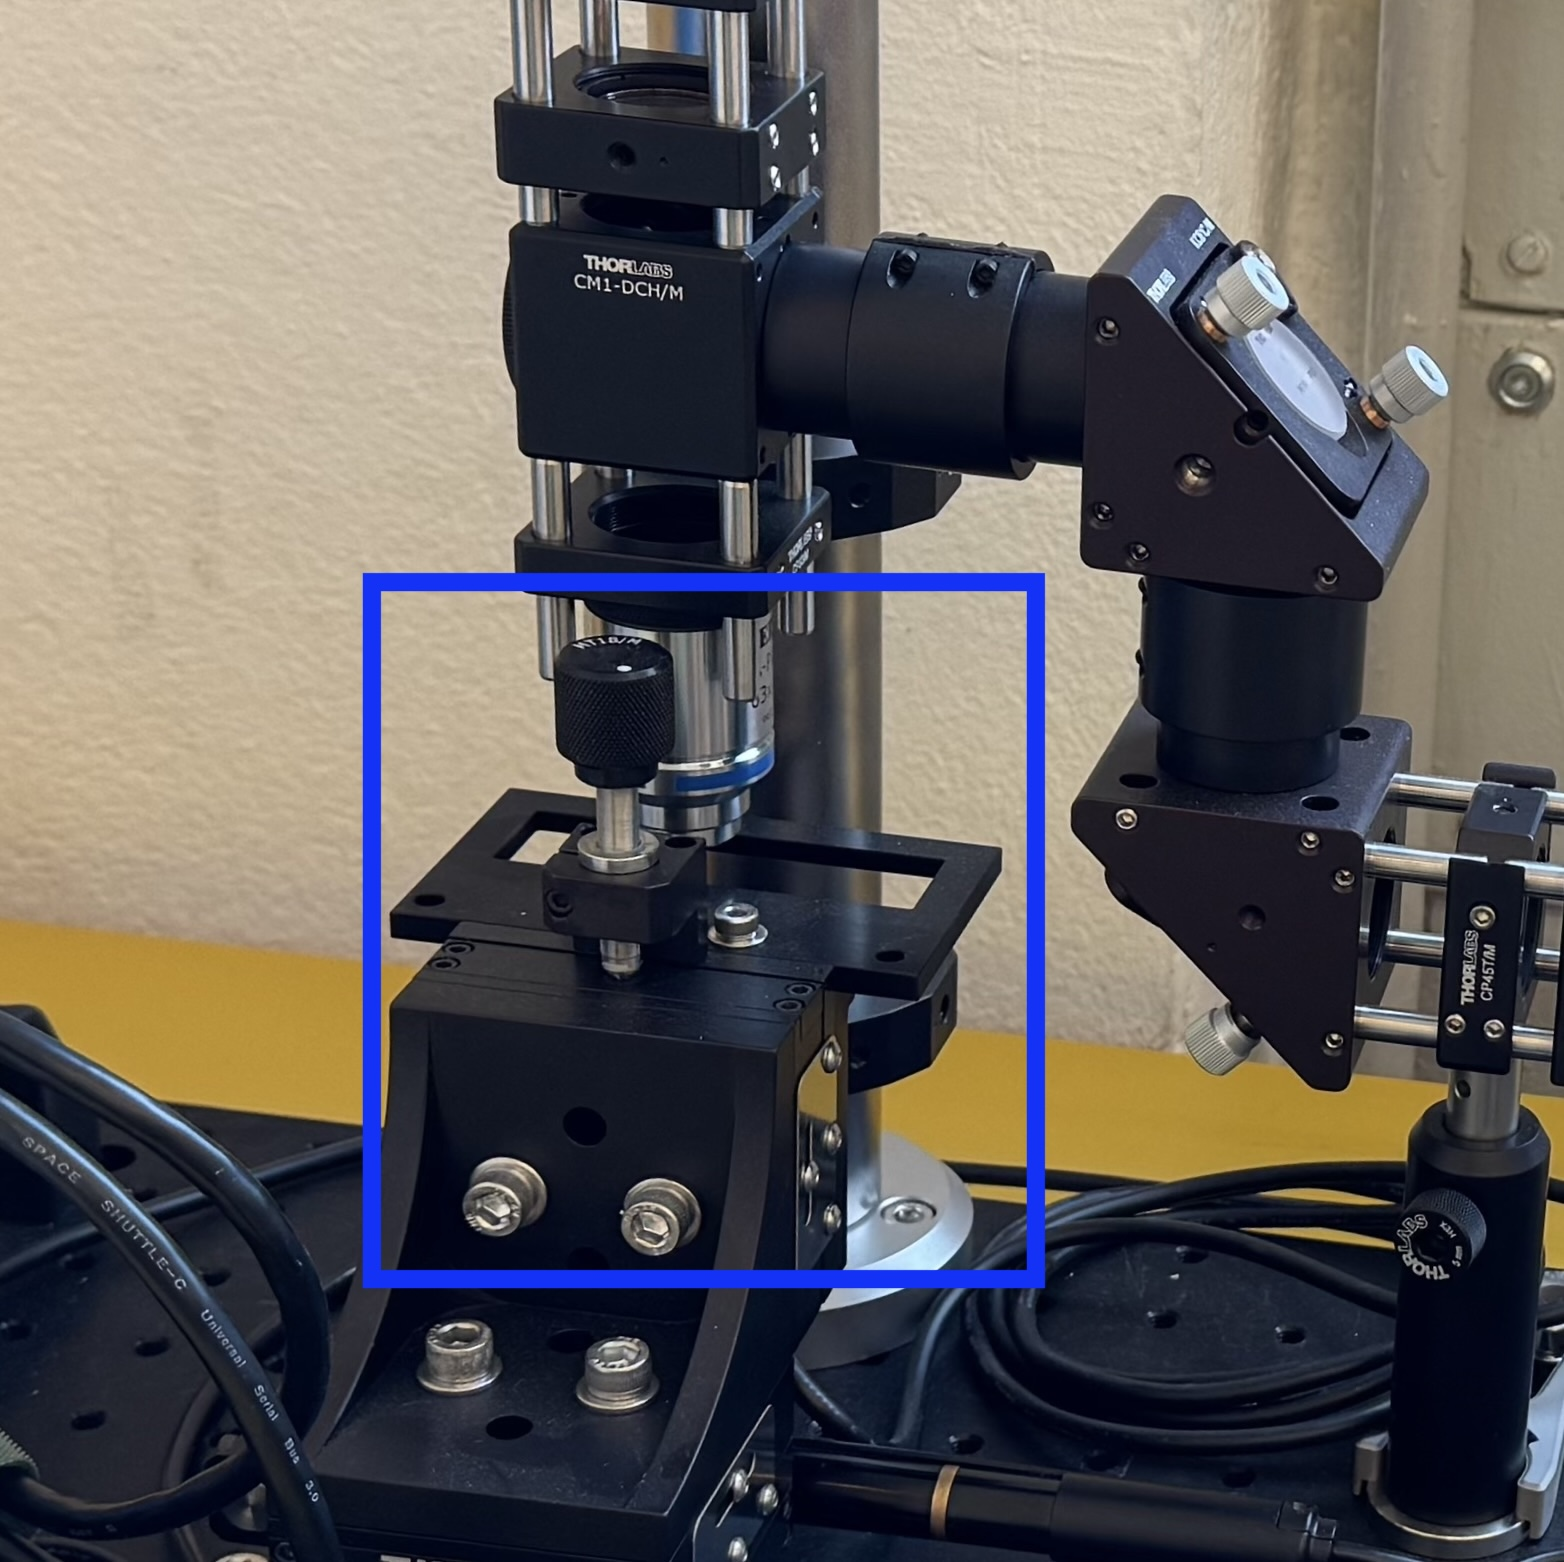
\includegraphics[width=0.5\textwidth]{assets/figures/Introduction/protection_fin_laser.jpeg}
    \end{center}
    \caption{Deuxième protection contre le laser située vers le microscope}
    \label{protection_laser_fin}
\end{figure}

\subsection{Notice de laboratoire}

Un des objectifs de ce TB, consite également à créer une notice de laboratoire pour un cours d'étudiants de la filière système industriels. Cette notice devra être simple à comprendre, compacte et comprendra des manipulations avec différents liquides, ainsi que des mesures pratiques.

%%if
\section{Citations et bibliographie}
Citer vos sources est essentiel. Avec \texttt{biblatex} vous pouvez facilement citer des articles, des livres ou des sites internet. Toutes les citations dans le texte seront automatiquement regroupées en fin de document dans la section \guillemotleft Bibliographie\guillemotright. Par exemple, citons un article d'Einstein \cite{einstein} ou le livre de Dirac \cite{dirac}.

Parfois il peut être utile d'utiliser un gestionnaire de bibliographie. La communauté académique recommande l'outil \href{https://www.zotero.org/}{Zotero} qui permet de gérer une bibliothèque numérique d'ouvrages et de références numériques. Il permet également de générer une bibliographie compatible avec \LaTeX.

Notez qu'il est très facile d'obtenir l'extrait \texttt{bibtex} depuis des journaux. Sélectionnez \emph{export/citation}. Si vous le pouvez choisissez \texttt{bibtex}. Dans le cas d'un format \texttt{.ris}, utilisez un convertisseur en ligne comme \href{http://www.bruot.org/ris2bib/}{ris2bib}.

\section{Adapter votre modèle}
Ce document n'est qu'un modèle ayant pour but de revoir les quelques avantages de \LaTeX~ et les fonctionnalités qui pourraient vous être utiles pour rédiger un rapport académique. N'hésitez pas à supprimer les parties inutiles et à adapter ce modèle à vos besoins.
%%fi
% \input{examples.tex}
\chapter{Câblage du système}
\section{Solution réalisée}
Une étape essentielle dans tout système électrique réside premièrement dans son câblage. Le but est de réaliser un câblage le plus propre et pratique possible. La figure \ref{cablage_kit_pas_annoté} illustre une photo du système sans les annotations afin que le câblage effectué soit plus visible. On retrouve cette même photo sur la Figure~\ref{cablage_kit_annoté} avec les annotations et les explications en détail des différents câbles.
\begin{figure}[H]
    \begin{center}
        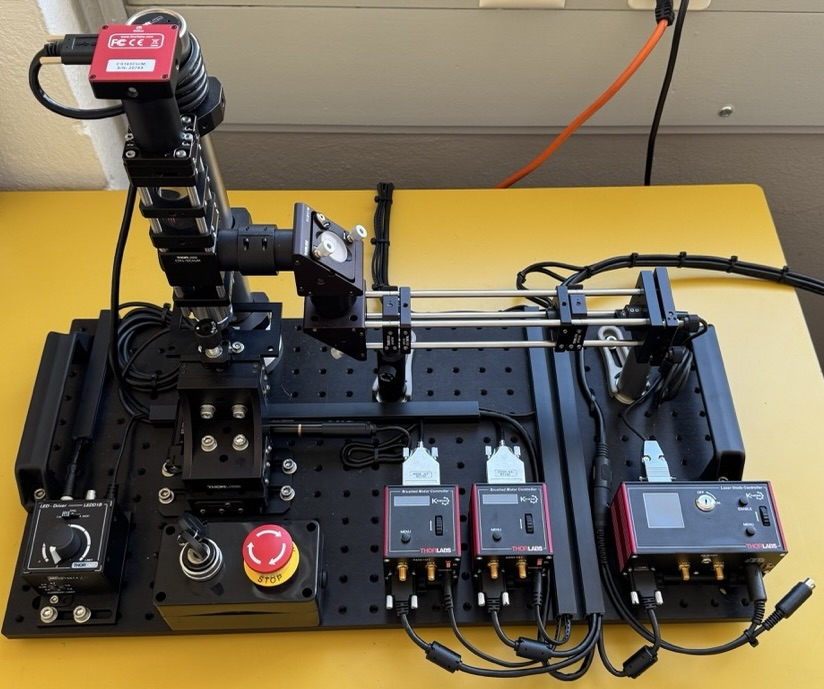
\includegraphics[width=\textwidth]{assets/figures/Cablage_du_kit/Cablage_vierge.jpeg}
    \end{center}
    \caption{Câblage du système sans annotations}
    \label{cablage_kit_pas_annoté}
\end{figure}

\newpage
Une photo du câblage avec des annotations pour une bonne compréhension du travail réalisé est présentée à la Figure \ref{cablage_kit_annoté}.

\begin{figure}[H]
    \centering

    \begin{subfigure}[t]{0.69\textwidth}
        \centering
        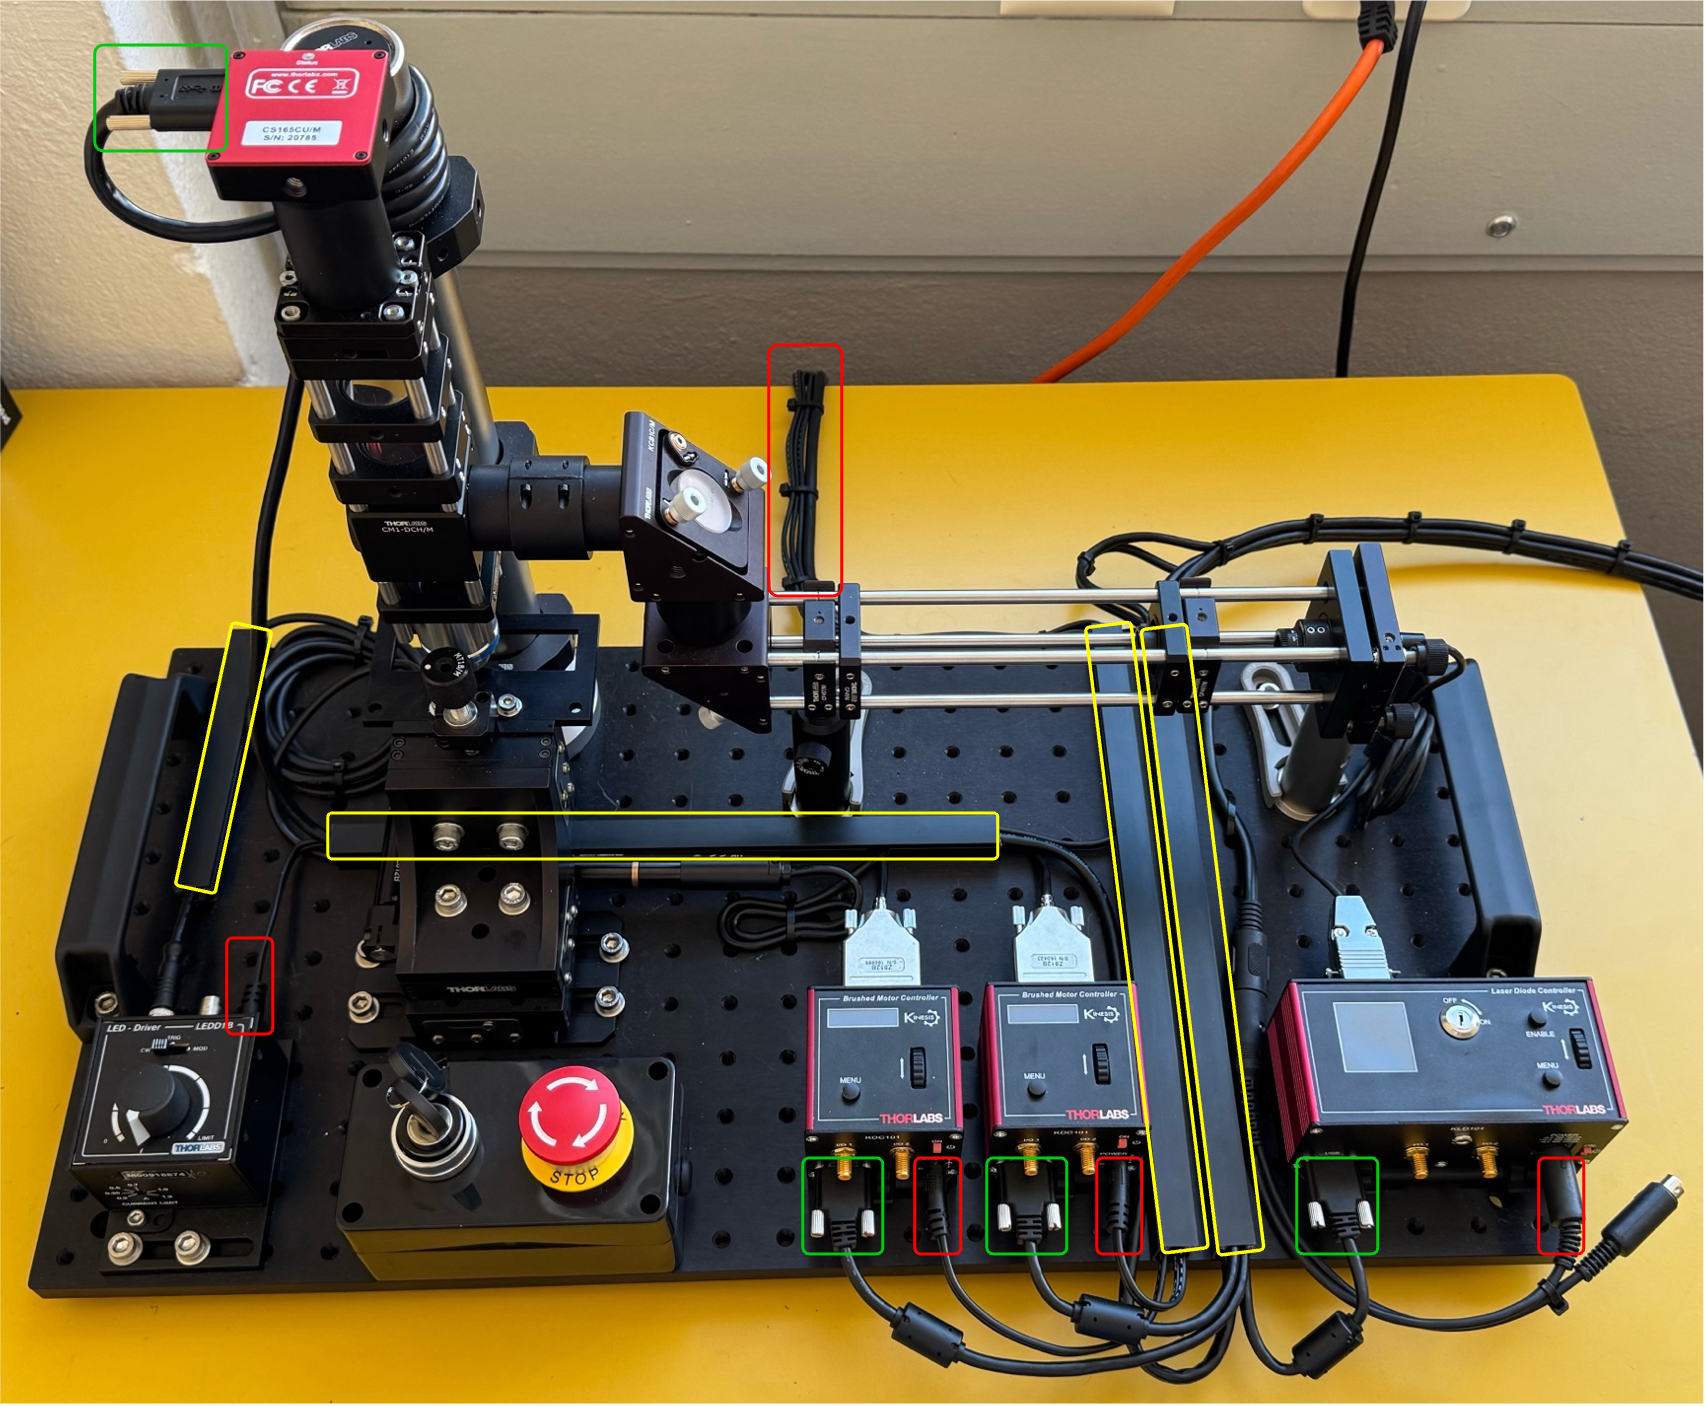
\includegraphics[height=7.9cm]{assets/figures/Cablage_du_kit/cablage_vierge_annote.png}
        \caption{}
        \label{cablage_systeme_complet}
    \end{subfigure}
    \hfill
    \begin{subfigure}[t]{0.29\textwidth}
        \centering
        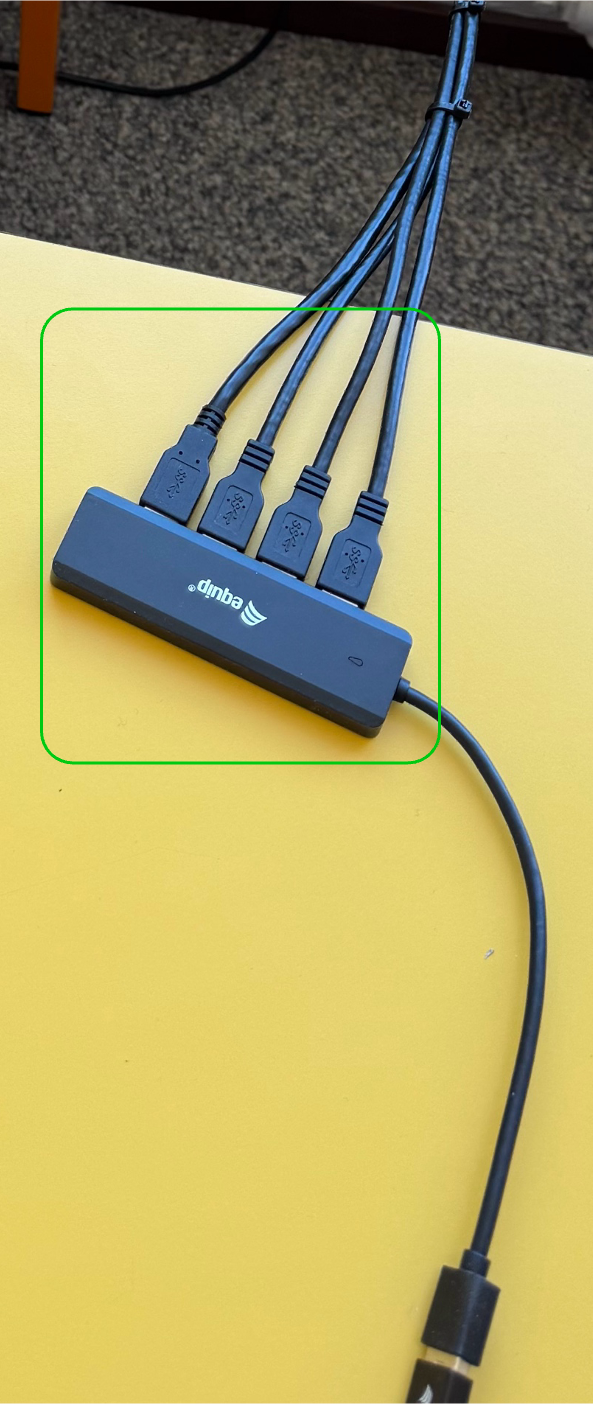
\includegraphics[height=7.9cm]{assets/figures/Cablage_du_kit/Hub_USB_annote.png}
        \caption{}
        \label{cablage_hub_usb}
    \end{subfigure}

    \vskip\baselineskip
    \begin{subfigure}[t]{0.98\textwidth}
        \centering
        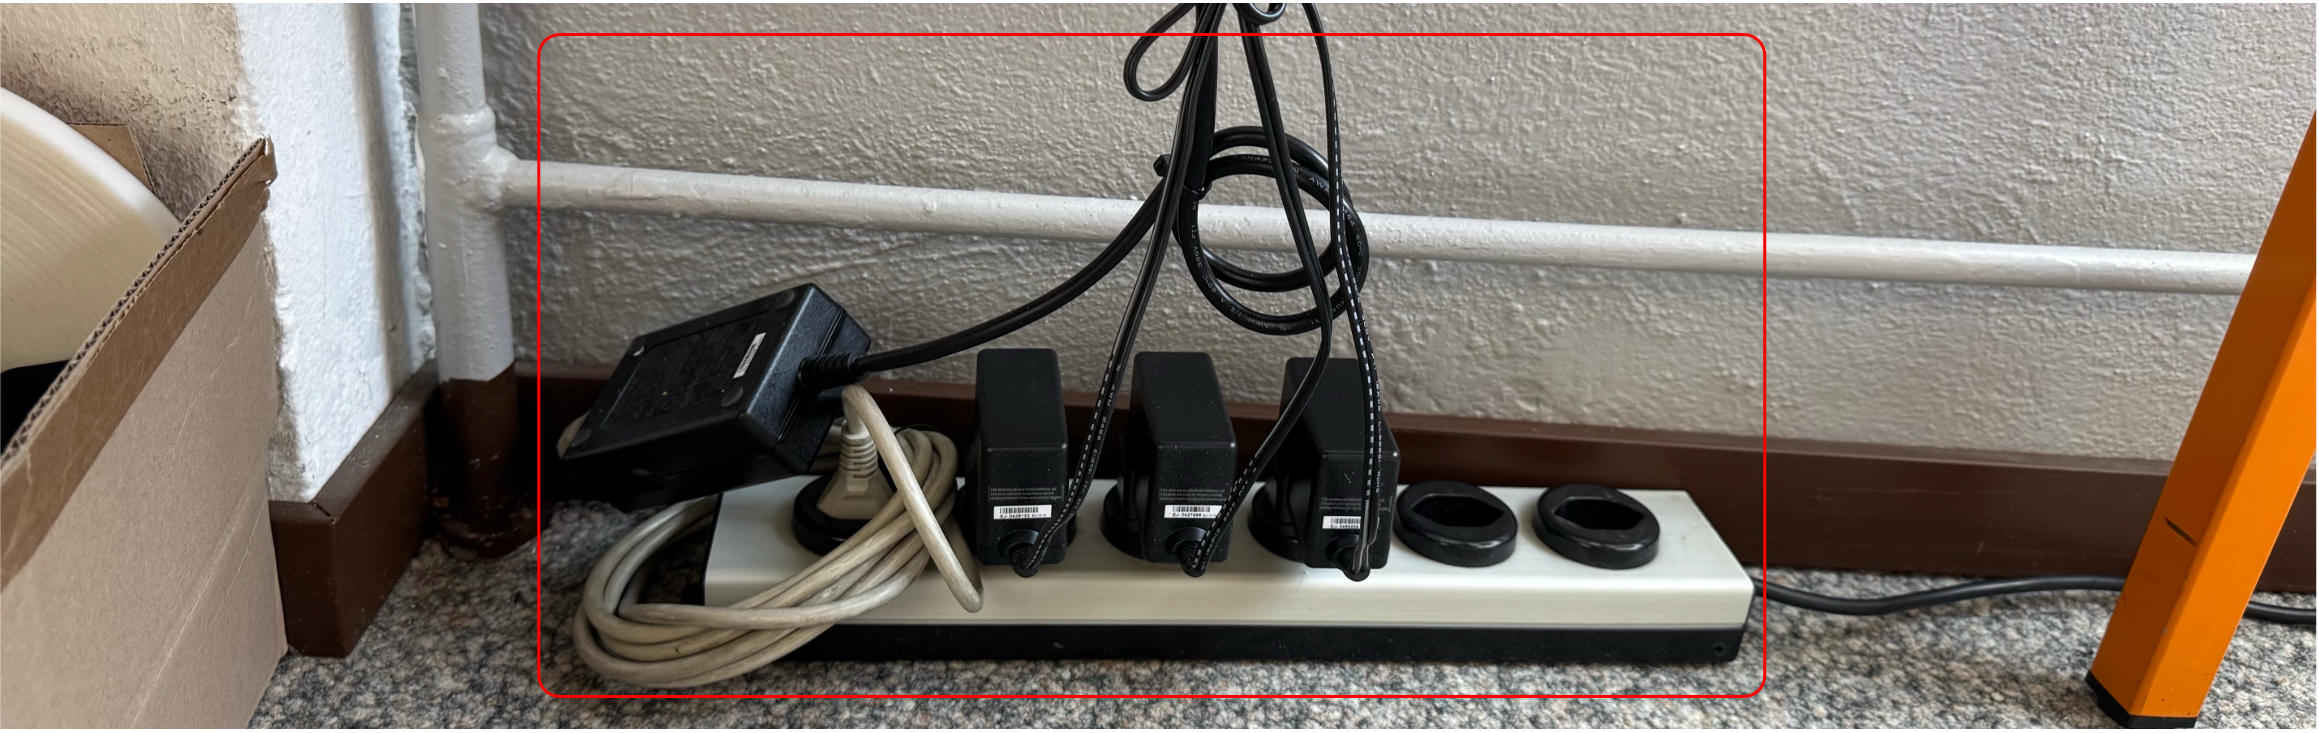
\includegraphics[width=\textwidth]{assets/figures/Cablage_du_kit/Cables_alimentation_annote.png}
        \caption{}
        \label{cablage_alimentation}
    \end{subfigure}

    \caption{Câblage du système avec annotations: a) système complet, b) hub USB-A, c)~alimentations des composants}
    \label{cablage_kit_annoté}
\end{figure}

On peut apercevoir en \textcolor[RGB]{230, 230, 0}{jaune}, que des goulottes ont été installées afin que les câbles tiennent en place, mais également afin d'avoir un visuel au propre.

Les encadrés en \textcolor{red}{rouge} sont les quatres alimentations. Celles-ci sont utilisées pour :
\begin{itemize}
    \item Les deux drivers des servomoteurs
    \item Le driver du laser
    \item Le driver de la LED
\end{itemize}
\vspace{0.5em}
En complément des alimentations, les encadrés en \textcolor[RGB]{0, 201, 18}{vert} désignent les câbles permettant de communiquer avec les différents composants. Voici, ci-dessous, la liste des câbles pour la communication :
\begin{itemize}
    \item Un câble pour chaque driver de servomoteur, deux au total
    \item Un câble pour le driver du laser
    \item Un câble pour la caméra
\end{itemize}
\vspace{0.5em}
Tous les câbles de communications sont connectés à un hub USB-A, voir la Figure~\ref{cablage_hub_usb}, afin d'avoir en sortie plus qu'un seul câble à brancher au PC.

\chapter{Sécurité électrique} \label{chapter:securite_electrique}
Pour une sécurité optimale, il est judicieux d'ajouter, en plus des protections mécaniques, des capteurs afin de détecter si une protection est ouverte.

Afin de renforcer la sécurité, un arrêt d'urgence ainsi qu'une clé de maintenance seront ajoutés. Ces deux capteurs seront reliés et connectés à l'interlock du driver du laser.

\section{Interlock: Principe de fonctionnement}

\begin{minipage}[c]{0.6\textwidth}
    Le driver du laser intègre un système d'interlock permettant de désactiver, si le circuit électrique interlock est ouvert, l'alimentation du laser. Par défaut, un pont est soudé entre les pins 1 et 5, voir la Figure~\ref{No_interlock} ci-contre.
\end{minipage}\hfill
\begin{minipage}[c]{0.35\textwidth}
    \begin{figure}[H]
        \begin{center}
            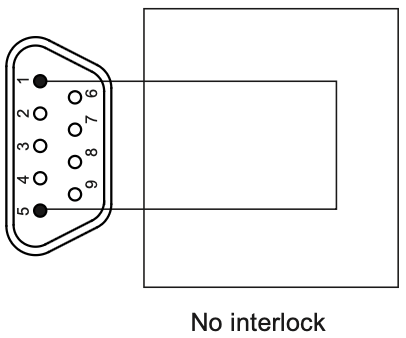
\includegraphics[width=0.8\textwidth]{assets/figures/Protections_laser/Securite_electrique/no_interlock.png}
        \end{center}
        \captionof{figure}{Schéma électrique sans interlock~\cite{LaserDriverKLD101}}
        \label{No_interlock}
    \end{figure}
\end{minipage}
\begin{minipage}[c]{0.6\textwidth}
    L'objectif est d'ajouter un circuit électrique personalisé qui intègre l'interlock. De ce fait, le schéma suivant sera utilisé pour la conception du circuit électrique. Voir la Figure~\ref{Interlock_only}, ci-contre.
\end{minipage}\hfill
\begin{minipage}[c]{0.35\textwidth}
    \begin{figure}[H]
        \begin{center}
            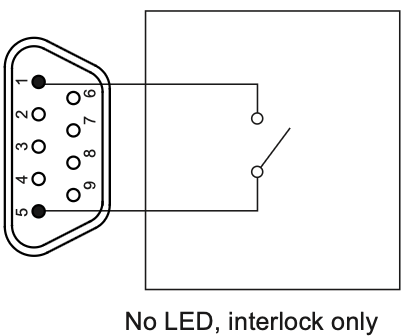
\includegraphics[width=0.8\textwidth]{assets/figures/Protections_laser/Securite_electrique/interlock_only.png}
        \end{center}
        \captionof{figure}{Schéma électrique avec interlock~\cite{LaserDriverKLD101}}
        \label{Interlock_only}
    \end{figure}
\end{minipage}

\newpage
\section{Première version du schéma électrique de l'interlock}
La Figure~\ref{schema_interlock_v1} ci-dessous montre la première version du schéma électrique complet de l'interlock. Comme le choix des capteurs n'est pas encore fait à ce jour, des fins de course ont été représentés de façon provisoire, afin d'avoir une première représentation fonctionnelle du système. L'arrêt d'urgence ainsi que la clé de maintenance seront expliqués à la section~\ref{subsec:arret_urgence_maintenance}.

\begin{figure}[H]
    \begin{center}
        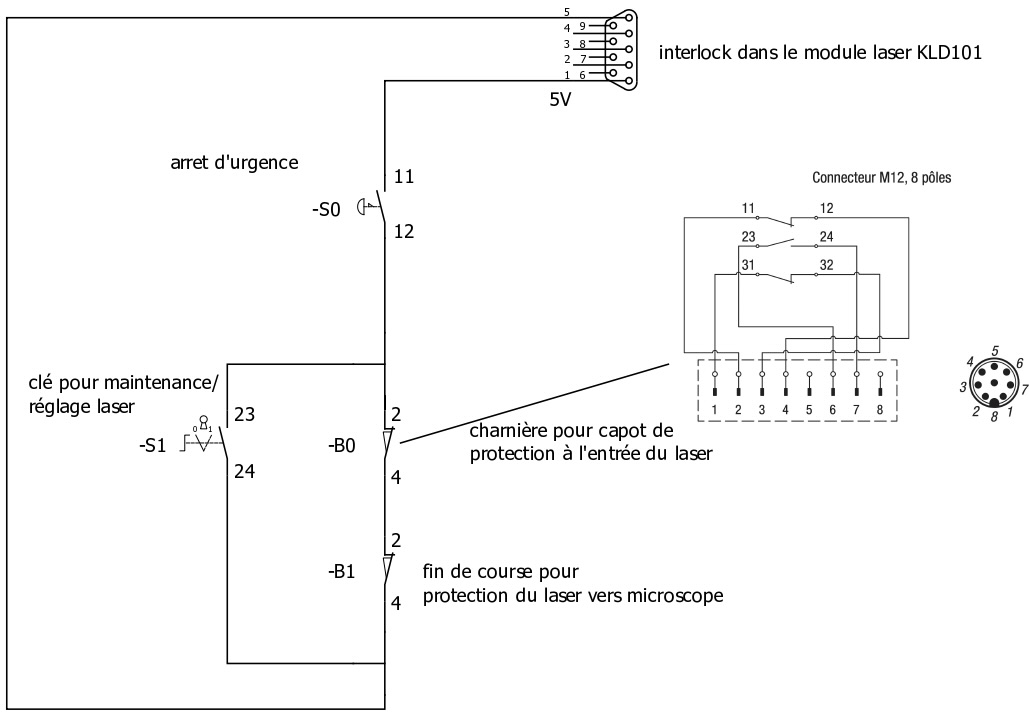
\includegraphics[width=\textwidth]{assets/figures/Protections_laser/Securite_electrique/interlock_schema_elec_V1.jpeg}
    \end{center}
    \caption{Première version du schéma électrique complet de l'interlock}
    \label{schema_interlock_v1}
\end{figure}
\newpage
\section{Capteurs sur les protections mécaniques}
Afin de garantir la sécurité lors de l'utilisation du laser, il est essentiel d'être averti si l'une des deux protections est ouverte.

\subsection{Solutions disponibles sur le marché}
\begin{minipage}[c]{0.6\textwidth}
    Une première recherche s'est portée sur des interrupteurs de sécurité avec vérouillage électrique, que l'on retrouve beaucoup dans l'industrie. Ci-contre, un exemple de ce type d'interrupteur, voir Figure~\ref{interrupteur_telemecanique}.

    Ces serrures ont l'avantage d'être vérouillées électriquement, ce qui permet d'assurer un vérouillage mécanique. Malheureusement, ce type de sécurité est trop volumineux pour notre système.
\end{minipage}\hfill
\begin{minipage}[c]{0.35\textwidth}
    \begin{center}
        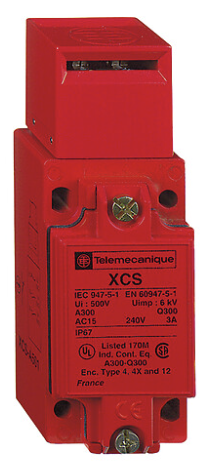
\includegraphics[width=0.45\textwidth]{assets/figures/Protections_laser/Securite_electrique/serrure_telemecanique.png}
    \end{center}
    \captionof{figure}{Interrupteur de sécurité Telemecanique~\cite{interrupteurTelemecanique}}
    \label{interrupteur_telemecanique}
\end{minipage}

\begin{minipage}[c]{0.6\textwidth}
    Le constructeur d'organes de sécurité Pilz propose une charnière comprenant un capteur intégré, qui permet de régler librement le point de commutation du contact entre 0\textdegree{} et 270\textdegree{}.

    Une photo ci-contre montre ce type de charnière électrique, voir Figure~\ref{charniere_pilz}.
\end{minipage}\hfill
\begin{minipage}[c]{0.35\textwidth}
    \begin{center}
        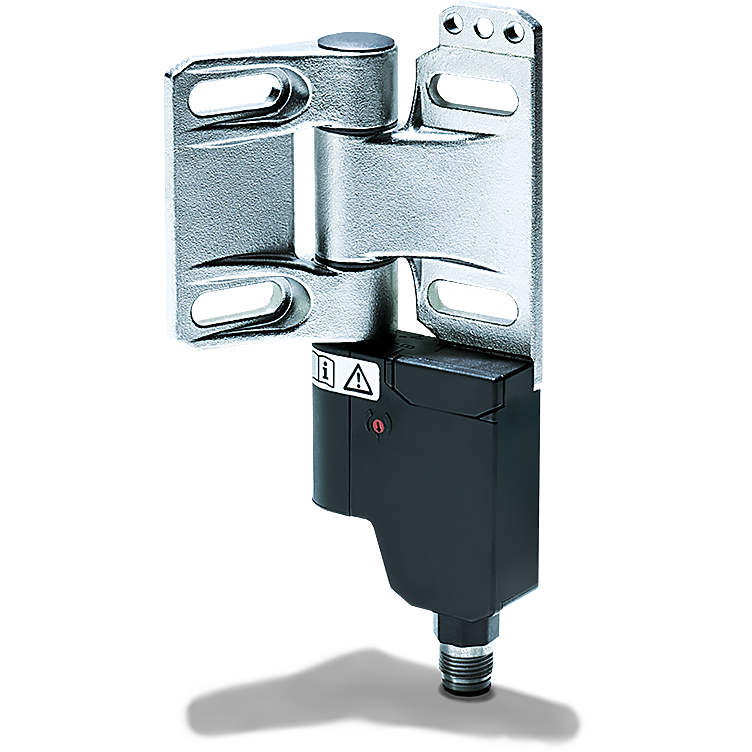
\includegraphics[width=0.6\textwidth]{assets/figures/Protections_laser/Securite_electrique/charniere_pilz.png}
    \end{center}
    \captionof{figure}{Charnière de sécurité Pilz~\cite{charnierePilz}}
    \label{charniere_pilz}
\end{minipage}

\begin{minipage}[c]{0.6\textwidth}
    Une dernière option de charnière de sécurité a été élaborée par l'entreprise Norelem. Avec cette charnière, on peut également régler l'angle de commutation. L'avantage de celle-ci est que le capteur est directement intégré dans la charnière, le rendant totalement invisible.

    Ci-contre, une photo de la charnière de Norelem, voir Figure~\ref{charniere_norelem}.
\end{minipage}\hfill
\begin{minipage}[c]{0.35\textwidth}
    \begin{center}
        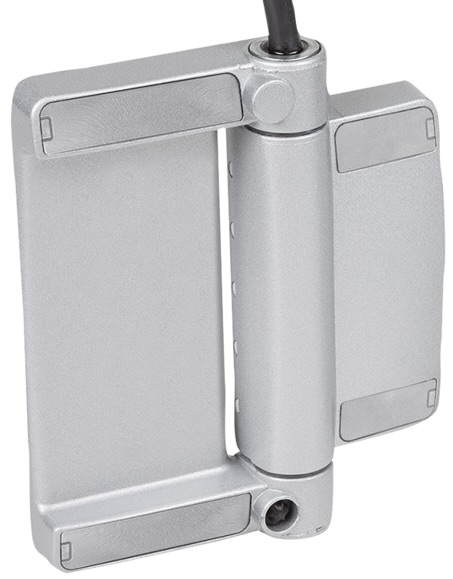
\includegraphics[width=0.75\textwidth]{assets/figures/Protections_laser/Securite_electrique/charniere_norelem.jpeg}
    \end{center}
    \captionof{figure}{Charnière de sécurité Norelem~\cite{charniereNorelem}}
    \label{charniere_norelem}
\end{minipage}

\begin{minipage}[c]{0.6\textwidth}
    Le fin de course est souvent utilisé en électronique, car il ne prend pas beaucoup de place et il est facile à implémenter. Bien que cette solution soit discrète, cela reste un système de sécurité simple, et peut être facilement contourné.

    Ci-contre, une photo du fin de course, voir Figure~\ref{fin_de_course}.
\end{minipage}\hfill
\begin{minipage}[c]{0.35\textwidth}
    \begin{center}
        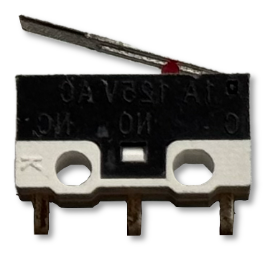
\includegraphics[width=0.6\textwidth]{assets/figures/Protections_laser/Securite_electrique/fin_de_course.png}
    \end{center}
    \captionof{figure}{Fin de course}
    \label{fin_de_course}
\end{minipage}

\newpage
\subsection{Solution choisie pour la protection à l'entrée du laser}
La solution finale pour cette protection s'est tournée sur la charnière de sécurité de l'entreprise Norelem. Elle contient tous les avantages que l'on recherche pour ce travail :
\begin{itemize}
    \item Elle s'intègre dans la conception de la protection, car il est nécessaire d'avoir une charnière pour soulever celle-ci.
    \item Elle contient un capteur de position intégré.
    \item L'angle de commutation est réglable.
    \item Elle est compacte, ce qui facilite son intégration dans le kit actuel.
    \item Il s'agit d'une solution robuste, conçue pour un usage industriel, ce qui assurera son efficacité dans le temps.
\end{itemize}

\subsection{Solution choisie pour la protection vers le microscope}
La solution finale pour cette protection s'est tournée sur le fin de course. Ses avantages :
\begin{itemize}
    \item Il n'y a pas beaucoup de place vers le microscope pour faire une protection, par conséquent, sa taille permet d'être installée presque où l'on souhaite.
    \item Il est peu coûteux et facilement remplaçable.
    \item Malgré sa sécurité simple, des solutions existent pour cacher le fin de course afin qu'il ne soit pas accessible facilement.
\end{itemize}

\section{Boîtier de sécurité : arrêt d'urgence et clé de maintenance}
\label{subsec:arret_urgence_maintenance}
L'ajout d'un arrêt d'urgence est l'une des principales sécurité électrique que l'on retrouve sur tout type de système électrique. Comme indiqué sur le schéma électrique de la Figure~\ref{schema_interlock_v1}, l'arrêt d'urgence est en série de tout le circuit interlock, ce qui permet de couper l'alimentation du laser à tout moment en pressant dessus.

La clé de maintenance, comme indiqué sur le schéma électrique de la Figure~\ref{schema_interlock_v1}, est câblée en parallèle des deux capteurs. Comme son nom l'indique, enclencher cette clé, permet de faire la maintenance. En effet, dans cette position le contact est fermé, ce qui permet aux deux capteurs de ne plus avoir d'influence sur l'ouverture du circuit interlock. Il peut arriver de devoir effectuer des réglages sur les lentilles réglables ou sur le laser. Dans ce cas, le laser doit rester allumé même avec les protections ouvertes. Voir la Figure \ref{boitier_arret_urgence_maintenance}.

\begin{figure}[H]
    \begin{center}
        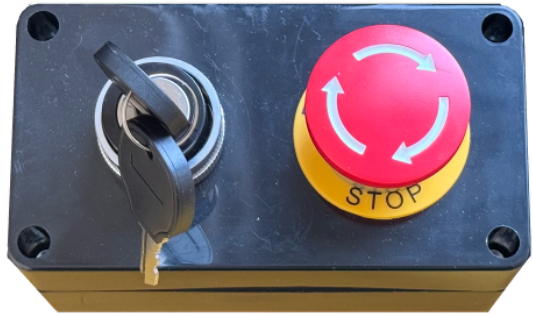
\includegraphics[width=0.7\textwidth]{assets/figures/Protections_laser/Securite_electrique/boitier_arret_urgence_maintenance.png}
    \end{center}
    \caption{Boîtier comprenant l'arrêt d'urgence et la clé de maintenance}
    \label{boitier_arret_urgence_maintenance}
\end{figure}

\section{Version finale du schéma électrique de l'interlock}
Une fois les capteurs choisis, le schéma électrique est remis à jour. Le changement a été fait au niveau des noms de bornes, afin qu'ils correspondent aux noms indiqués sur chaque capteur.

\begin{figure}[H]
    \begin{center}
        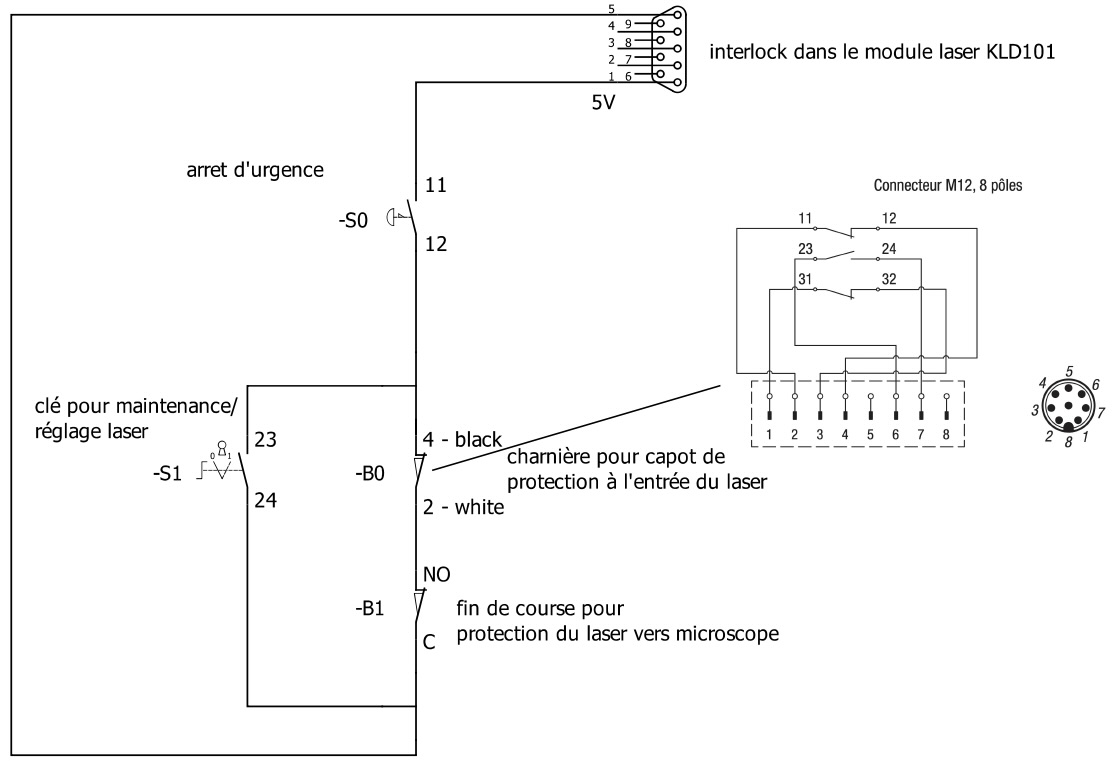
\includegraphics[width=\textwidth]{assets/figures/Protections_laser/Securite_electrique/interlock_schema_elec_V2.jpg}
    \end{center}
    \caption{Version finale du schéma électrique complet de l'interlock}
    \label{schema_interlock_v2}
\end{figure}

\section{Câblage de l'interlock}
\begin{minipage}[c]{0.48\textwidth}
    Une fois tous les composants en place, le câblage de l'interlock est exécuté. Sur la photo ci-contre, voir la Figure~\ref{cablage_vers_connecteur_laser}, le fil rouge et le fil noir sortent du connecteur du laser et seront utilisé pour le circuit de l'interlock.
\end{minipage}\hfill
\begin{minipage}[c]{0.48\textwidth}
    \begin{center}
        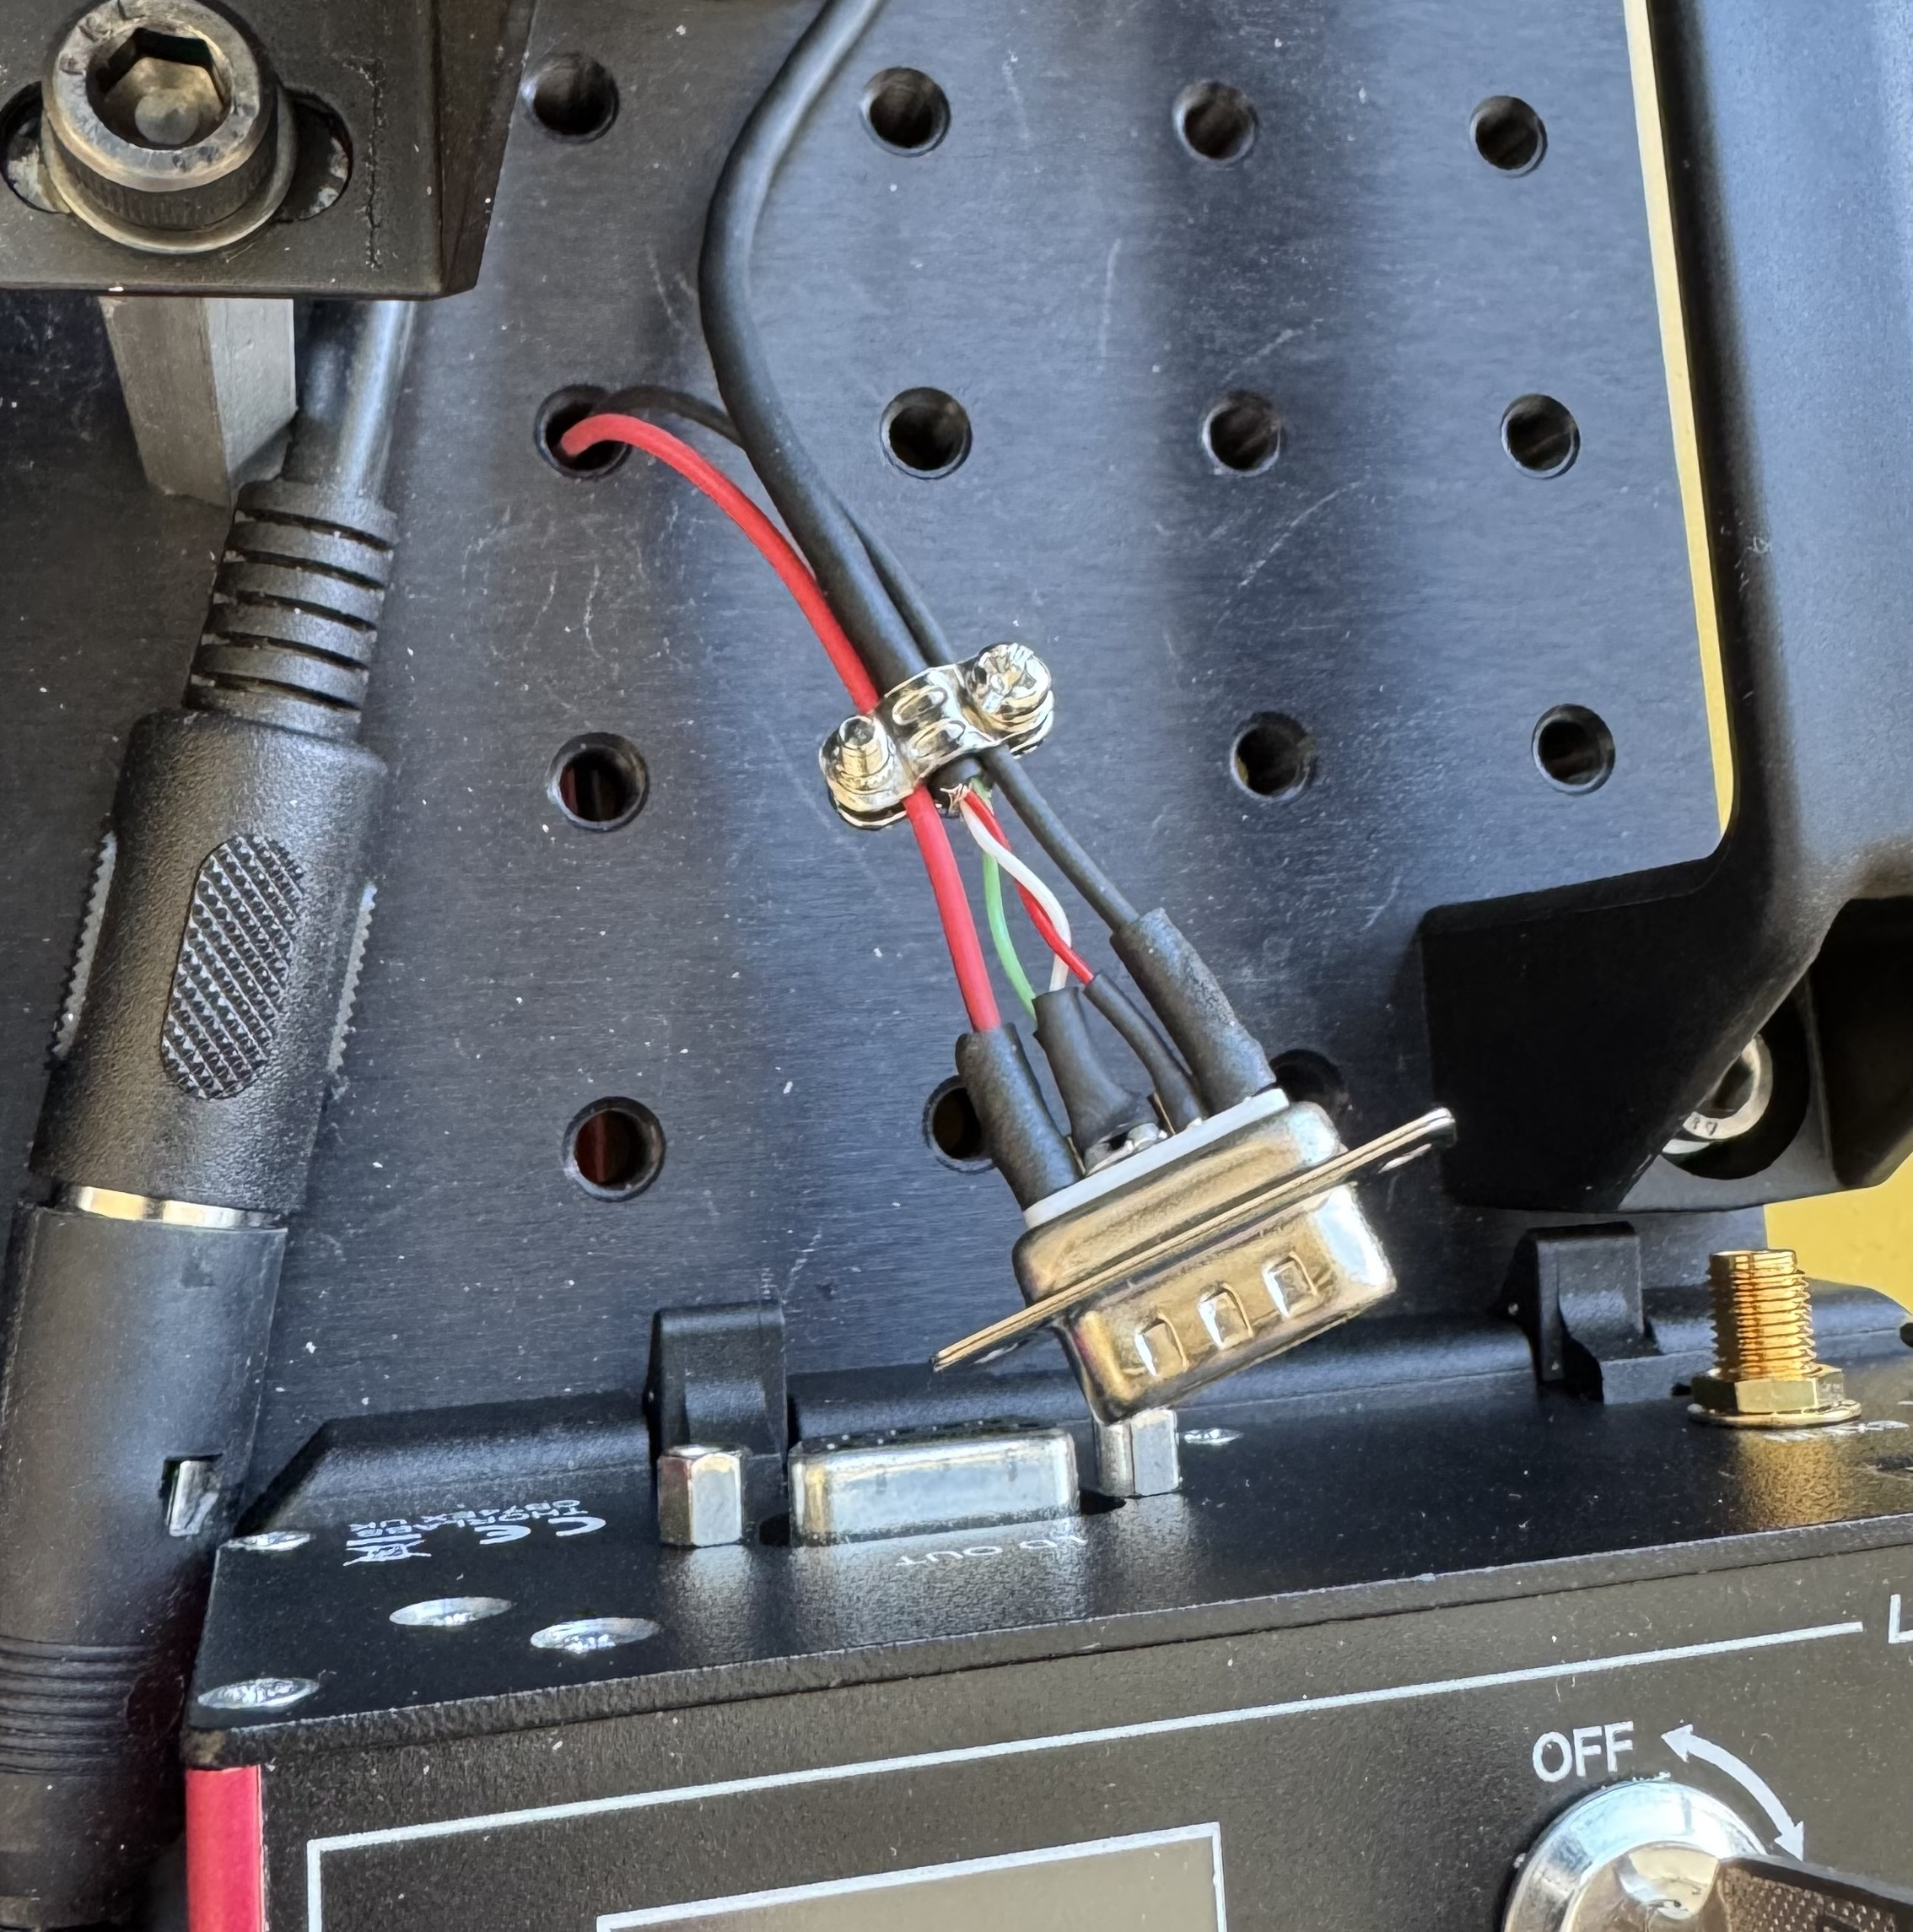
\includegraphics[width=0.9\textwidth]{assets/figures/Protections_laser/Securite_electrique/cablage_vers_connecteur_laser.jpeg}
    \end{center}
    \captionof{figure}{Connexion des deux fils, rouge et noir, sortant du connecteur du laser}
    \label{cablage_vers_connecteur_laser}
\end{minipage}

\begin{minipage}[c]{0.48\textwidth}
    Comme montré sur la Figure~\ref{cablage_sous_plaque_de_montage} ci-dessous, ces fils passent sous la plaque de montage en aluminium et rejoignent le boîtier contenant l'arrêt d'urgence et la clé de maintenance. Ceux-ci sont indiqués par la flèche \textcolor[RGB]{115, 210, 210}{bleue}.

    \vspace{1em}
    La flèche \textcolor{red}{rouge}, montre les deux fils reliant le contact normalement ouvert dans le fin de course. Eux aussi rejoignent le boîtier par dessous.
\end{minipage}\hfill
\begin{minipage}[c]{0.48\textwidth}
    \begin{center}
        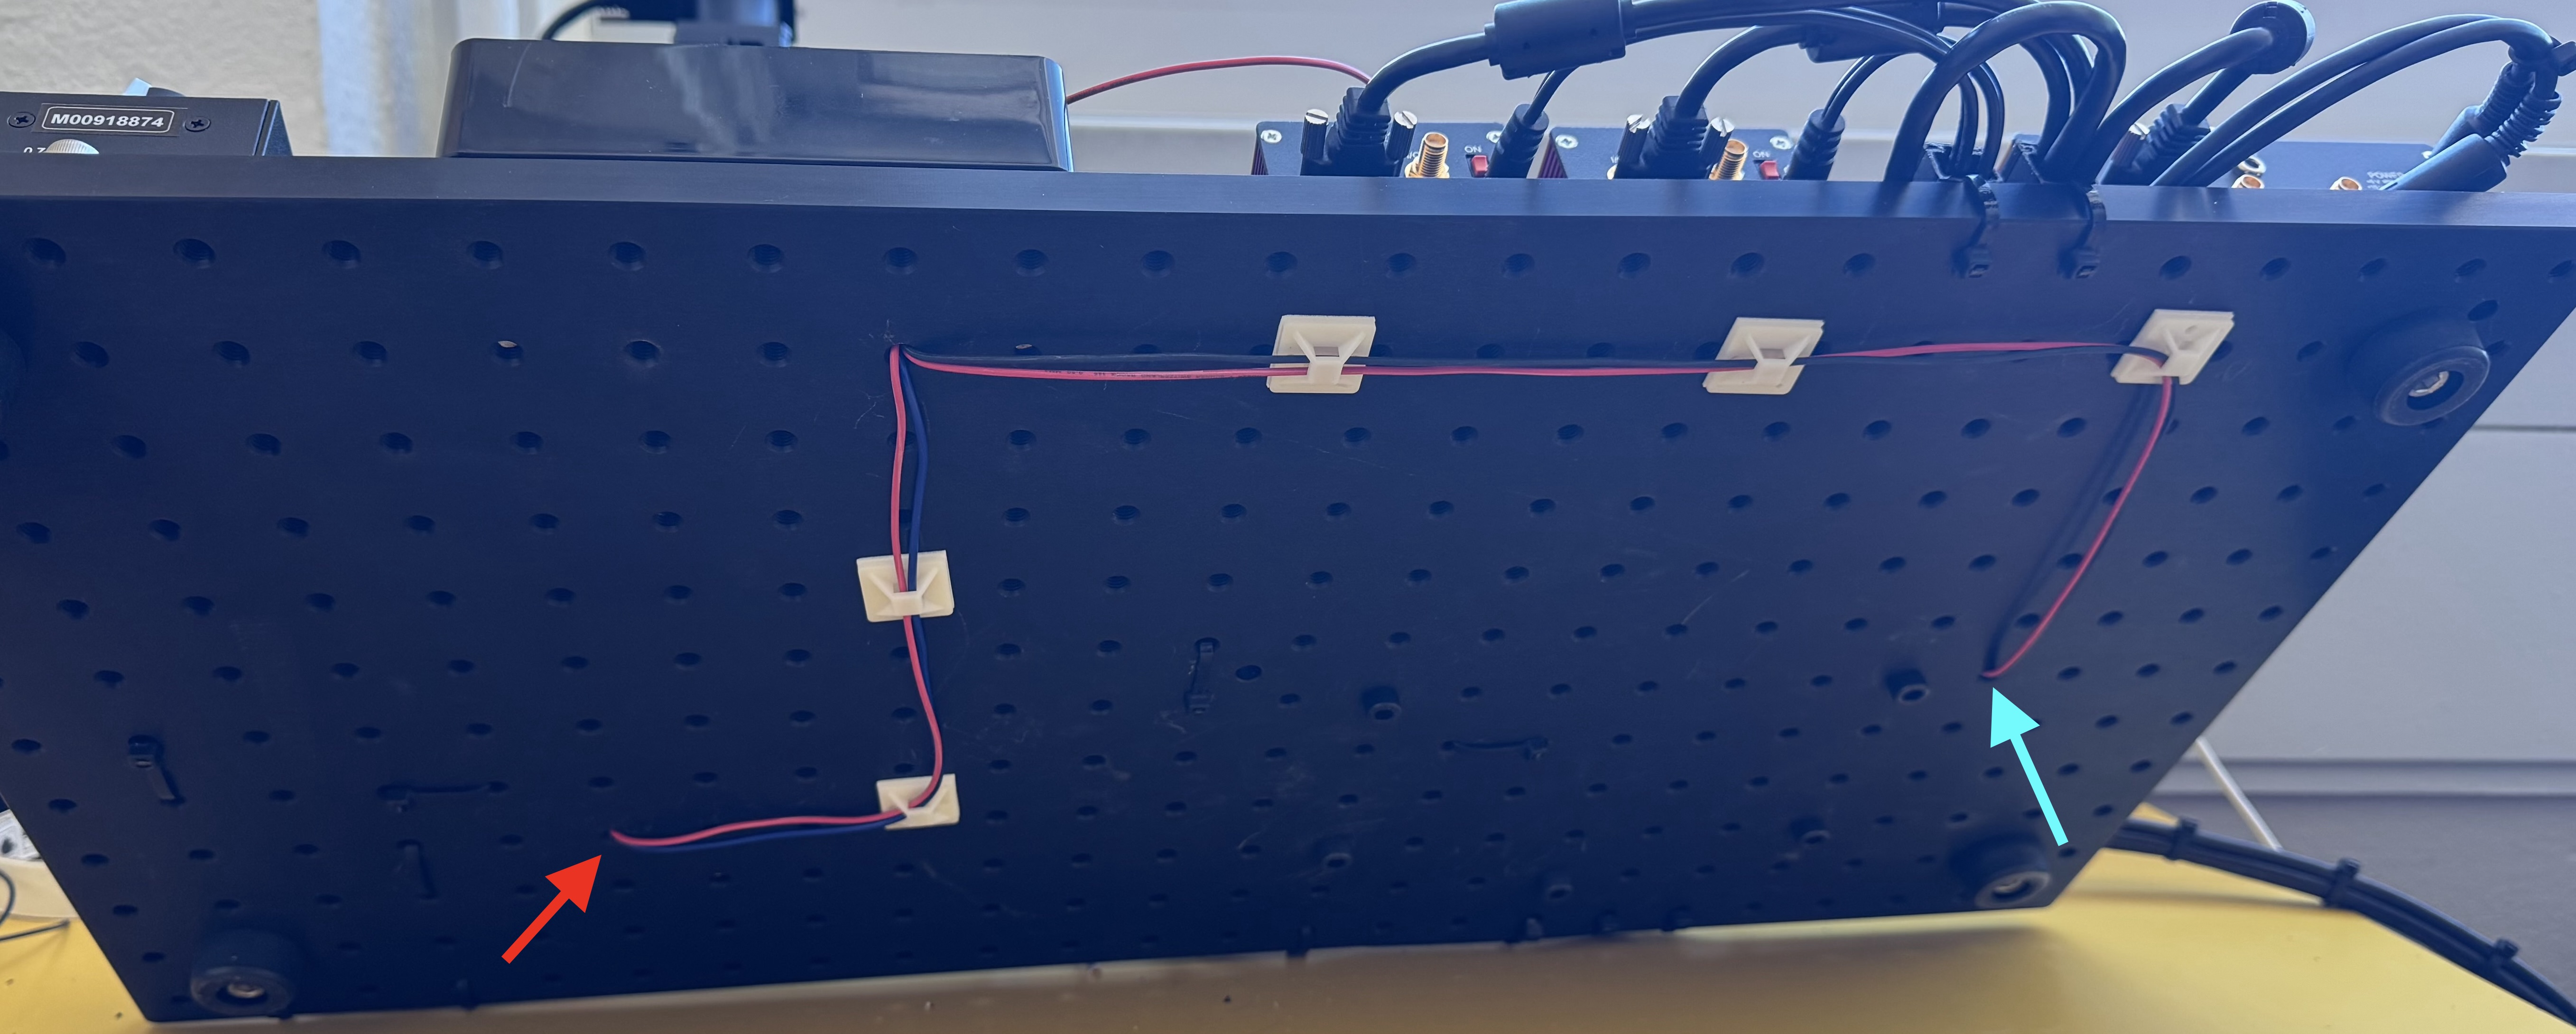
\includegraphics[width=\textwidth]{assets/figures/Protections_laser/Securite_electrique/cablage_sous_plaque_de_montage.jpeg}
    \end{center}
    \captionof{figure}{Passage des deux fils de l'interlock sous la plaque de montage en aluminium}
    \label{cablage_sous_plaque_de_montage}
\end{minipage}

\begin{minipage}[c]{0.48\textwidth}
    Finalement, en suivant le schéma électrique (Figure~\ref{schema_interlock_v2}), tous les composants de sécurité se retrouvent dans le boîtier, afin d'être connecté ensemble, comme illustré sur la Figure~\ref{cablage_dans_boitier}, ci-contre.
\end{minipage}\hfill
\begin{minipage}[c]{0.48\textwidth}
    \begin{center}
        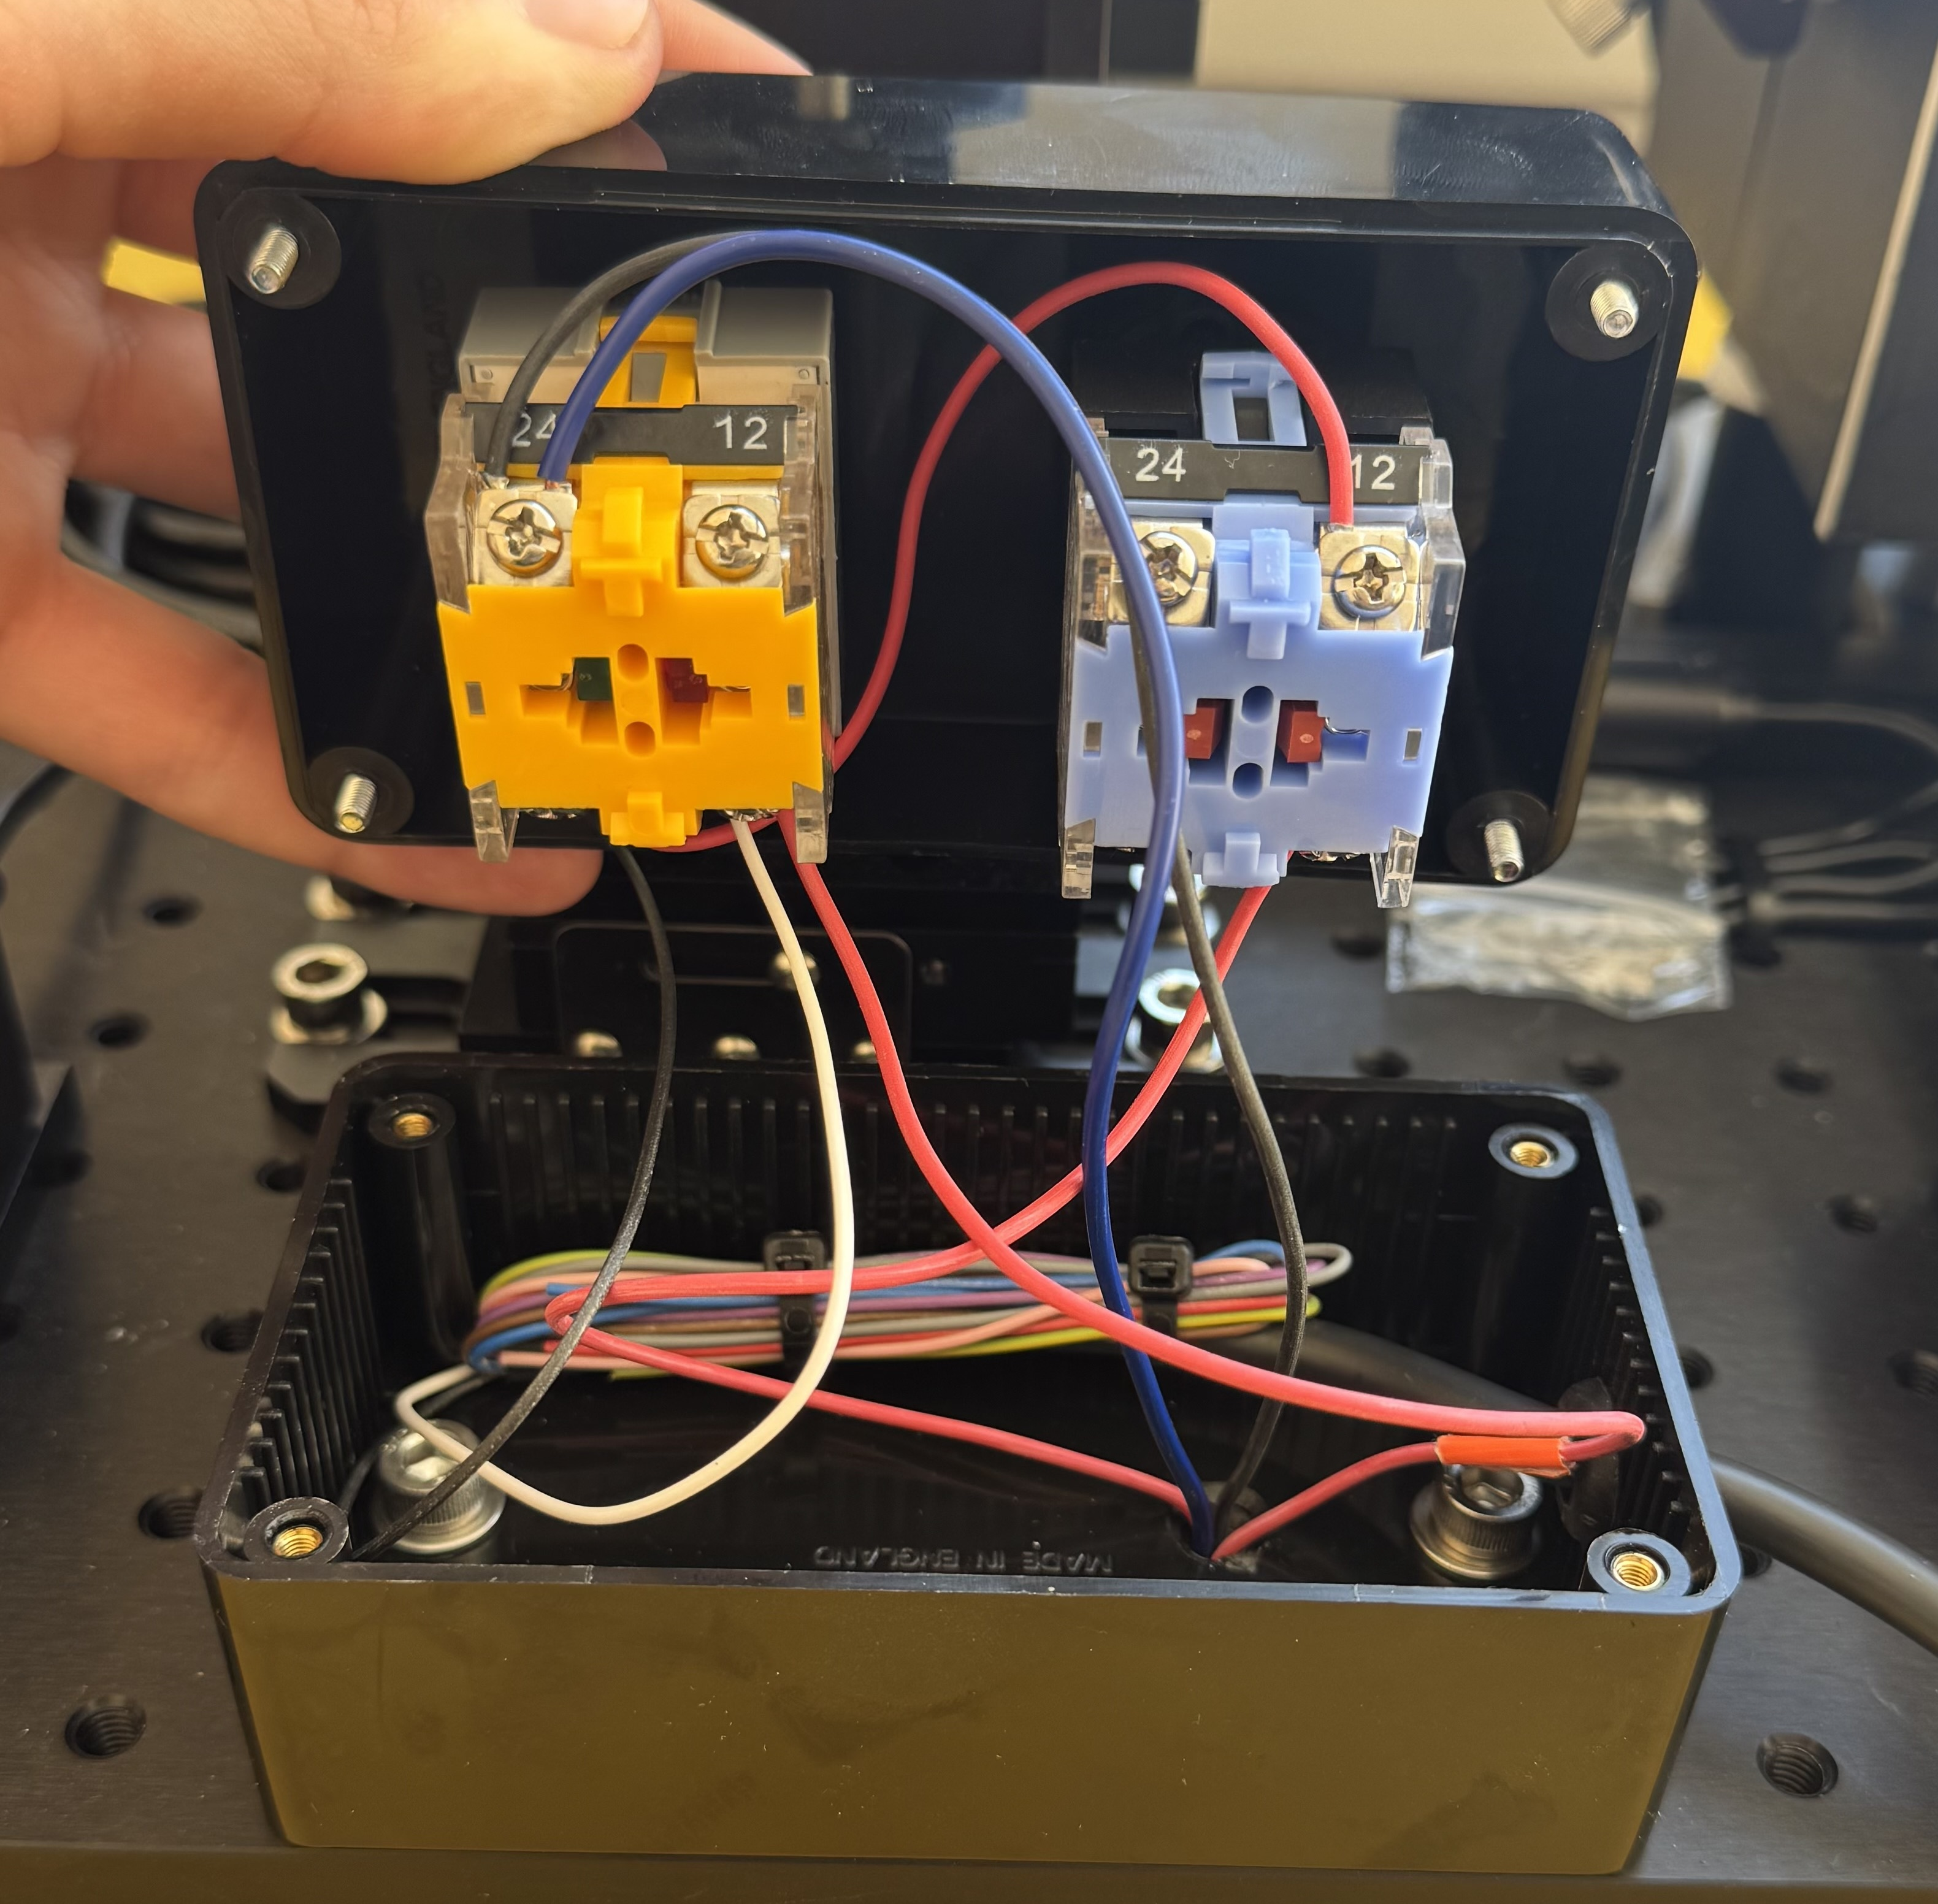
\includegraphics[width=\textwidth]{assets/figures/Protections_laser/Securite_electrique/cablage_dans_boitier.jpeg}
    \end{center}
    \captionof{figure}{Câblage des composants de sécurité dans le boîtier}
    \label{cablage_dans_boitier}
\end{minipage}
\chapter{Sécurité mécanique} \label{chapter:securite_mecanique}
\section{Exigences fonctionnelles des protections}
Cette section a pour but de détailler les différentes exigences que les deux protections vont devoir remplir.

Les protections :
\begin{enumerate}
    \item assureront une protection complète contre les réflexions du laser, afin de garantir la sécurité des utilisateurs du kit.
    \item ne devront pas restreindre l'accessibilité des autres composants, tels que les lentilles réglables ainsi que le laser, afin de pouvoir régler ceux-ci facilement, si nécessaire.
    \item seront des assemblages mécaniques simples à monter et à démonter.
    \item auront une conception simple, afin que leur fabrication soit la plus aisée possible.
    \item comprendront le moins de pièces et de visseries possible.
\end{enumerate}

\section{Protection à l'entrée du laser}
Cette section va expliquer les différentes étapes de la conception de la protection à l'entrée du laser, la modélisation de celle-ci, les prototypes qui ont été réalisés, la fabrication final ainsi que le montage.
\subsection{Prototype initial en carton}
Lorsqu'il est possible de faire un prototype en carton, je le fais afin d'avoir une première idée concrète du projet à réaliser. Ses avantages résident dans le fait que c'est rapide à créer et simple. La première idée a direct été une boîte qui entoure la cage de lentille avec un système de capot qui peut se soulever. Ci-dessous, deux photos du prototype en carton, avec une photo où le capot est fermée, voir Figure \ref{carton_protection_fermee}, et l'autre photo quand la protection est ouverte, voir Figure \ref{carton_protection_ouverte}.

\begin{minipage}[c]{0.48\textwidth}
    \begin{center}
        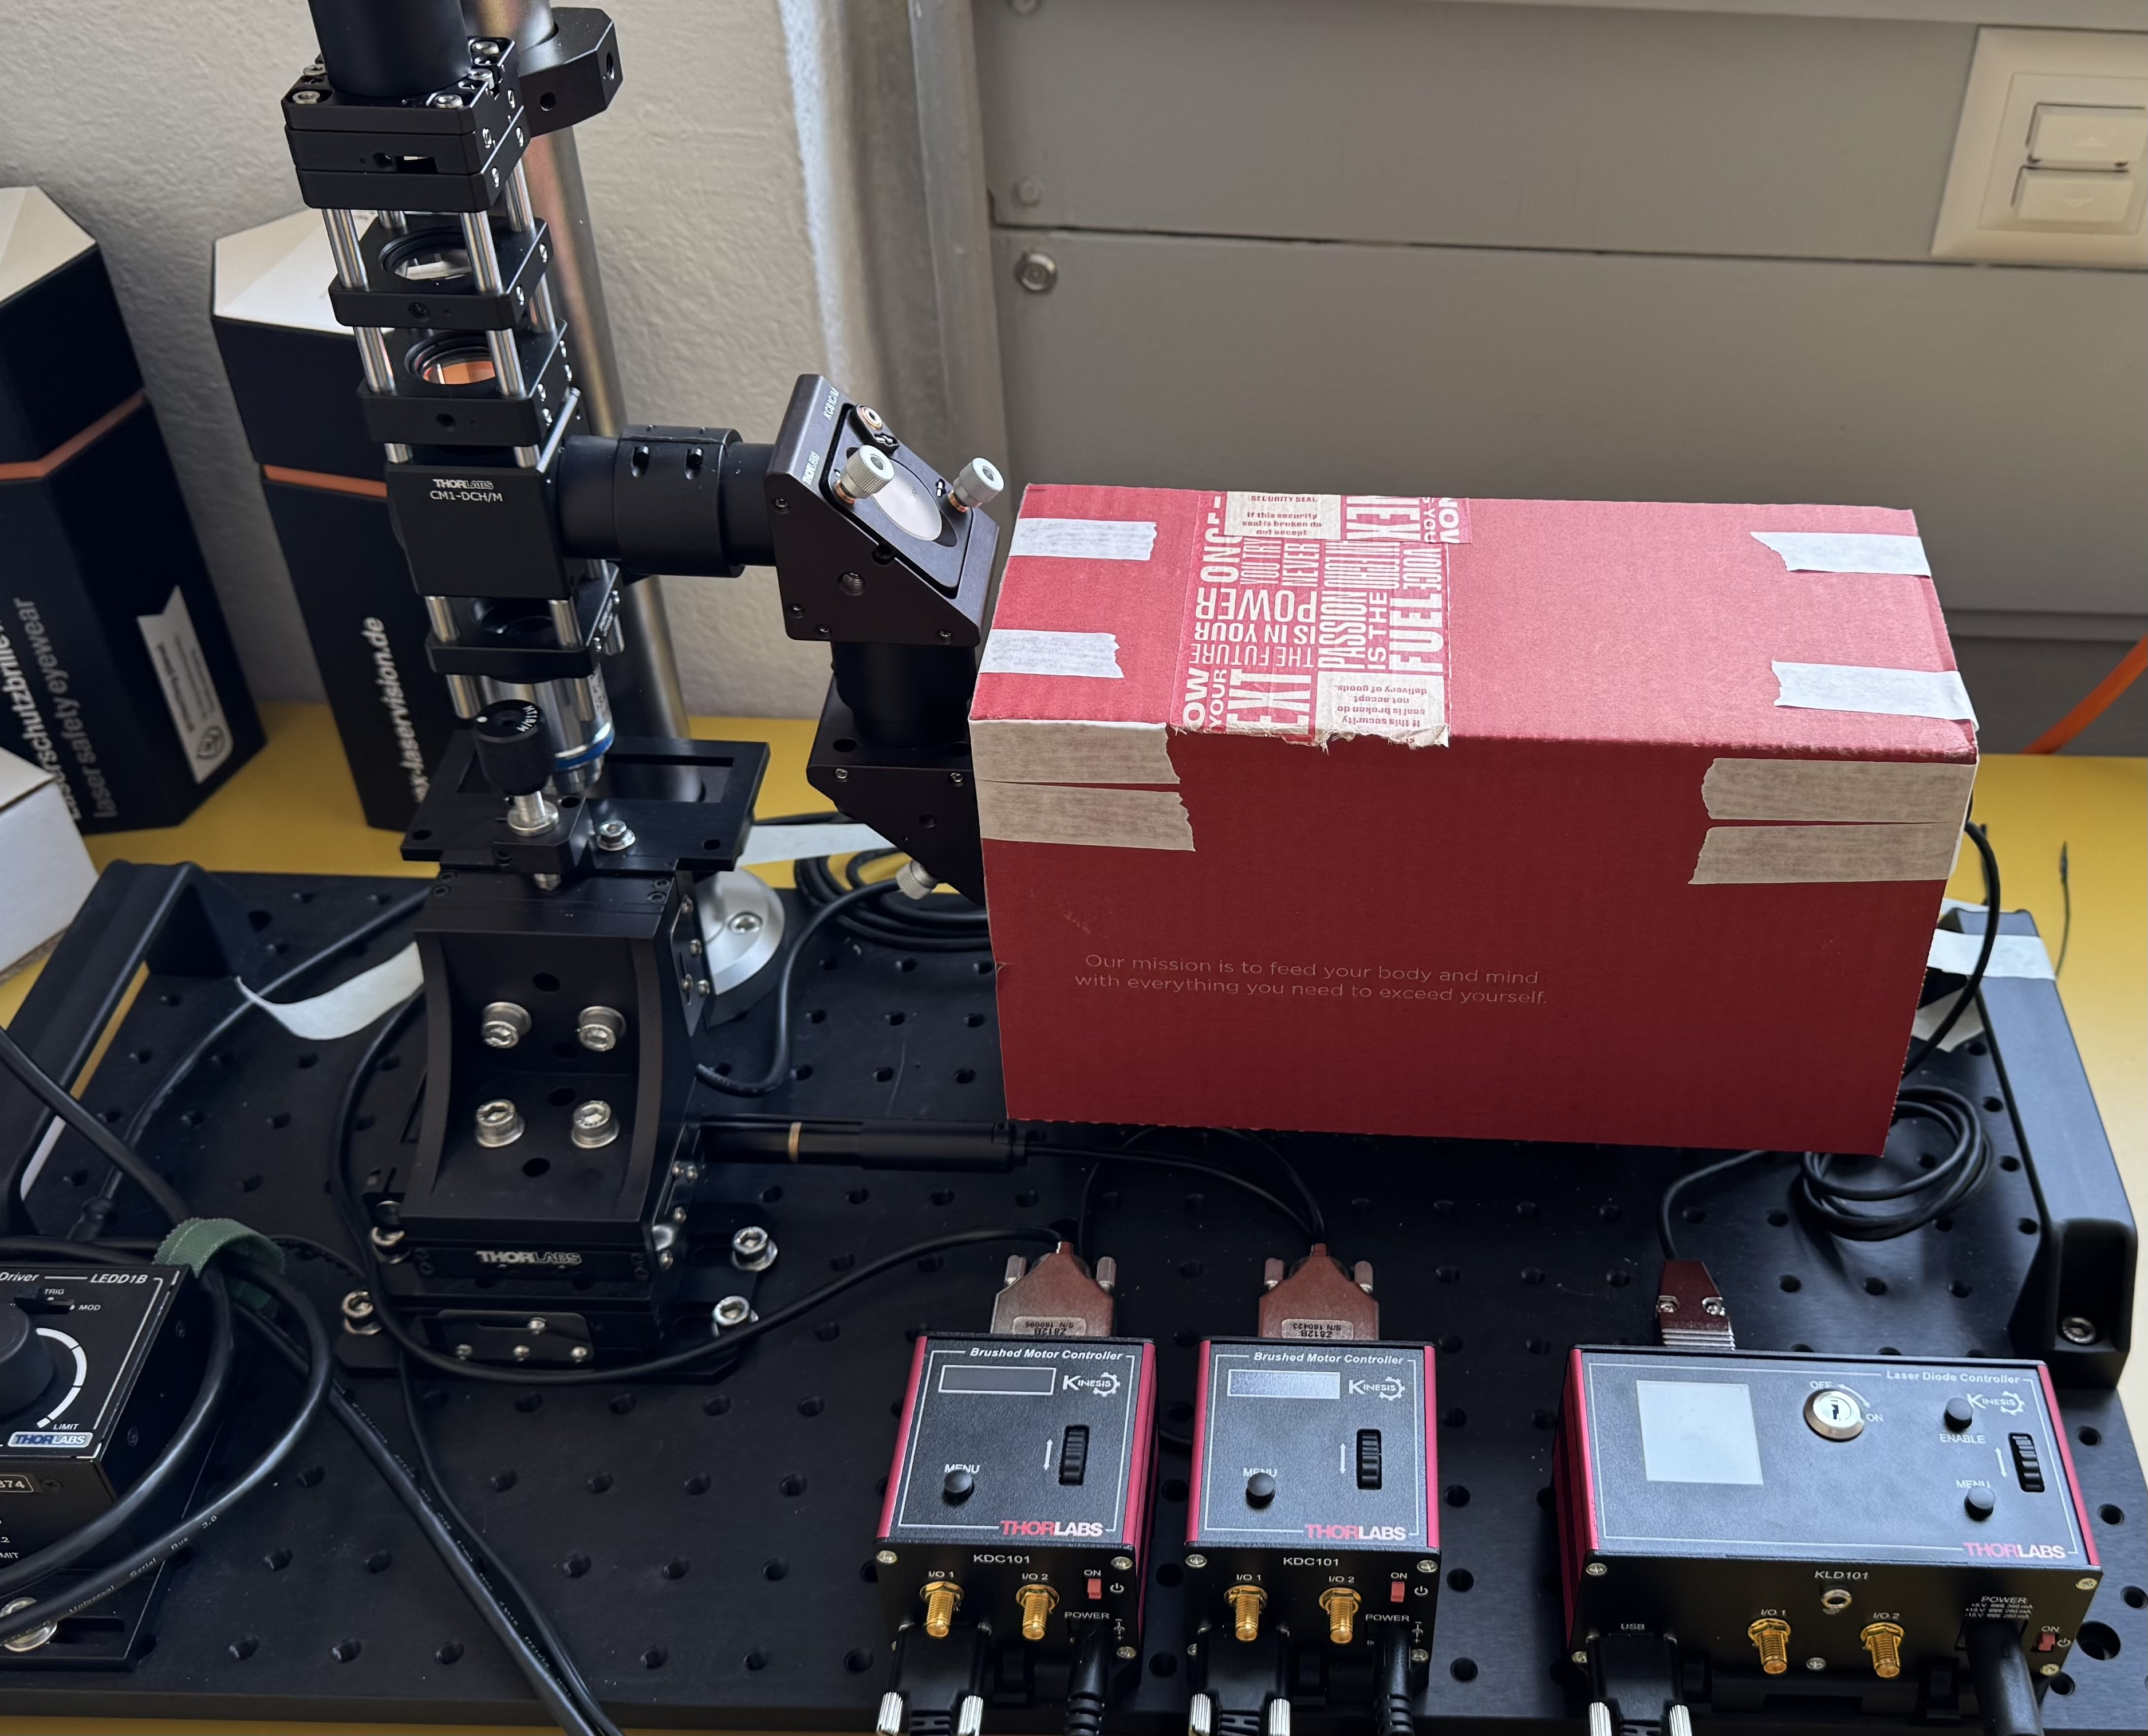
\includegraphics[width=\textwidth]{assets/figures/Protections_laser/Securite_mecanique/Protection_entree_laser/carton_protection_ferme.jpeg}
    \end{center}
    \captionof{figure}{Prototype en carton, protection fermée}
    \label{carton_protection_fermee}
\end{minipage}\hfill
\begin{minipage}[c]{0.48\textwidth}
    \begin{center}
        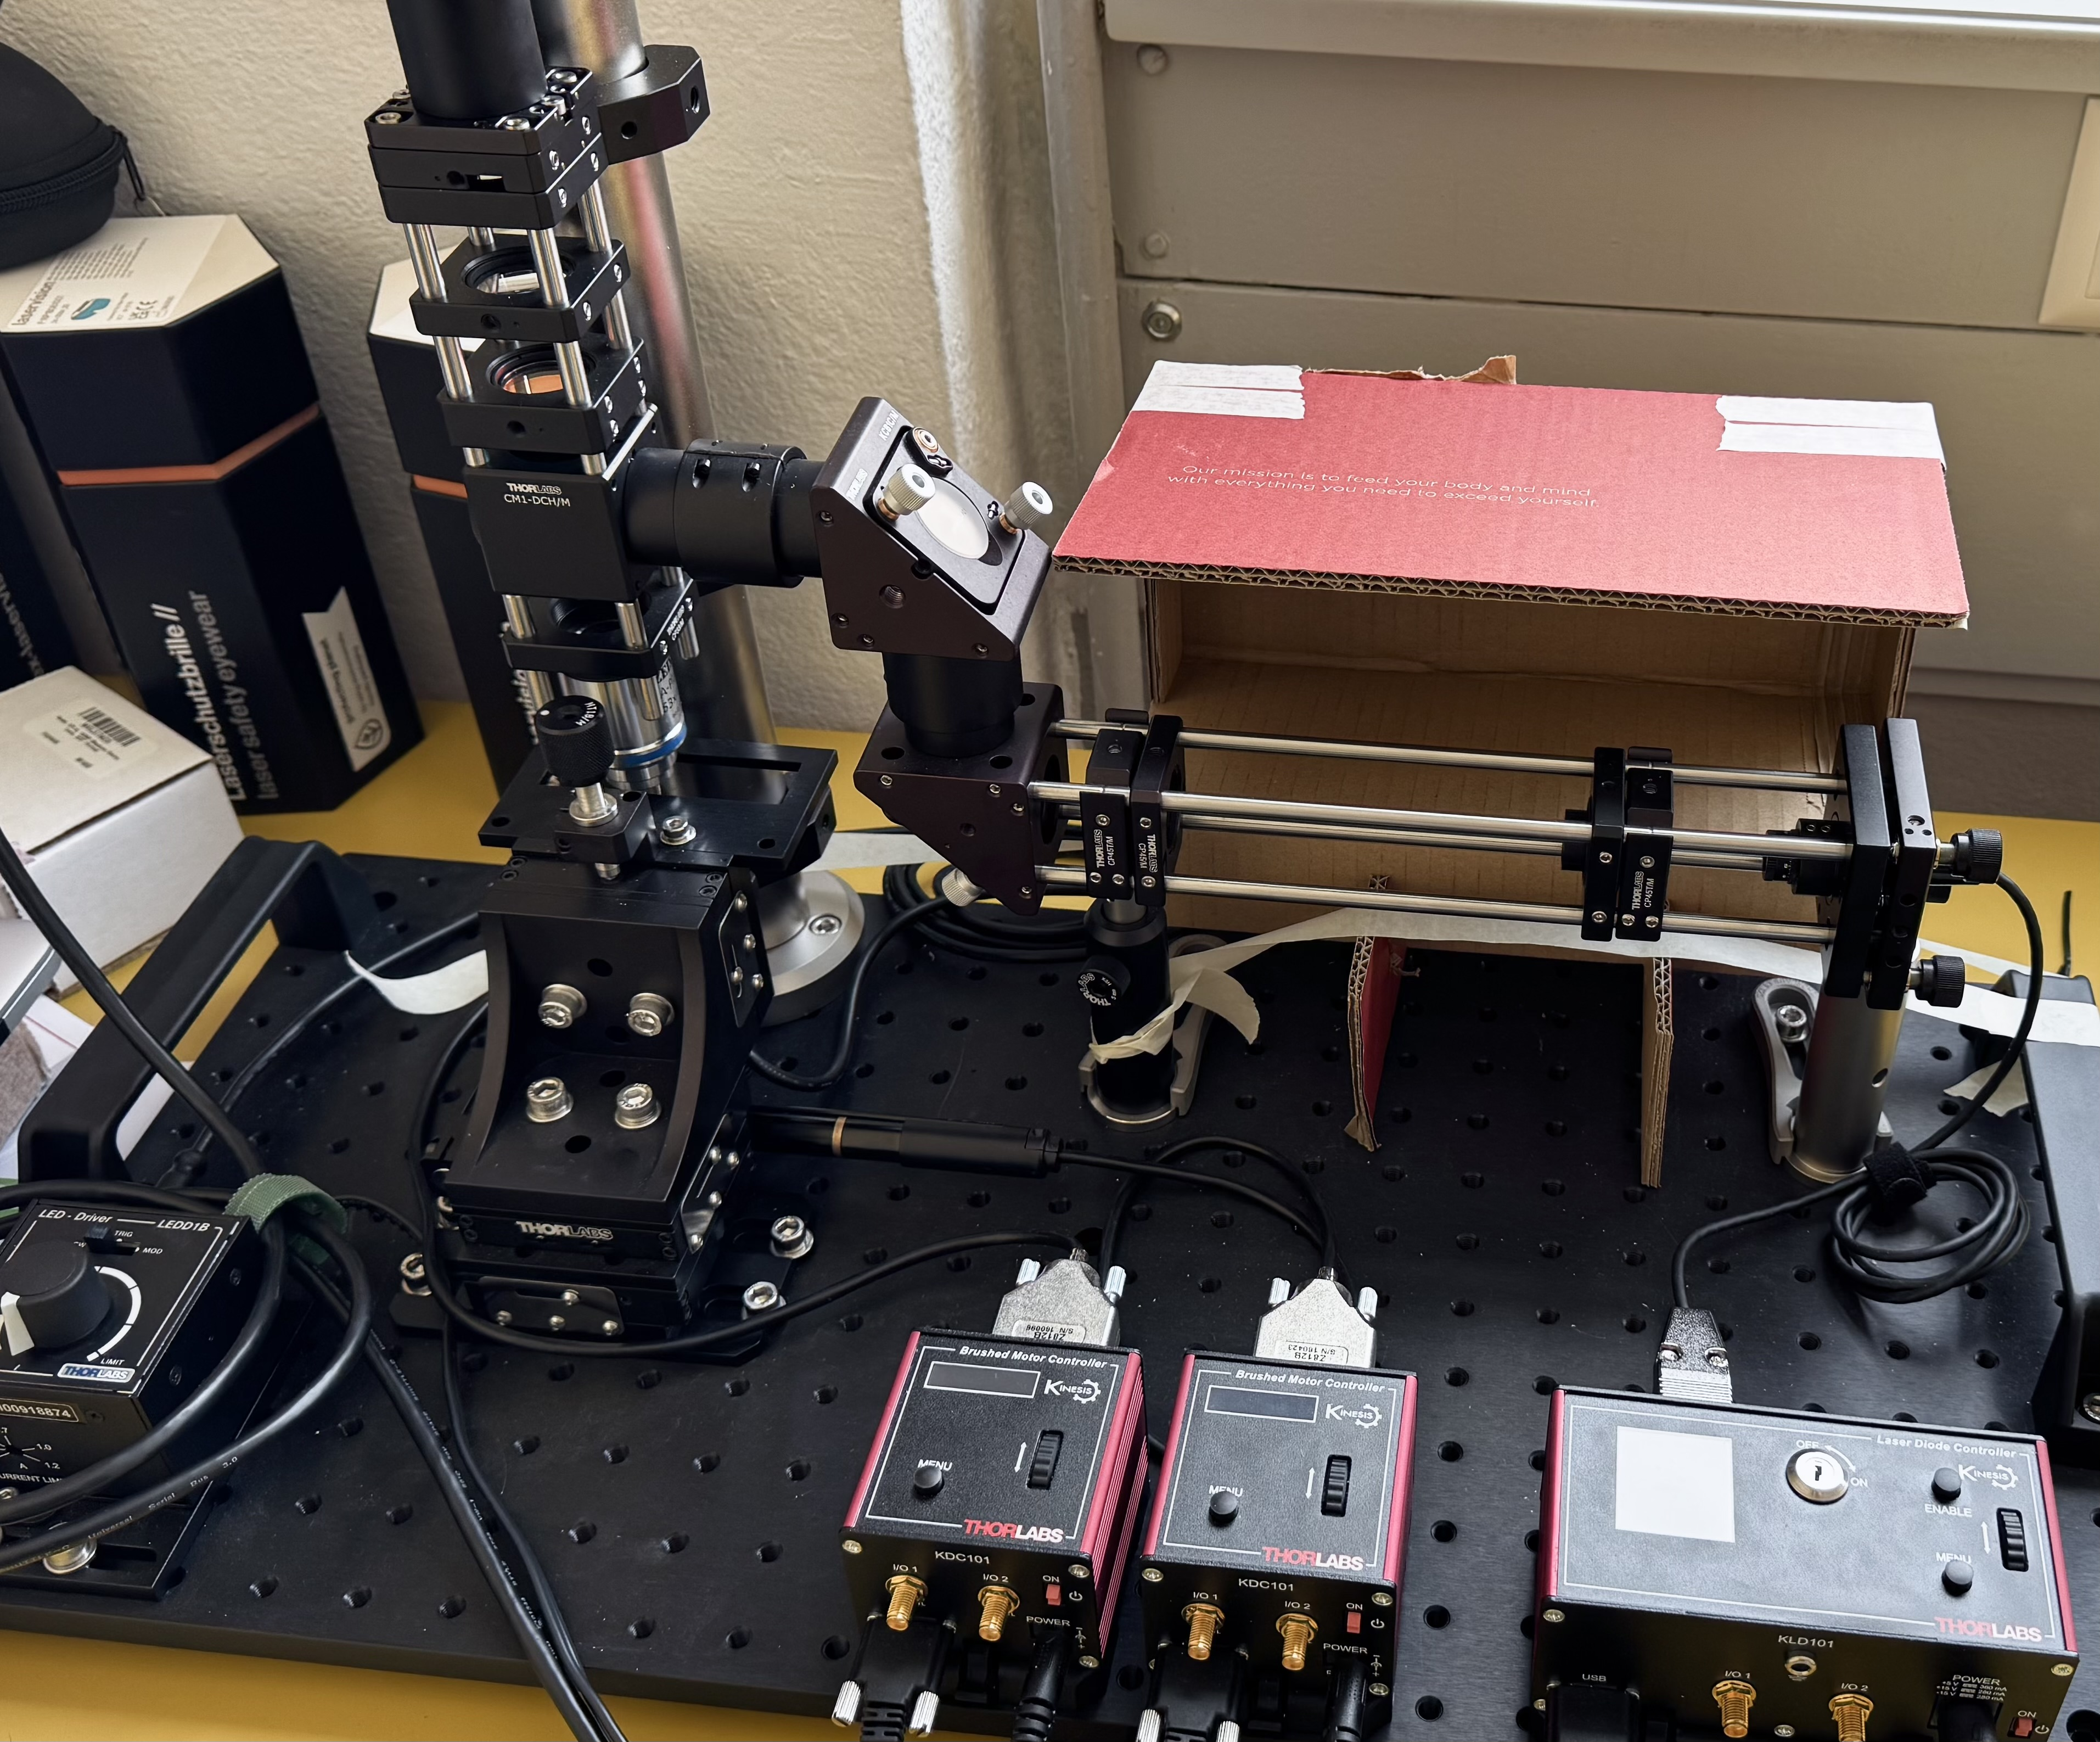
\includegraphics[width=\textwidth]{assets/figures/Protections_laser/Securite_mecanique/Protection_entree_laser/carton_protection_ouvert.jpeg}
    \end{center}
    \captionof{figure}{Prototype en carton, protection ouverte}
    \label{carton_protection_ouverte}
\end{minipage}

\subsection{Modélisation de la protection}
Maintenant que l'idée principale est là, il faut passer à la modélisation de la protection. Avant cette étape, la représentation en 3D du kit complet a été faite, comme expliqué à la page~\pageref{modelisation_3D} au premier paragraphe. Le 3D du kit permet de pouvoir créer la protection en tenant compte de  toutes les contraintes liés aux autres composants, sans devoir faire des mesures sur le kit réel.

Pour pouvoir mieux comprendre les choix de conception et les étapes faites pour réaliser la protection, les Figures~\ref{model_3D_ferme}~et~\ref{model_3D_ouvert}, ci-dessous, représente la modélisation complète de la protection ouverte et fermée.

\begin{minipage}[c]{0.48\textwidth}
    \begin{center}
        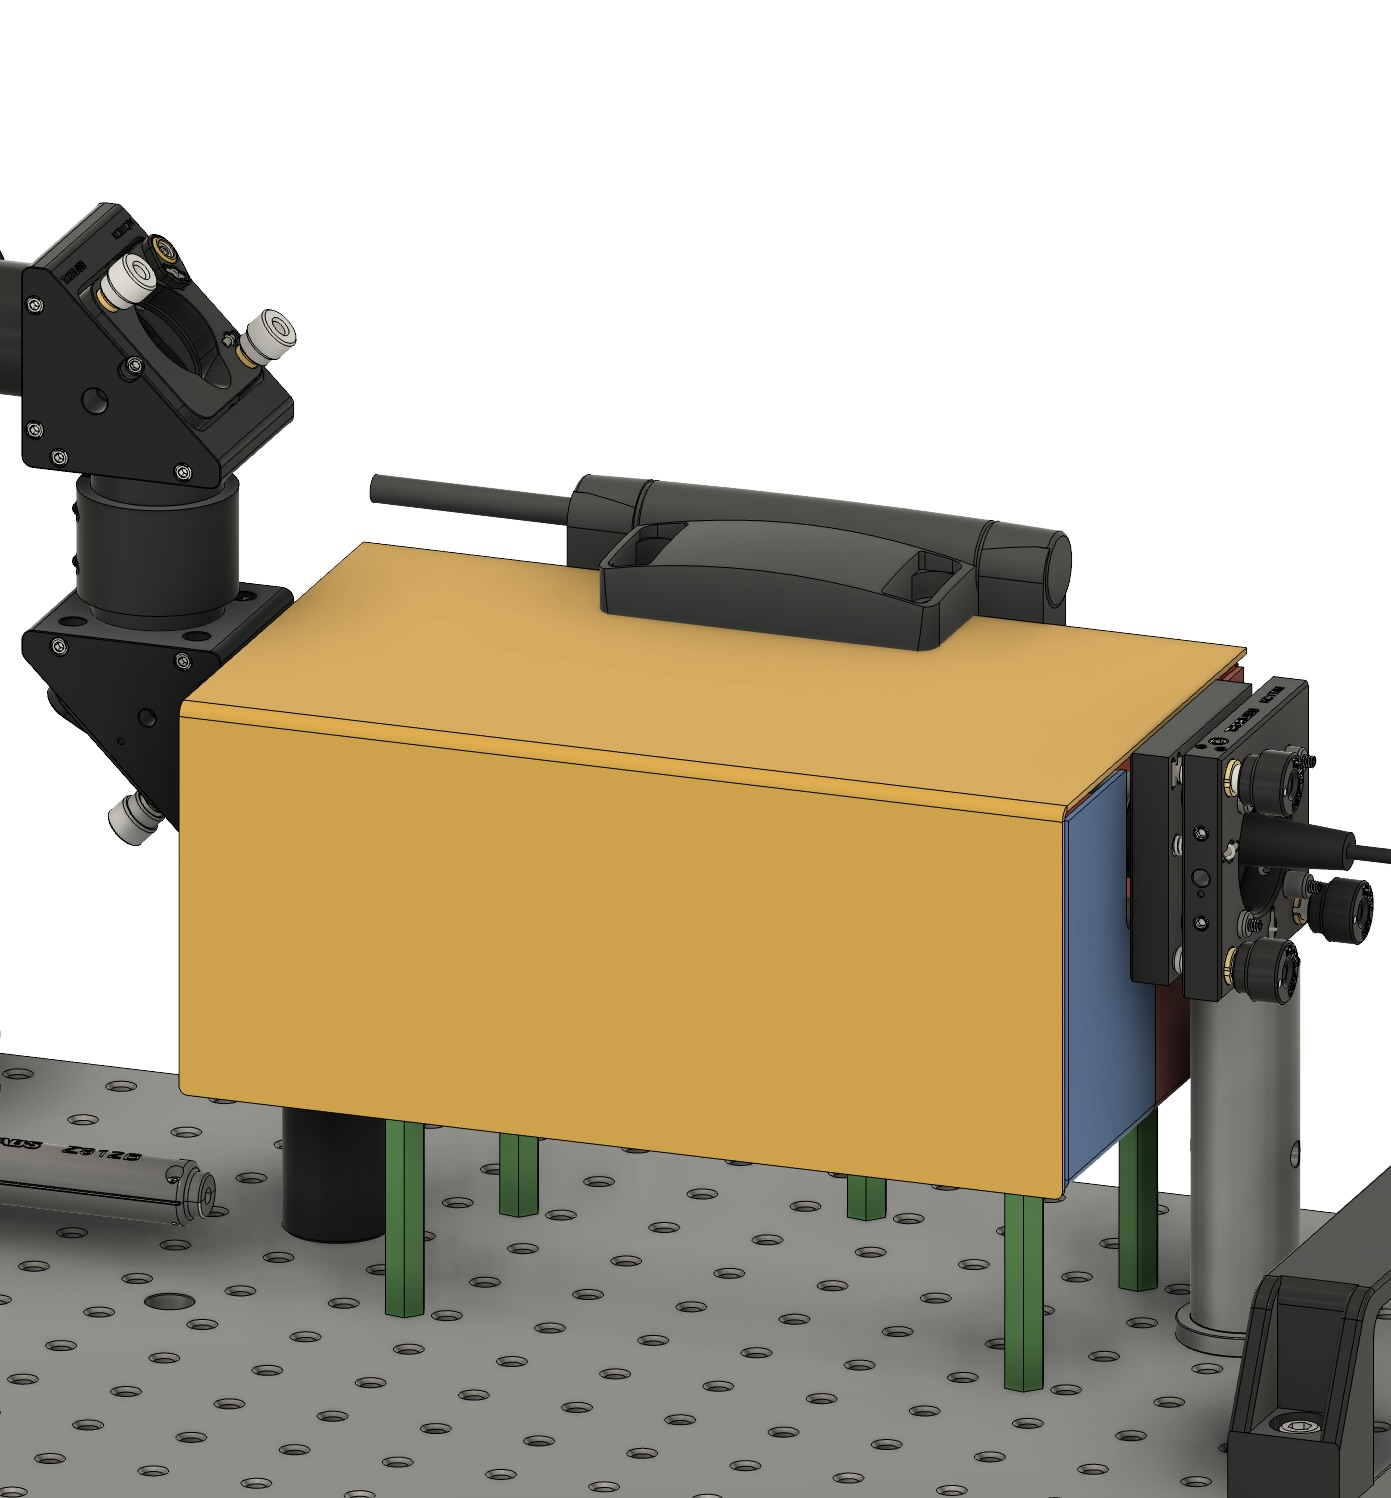
\includegraphics[width=\textwidth]{assets/figures/Protections_laser/Securite_mecanique/Protection_entree_laser/model_3D_ferme.jpeg}
    \end{center}
    \captionof{figure}{Modèle 3D de la protection ouverte}
    \label{model_3D_ferme}
\end{minipage}\hfill
\begin{minipage}[c]{0.48\textwidth}
    \begin{center}
        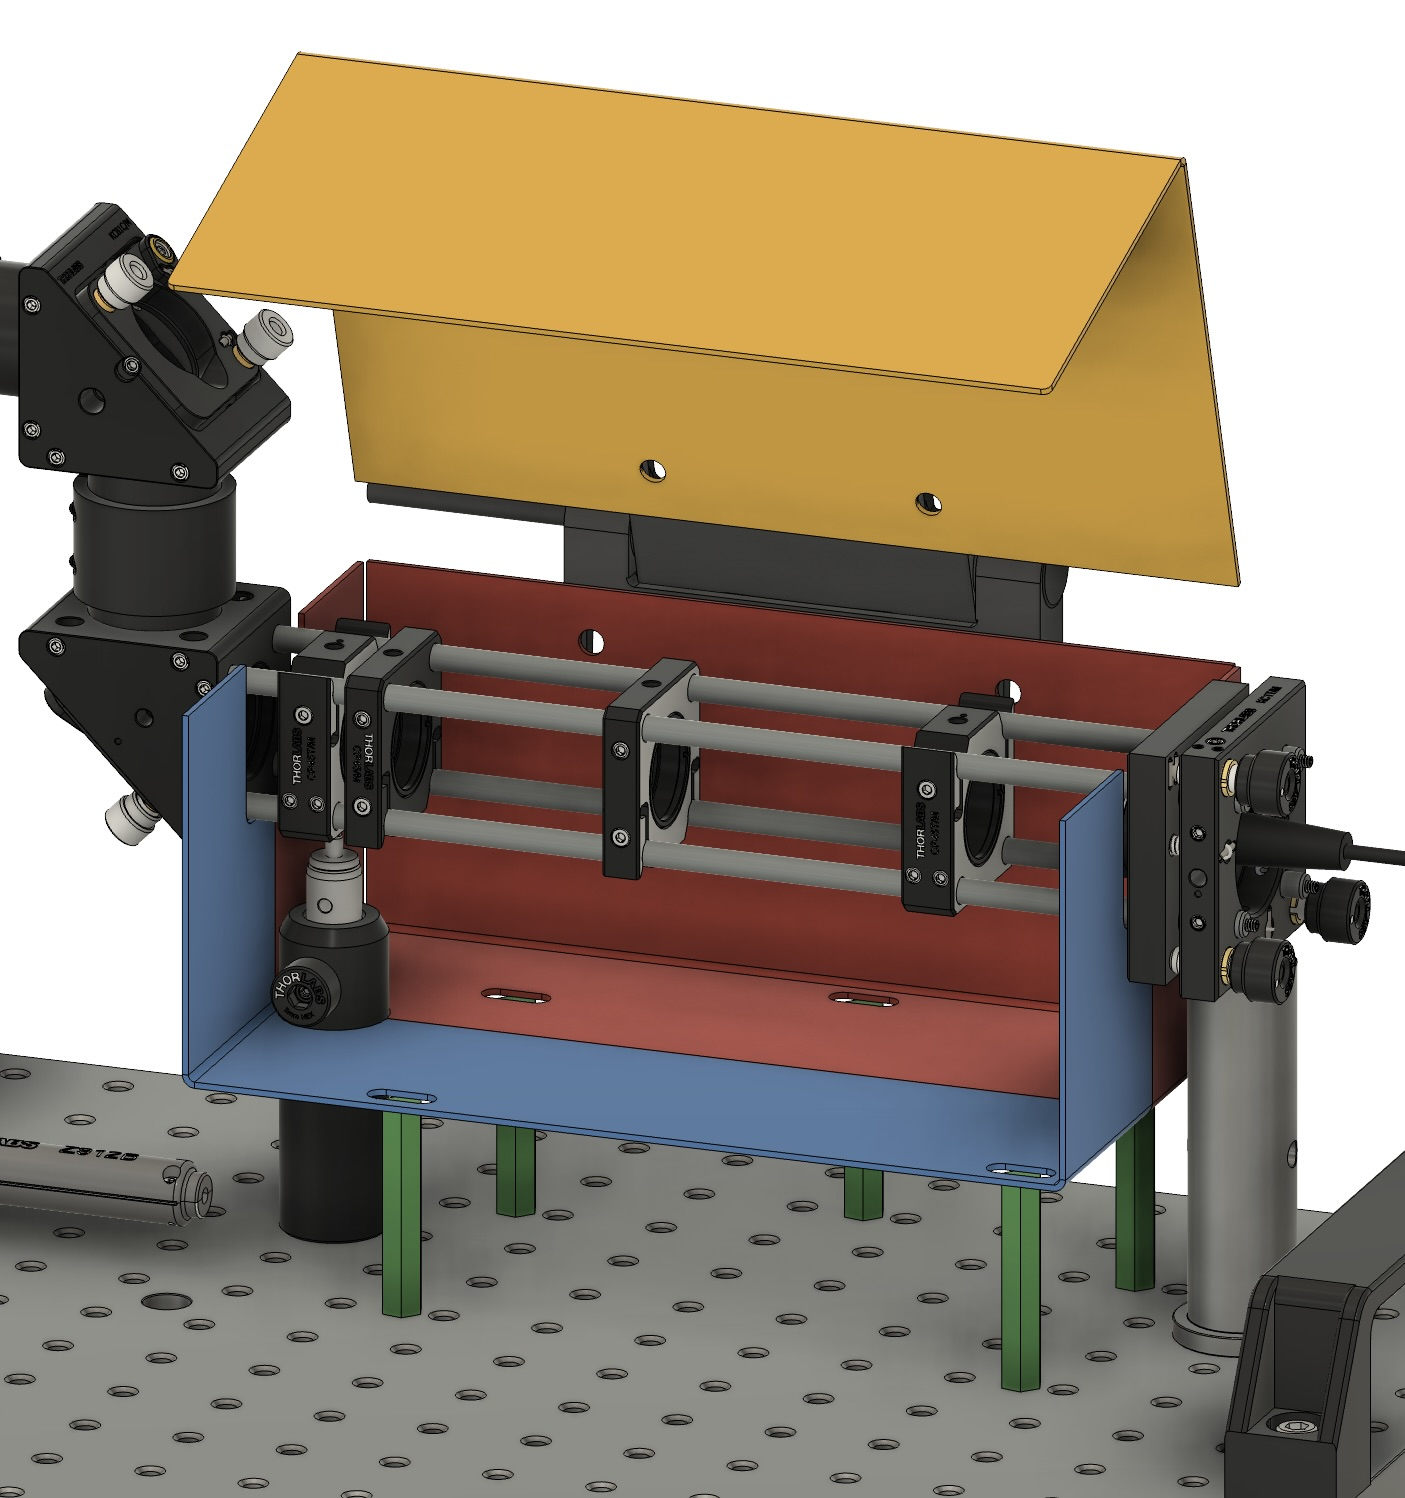
\includegraphics[width=\textwidth]{assets/figures/Protections_laser/Securite_mecanique/Protection_entree_laser/model_3D_ouvert.jpeg}
    \end{center}
    \captionof{figure}{Modèle 3D de la protection fermée}
    \label{model_3D_ouvert}
\end{minipage}

\begin{table}[H]
    \centering
    \caption{Nomenclature des pièces modélisées avec code couleur pour la protection à l'entrée du laser}
    \begin{tabular}{|c|l|}
        \hline
        \textbf{Couleur}                           & \textbf{Nom de la pièce}                    \\
        \hline
        \textcolor[RGB]{88, 122, 163}{Bleu}        & Capot inférieur avant                       \\
        \textcolor[RGB]{170, 80, 70}{Rouge}        & Capot inférieur arrière                     \\
        \textcolor[RGB]{233, 173, 56}{Jaune}       & Capot supérieur                             \\
        \textcolor[RGB]{100, 100, 100}{Gris foncé} & Charnière reliant les capots inférieurs     \\
        \textcolor[RGB]{70, 170, 70}{Vert}         & Entretoises suportant les capots inférieurs \\
        \hline
    \end{tabular}
    \label{tab:nomenclature_pieces_laser}
\end{table}

\subsubsection{Contraintes rencontrées}

\begin{minipage}[c]{0.4\textwidth}
    La première contrainte a été cet axe noir vertical que l'on voit par la flèche noir sur la Figure~\ref{contrainte_axe_vertical} qui passent à travers les deux capots inférieurs.

    La solution s'est résumé à séparer le capot inférieur en deux, pour pouvoir assembler facilement sans devoir démonter des pièces du kit original.
\end{minipage}\hfill
\begin{minipage}[c]{0.58\textwidth}
    \begin{center}
        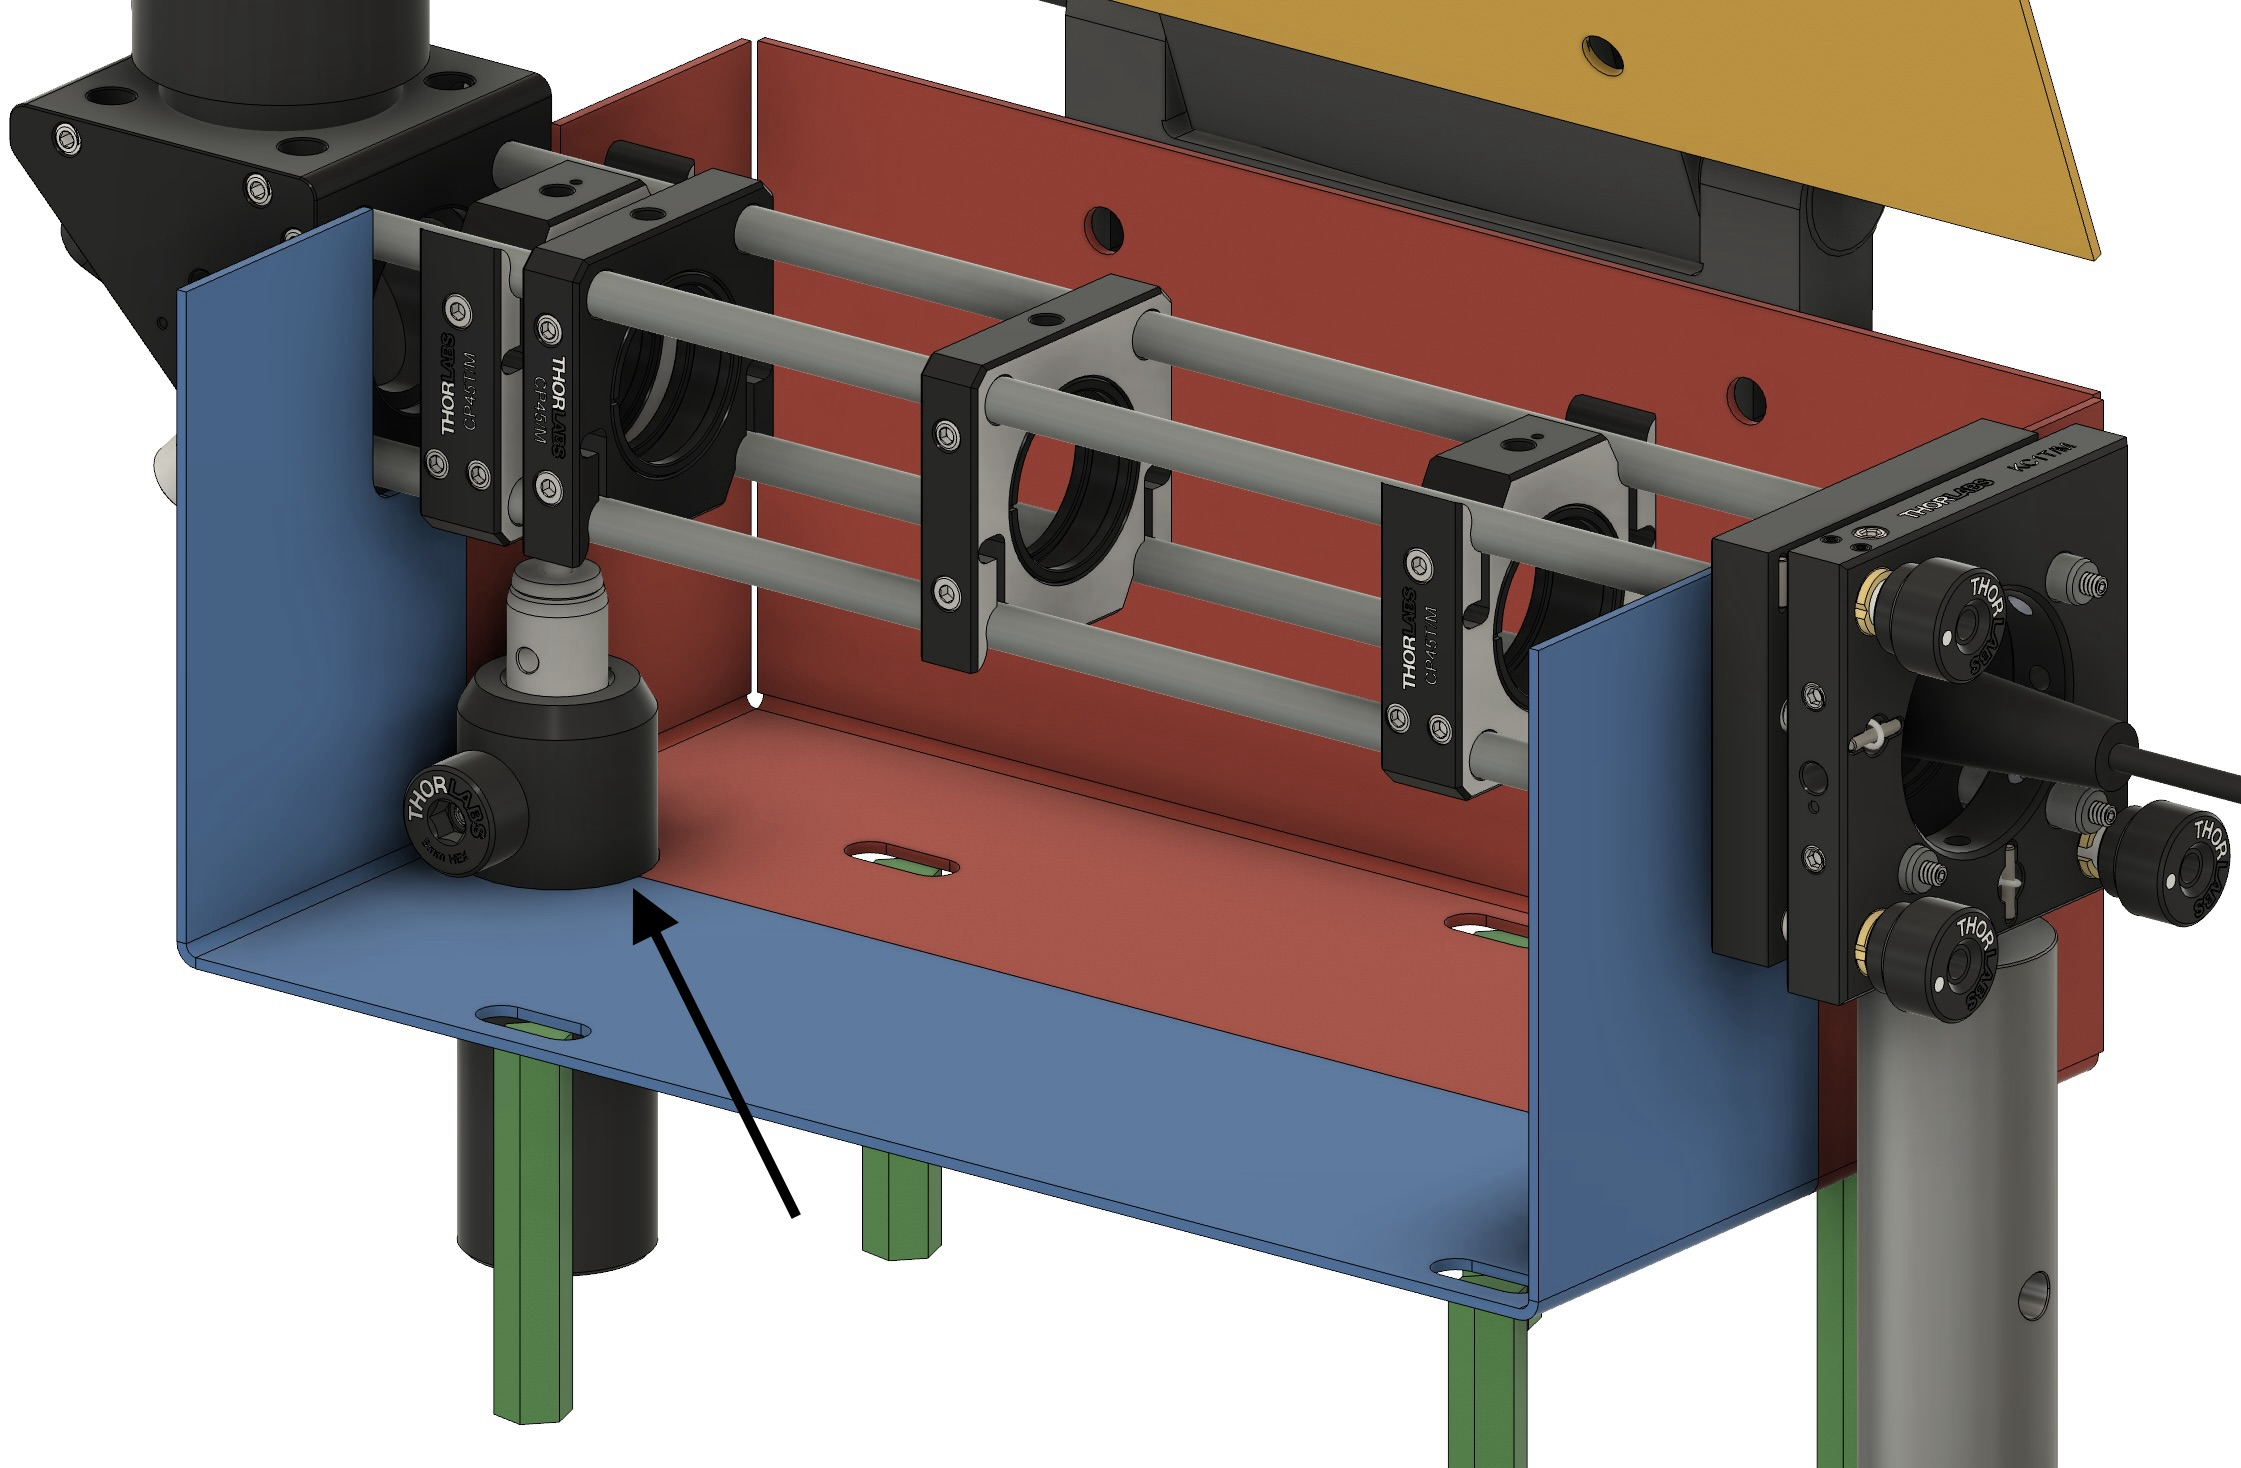
\includegraphics[width=\textwidth]{assets/figures/Protections_laser/Securite_mecanique/Protection_entree_laser/contrainte_axe_vertical.jpeg}
    \end{center}
    \captionof{figure}{Vue en perspective cavalière: Axe vertical traversant les protections inférieures}
    \label{contrainte_axe_vertical}
\end{minipage}

\begin{minipage}[c]{0.4\textwidth}
    Une contrainte supplémentaire a été cette vis de réglage indiquée par la flèche noir sur la Figure~\ref{contrainte_vis}. Elle se situe dans la course du capot supérieur.

    La solution retenue a été de s'assurer que toutes les protections, dans le plan horizontal, ne dépassent pas la largeur de la vis. Cette contrainte en entraîne une autre, qui sera détaillée ensuite.
\end{minipage}\hfill
\begin{minipage}[c]{0.58\textwidth}
    \begin{center}
        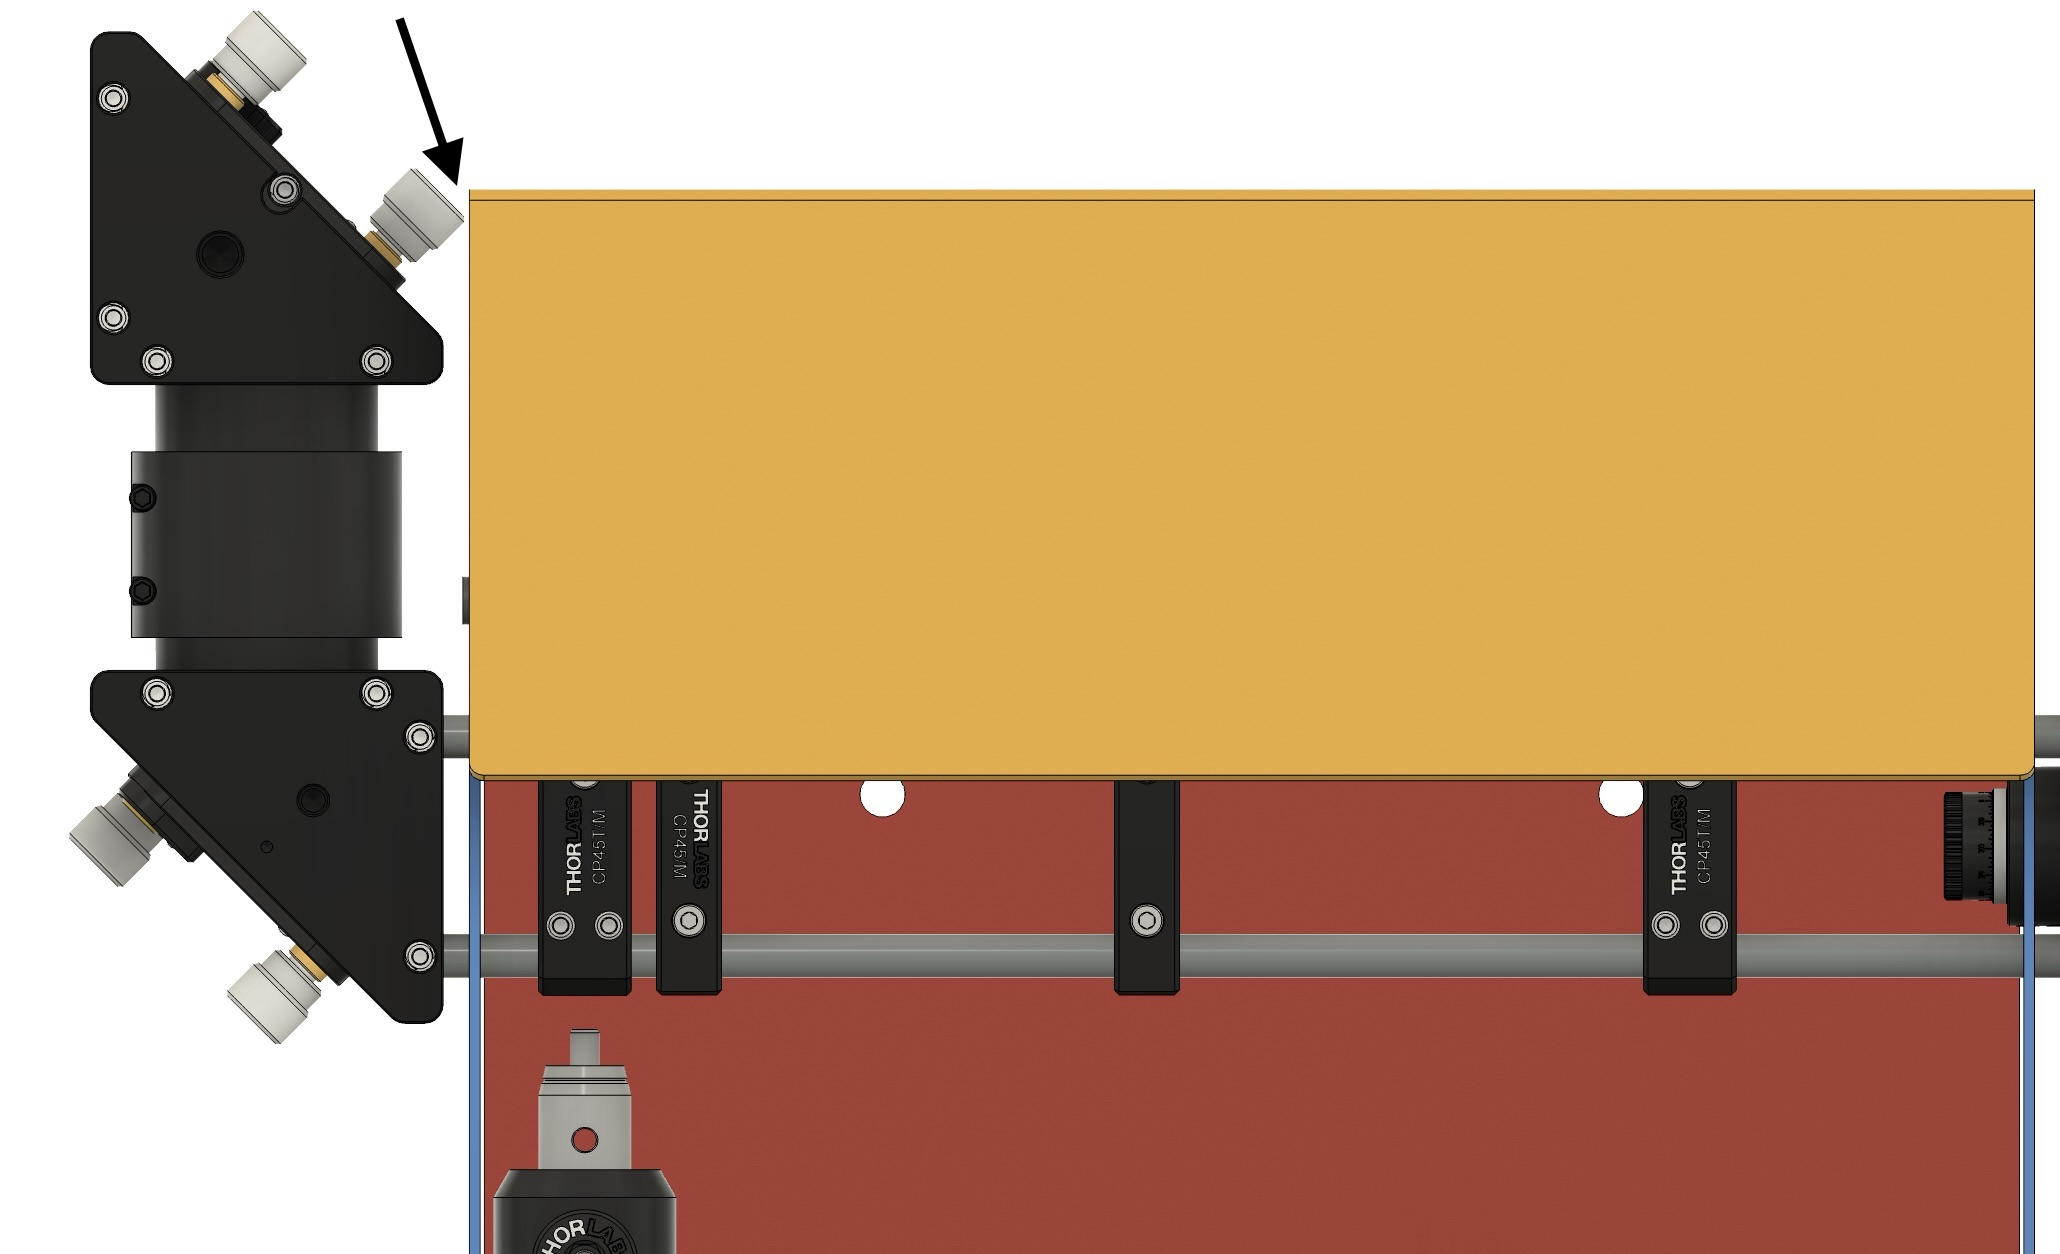
\includegraphics[width=\textwidth]{assets/figures/Protections_laser/Securite_mecanique/Protection_entree_laser/contrainte_vis.jpeg}
    \end{center}
    \captionof{figure}{Vue de face: Vis de réglage dans la course du capot supérieur}
    \label{contrainte_vis}
\end{minipage}

\begin{minipage}[c]{0.5\textwidth}
    La contrainte qui découle de la vis de réglage, et vu l'obligation de réduire la taille des protections, cela a créer un vide pouvant laisser passer les rayons du laser. Les traits manuscrits en rouge sur la Figure~\ref{contrainte_passage_laser_cage} représentent les fuites potentielles du laser. Ce phénomène apparaît également à droite des protections.

    La solution apportée a été d'ajouter un joint en mousse souple entourant les quatres axes qui formant la cage. Les protections viendraient s'appuyer sur les joints et combleraient les vides. Les détails en photo pour cette solution sont montrés à la section~\ref{prototype_bois}.
\end{minipage}\hfill
\begin{minipage}[c]{0.48\textwidth}
    \begin{center}
        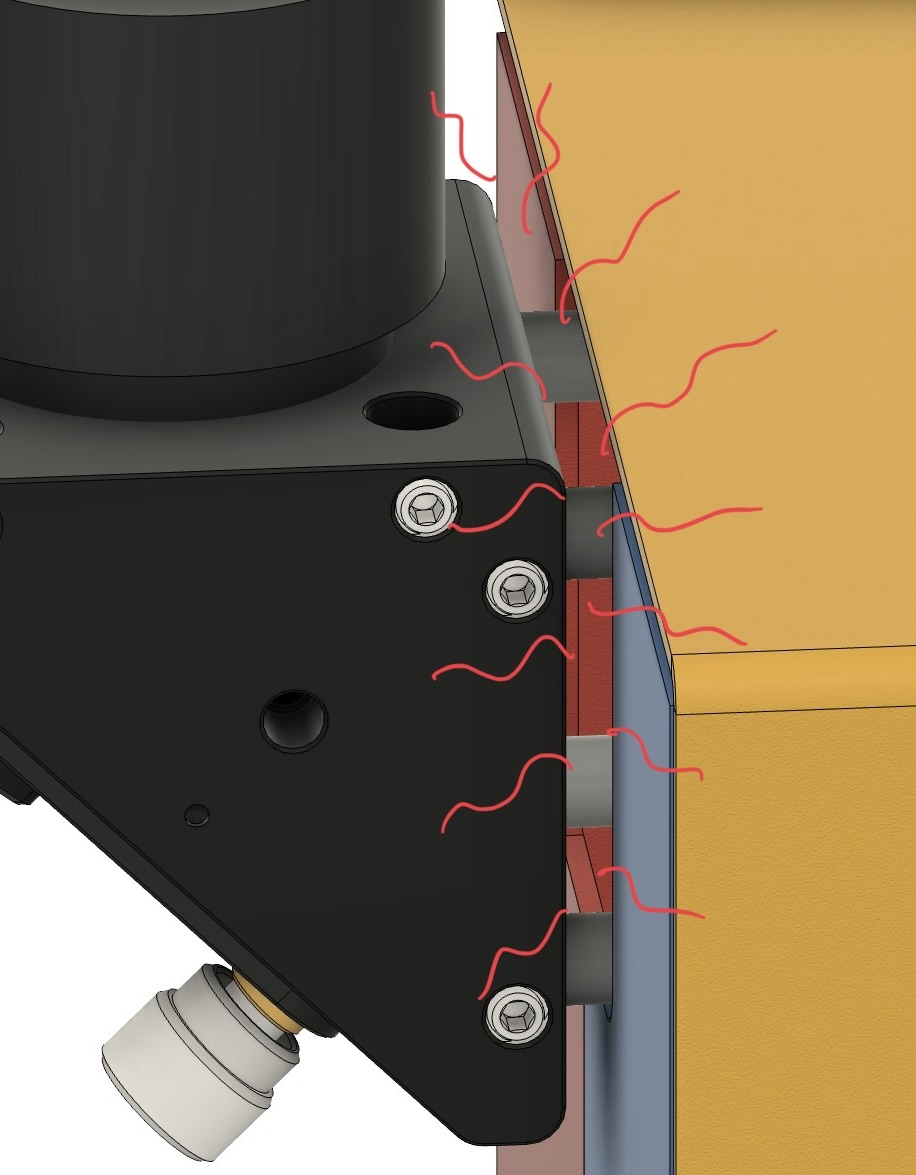
\includegraphics[width=0.9\textwidth]{assets/figures/Protections_laser/Securite_mecanique/Protection_entree_laser/contrainte_passage_laser_cage.jpeg}
    \end{center}
    \captionof{figure}{Vue en perspective cavalière: Fuites potentielles des rayons du laser pour les capots inférieurs}
    \label{contrainte_passage_laser_cage}
\end{minipage}

\begin{minipage}[c]{0.6\textwidth}
    La contrainte expliquée ici, similaire à la précédente, vient contrer les fuites possibles du laser. Cependant, cette fois, c'est pour la protection supérieure. En effet, lorsque le capot est fermé, il y'a un risque qu'il y ait des espaces fins où la lumière du faisceau peut s'échapper.

    La solution va également être la pose d'un joint, cette fois à l'intérieur du capot supérieur sur tout son contour. Ainsi, lorsque la protection est fermée, le joint va combler les vides. La modélisation ci-contre, voir la Figure~\ref{contrainte_passage_laser_capot}, montre qu'un espace entre la partie inférieure est supérieur de la protection a volontairement été créer afin de laisser de la place pour le joint.

    La solution apportée a été d'ajouter un joint en mousse souple entourant les quatres axes qui formant la cage. Les protections viendraient s'appuyer sur les joints et combleraient les vides. Les détails en photo pour cette solution sont montrés à la section~\ref{prototype_bois}.
\end{minipage}\hfill
\begin{minipage}[c]{0.38\textwidth}
    \begin{center}
        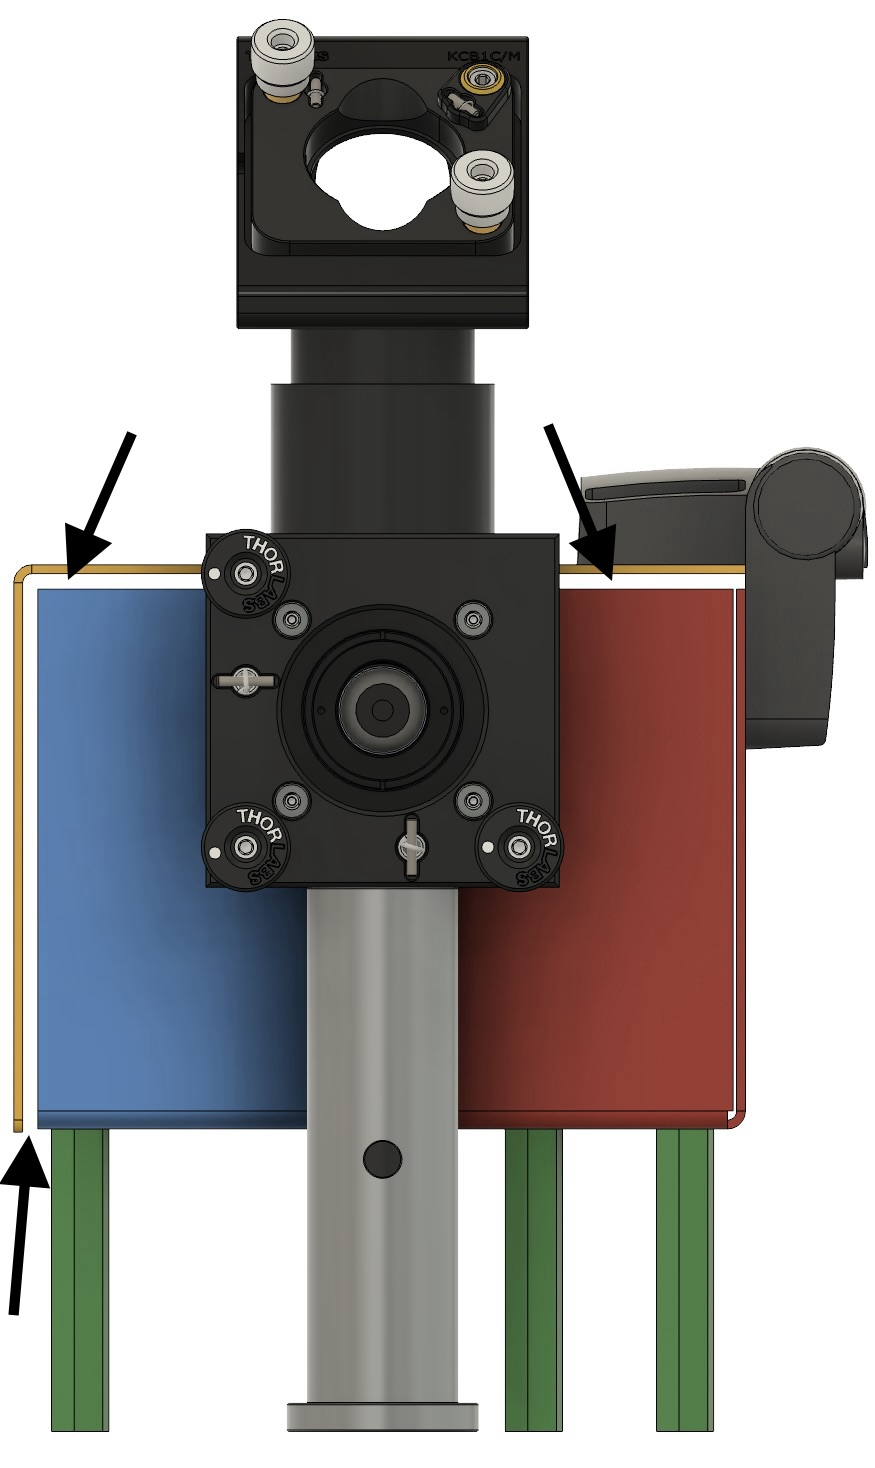
\includegraphics[width=\textwidth]{assets/figures/Protections_laser/Securite_mecanique/Protection_entree_laser/contrainte_passage_laser_capot.jpeg}
    \end{center}
    \captionof{figure}{Vue de droite: Fuites potentielles des rayons du laser pour le capot supérieur}
    \label{contrainte_passage_laser_capot}
\end{minipage}

\begin{minipage}{\textwidth}
    La dernière contrainte est: comment fixer les protections au kit ? Vu que la plaque de montage en aluminium, où sont fixés tous les composants du kit, contient des taraudages M6 sur toute sa surface, il est facile de trouver des encrages de fixation.

    La solution trouvée, illustrée ci-dessous sur la Figure~\ref{contrainte_entretoises}, est d'utiliser des entretoises. Deux pour fixer le capot inférieur avant, et trois pour le capot inférieur arrière. Ce dernier en contient plus, car subit plus de contraintes mécaniques. L'addition de la masse du capot inférieur arrière, de la charnière et du capot supérieur engendre un poid conséquent. Bien évidemment, il a fallu faire attention aux composants déjà positionnés et choisir judicieusement les emplacements des entretoises.

    Une entretoise hexagonale mesure 50~mm de hauteur, 8~mm de largeur et un taraudage M6 à chaque extrémité.

    Pour avoir une marge de sécurité, des oblongs ont été réalisés sur les tôles afin de faciliter leur fixation.
    \vspace{1em}
    \begin{center}
        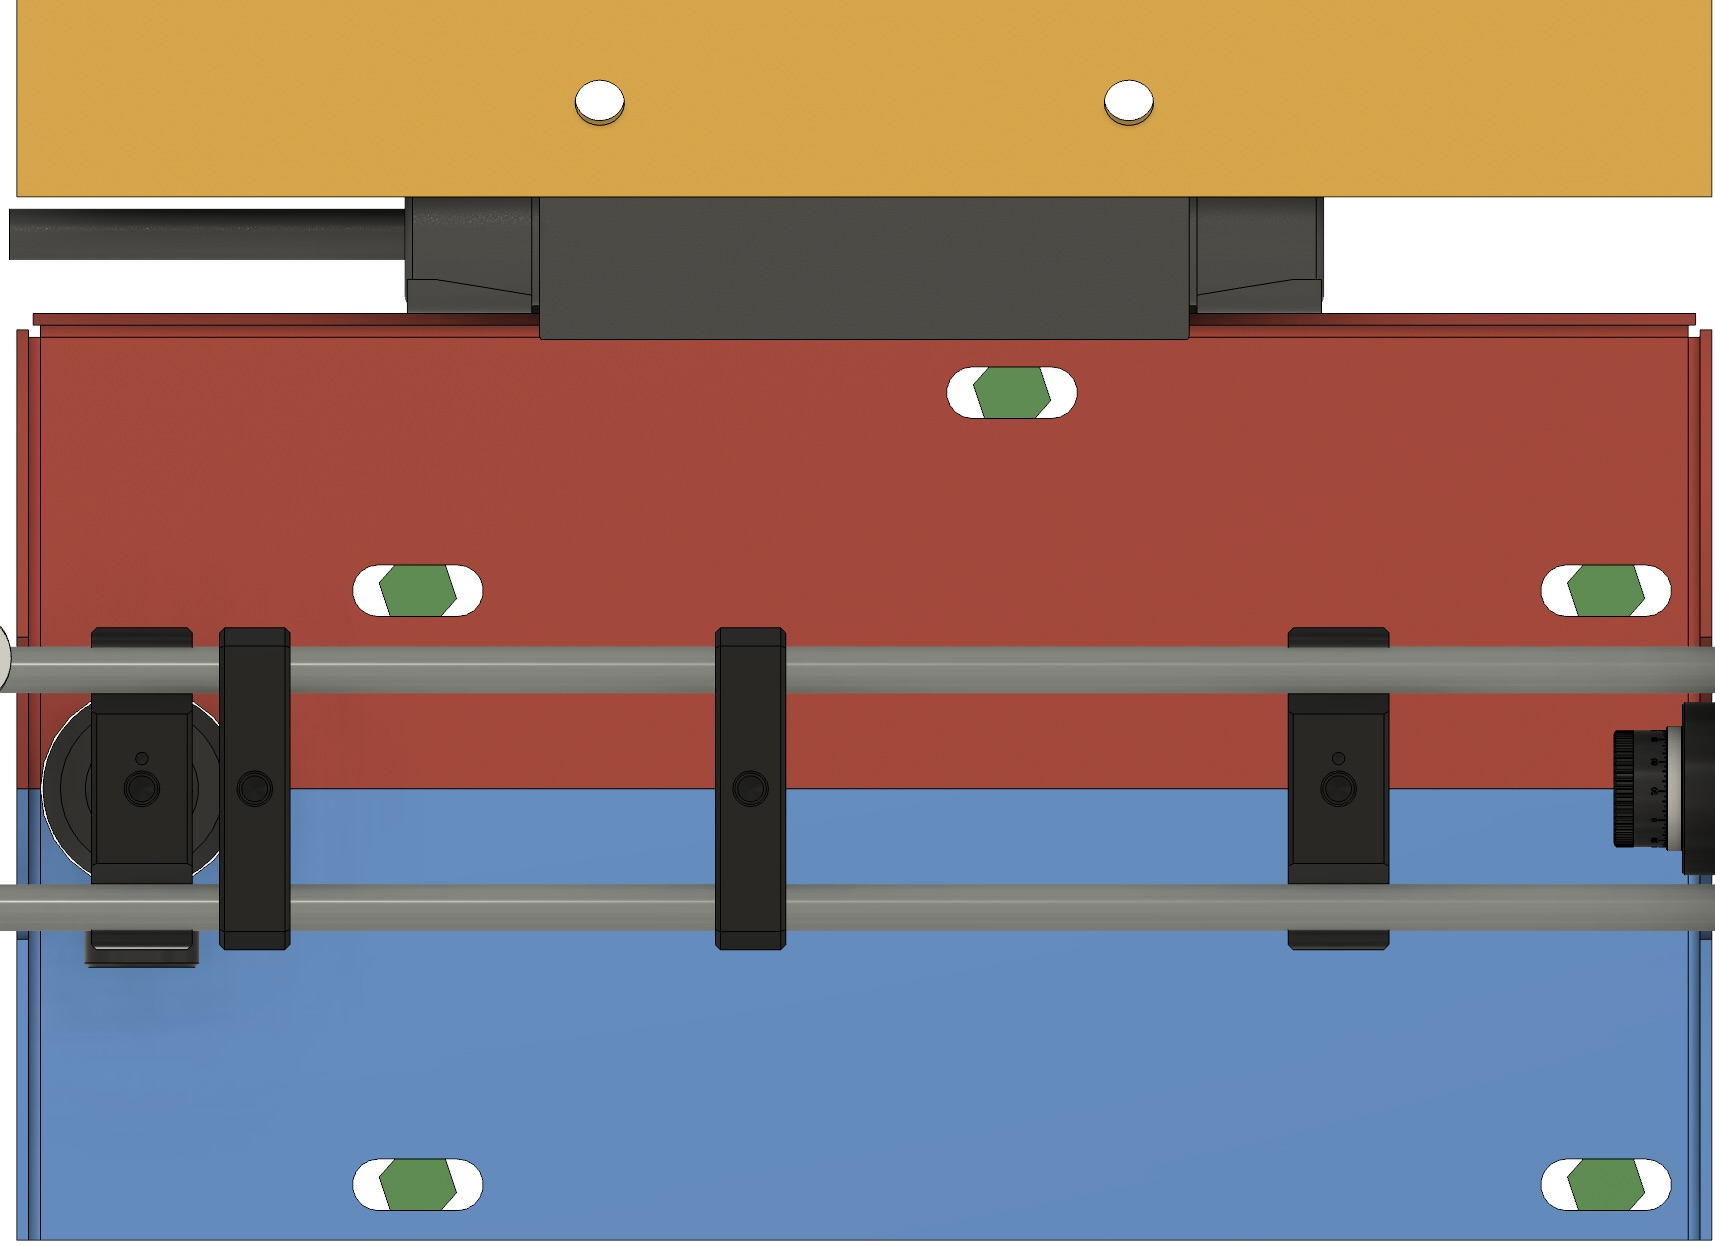
\includegraphics[width=0.7\textwidth]{assets/figures/Protections_laser/Securite_mecanique/Protection_entree_laser/contrainte_entretoises.jpeg}
    \end{center}
    \captionof{figure}{Vue de dessus: cinq entretoises pour fixer les capots au kit}
    \label{contrainte_entretoises}
\end{minipage}

\subsection{Mise en plan des pièces modélisées}
La modélisation terminée, il faut passer à la réalisation des dessins techniques pour la production des pièces. Une discussion préalable avec le responsable M. Ottonin, de l'atelier mécanique sur le site de Cheseaux, a eu lieu afin de parler du projet. Au cours de cet entretien, le matériau ainsi que l'épaisseur des différentes pièces a été choisi. Pour un usinage facile, le choix s'est porté sur l'aluminium avec une épaisseur de 1.5~mm. Les trois mises en plan se retrouvent au chapitre des annexes \ref{chapter:annexes}, sur les Figures~\ref{mise_en_plan_capot_avant},~\ref{mise_en_plan_capot_arriere}~e~\ref{mise_en_plan_capot_superieur}.

\begin{minipage}{\textwidth}
    \subsection{Réalisation d'un prototype en bois} \label{prototype_bois}
    Une fois les mises en plan faites, j'ai réalisé les trois pièces en MDF d'épaisseur 3~mm acheté chez Jumbo \cite{mdfJumbo}, afin d'être sûr des dimensions des pièces. Pour me faciliter la tâche, j'ai imprimer les dessins techniques à l'échelle~\texttt{1:1}, puis je les ai collés sur les panneaux en bois. Il ne restait plus qu'à découper les pièces au cutter. La Figure~\ref{decoupe_bois} illustre ces propos.
    \vspace{1em}
    \begin{center}
        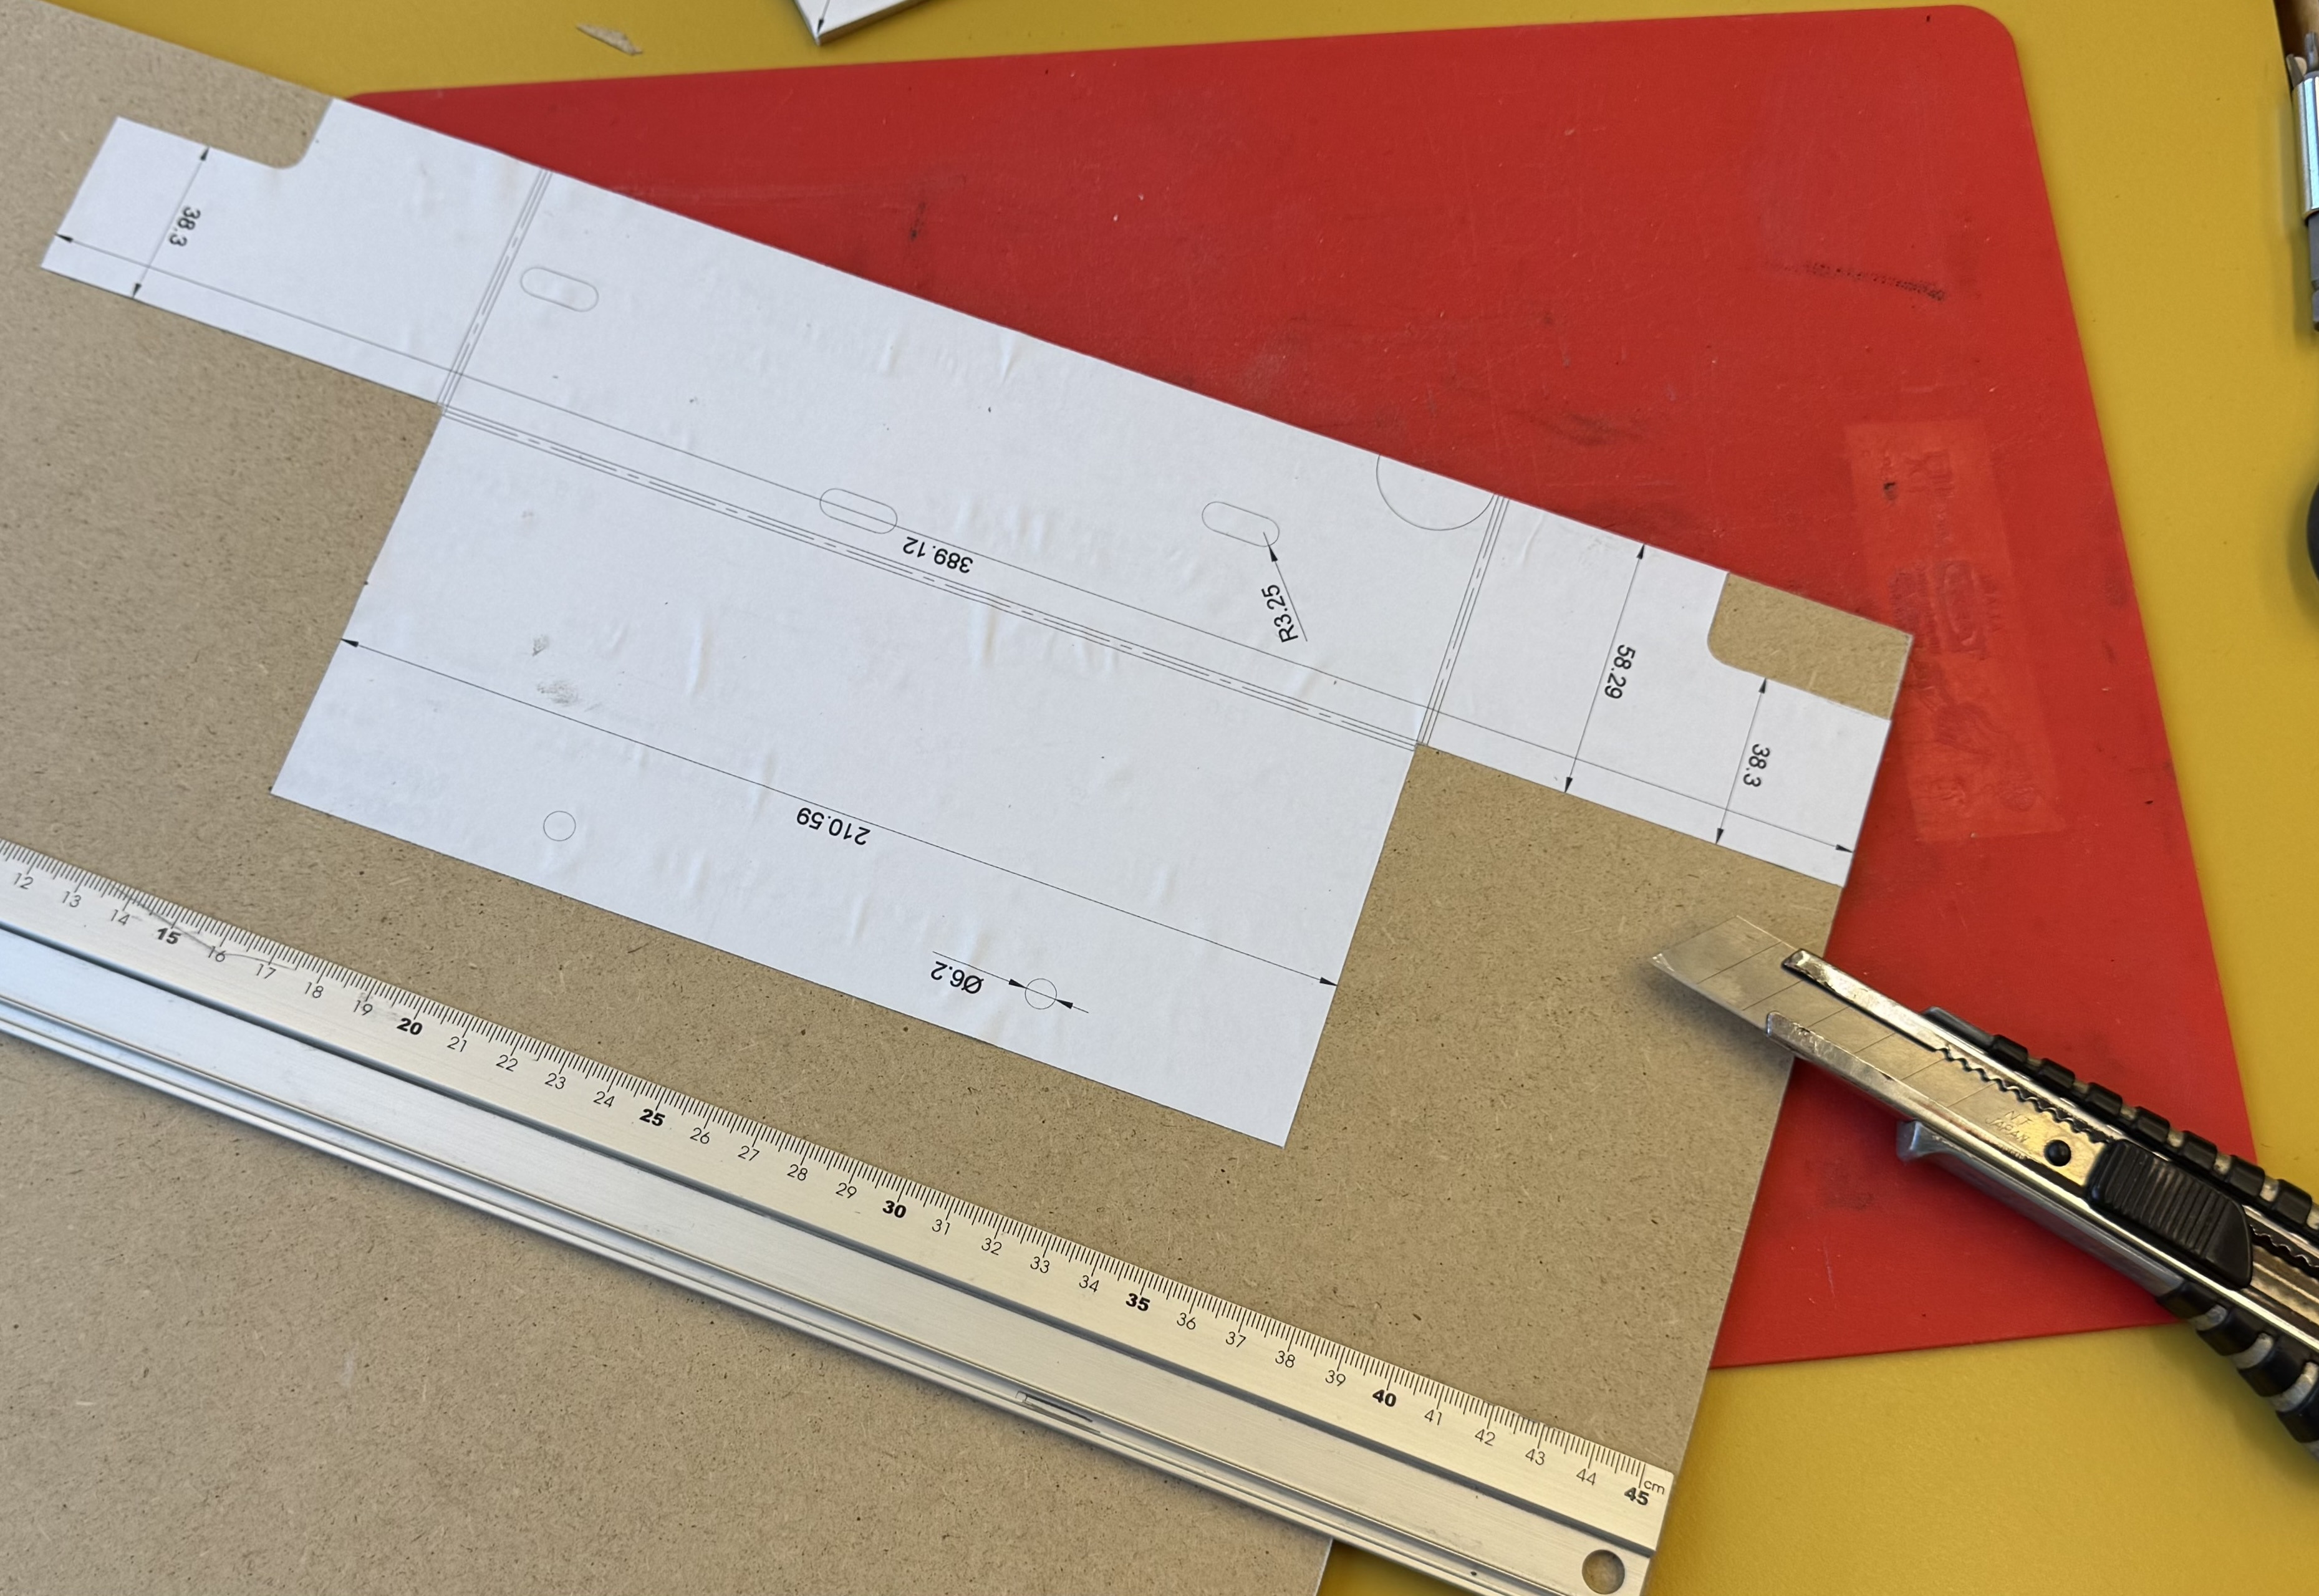
\includegraphics[width=0.8\textwidth]{assets/figures/Protections_laser/Securite_mecanique/Protection_entree_laser/decoupe_bois.jpeg}
    \end{center}
    \captionof{figure}{Découpe des protections en bois à l'aide des plans imprimés}
    \label{decoupe_bois}
\end{minipage}

\begin{minipage}{\textwidth}
    Pour tenir les différents pliages, des carelets en bois ont été fixés, montrés par les flèches noires sur la Figure~\ref{montage_bois}.

    La fèche \textcolor{red}{rouge} montre le joint qui empêche les rayons du laser de passer outre la protection. Le joint a une épaisseur de 3~mm au repos.
    \vspace{1em}
    \begin{center}
        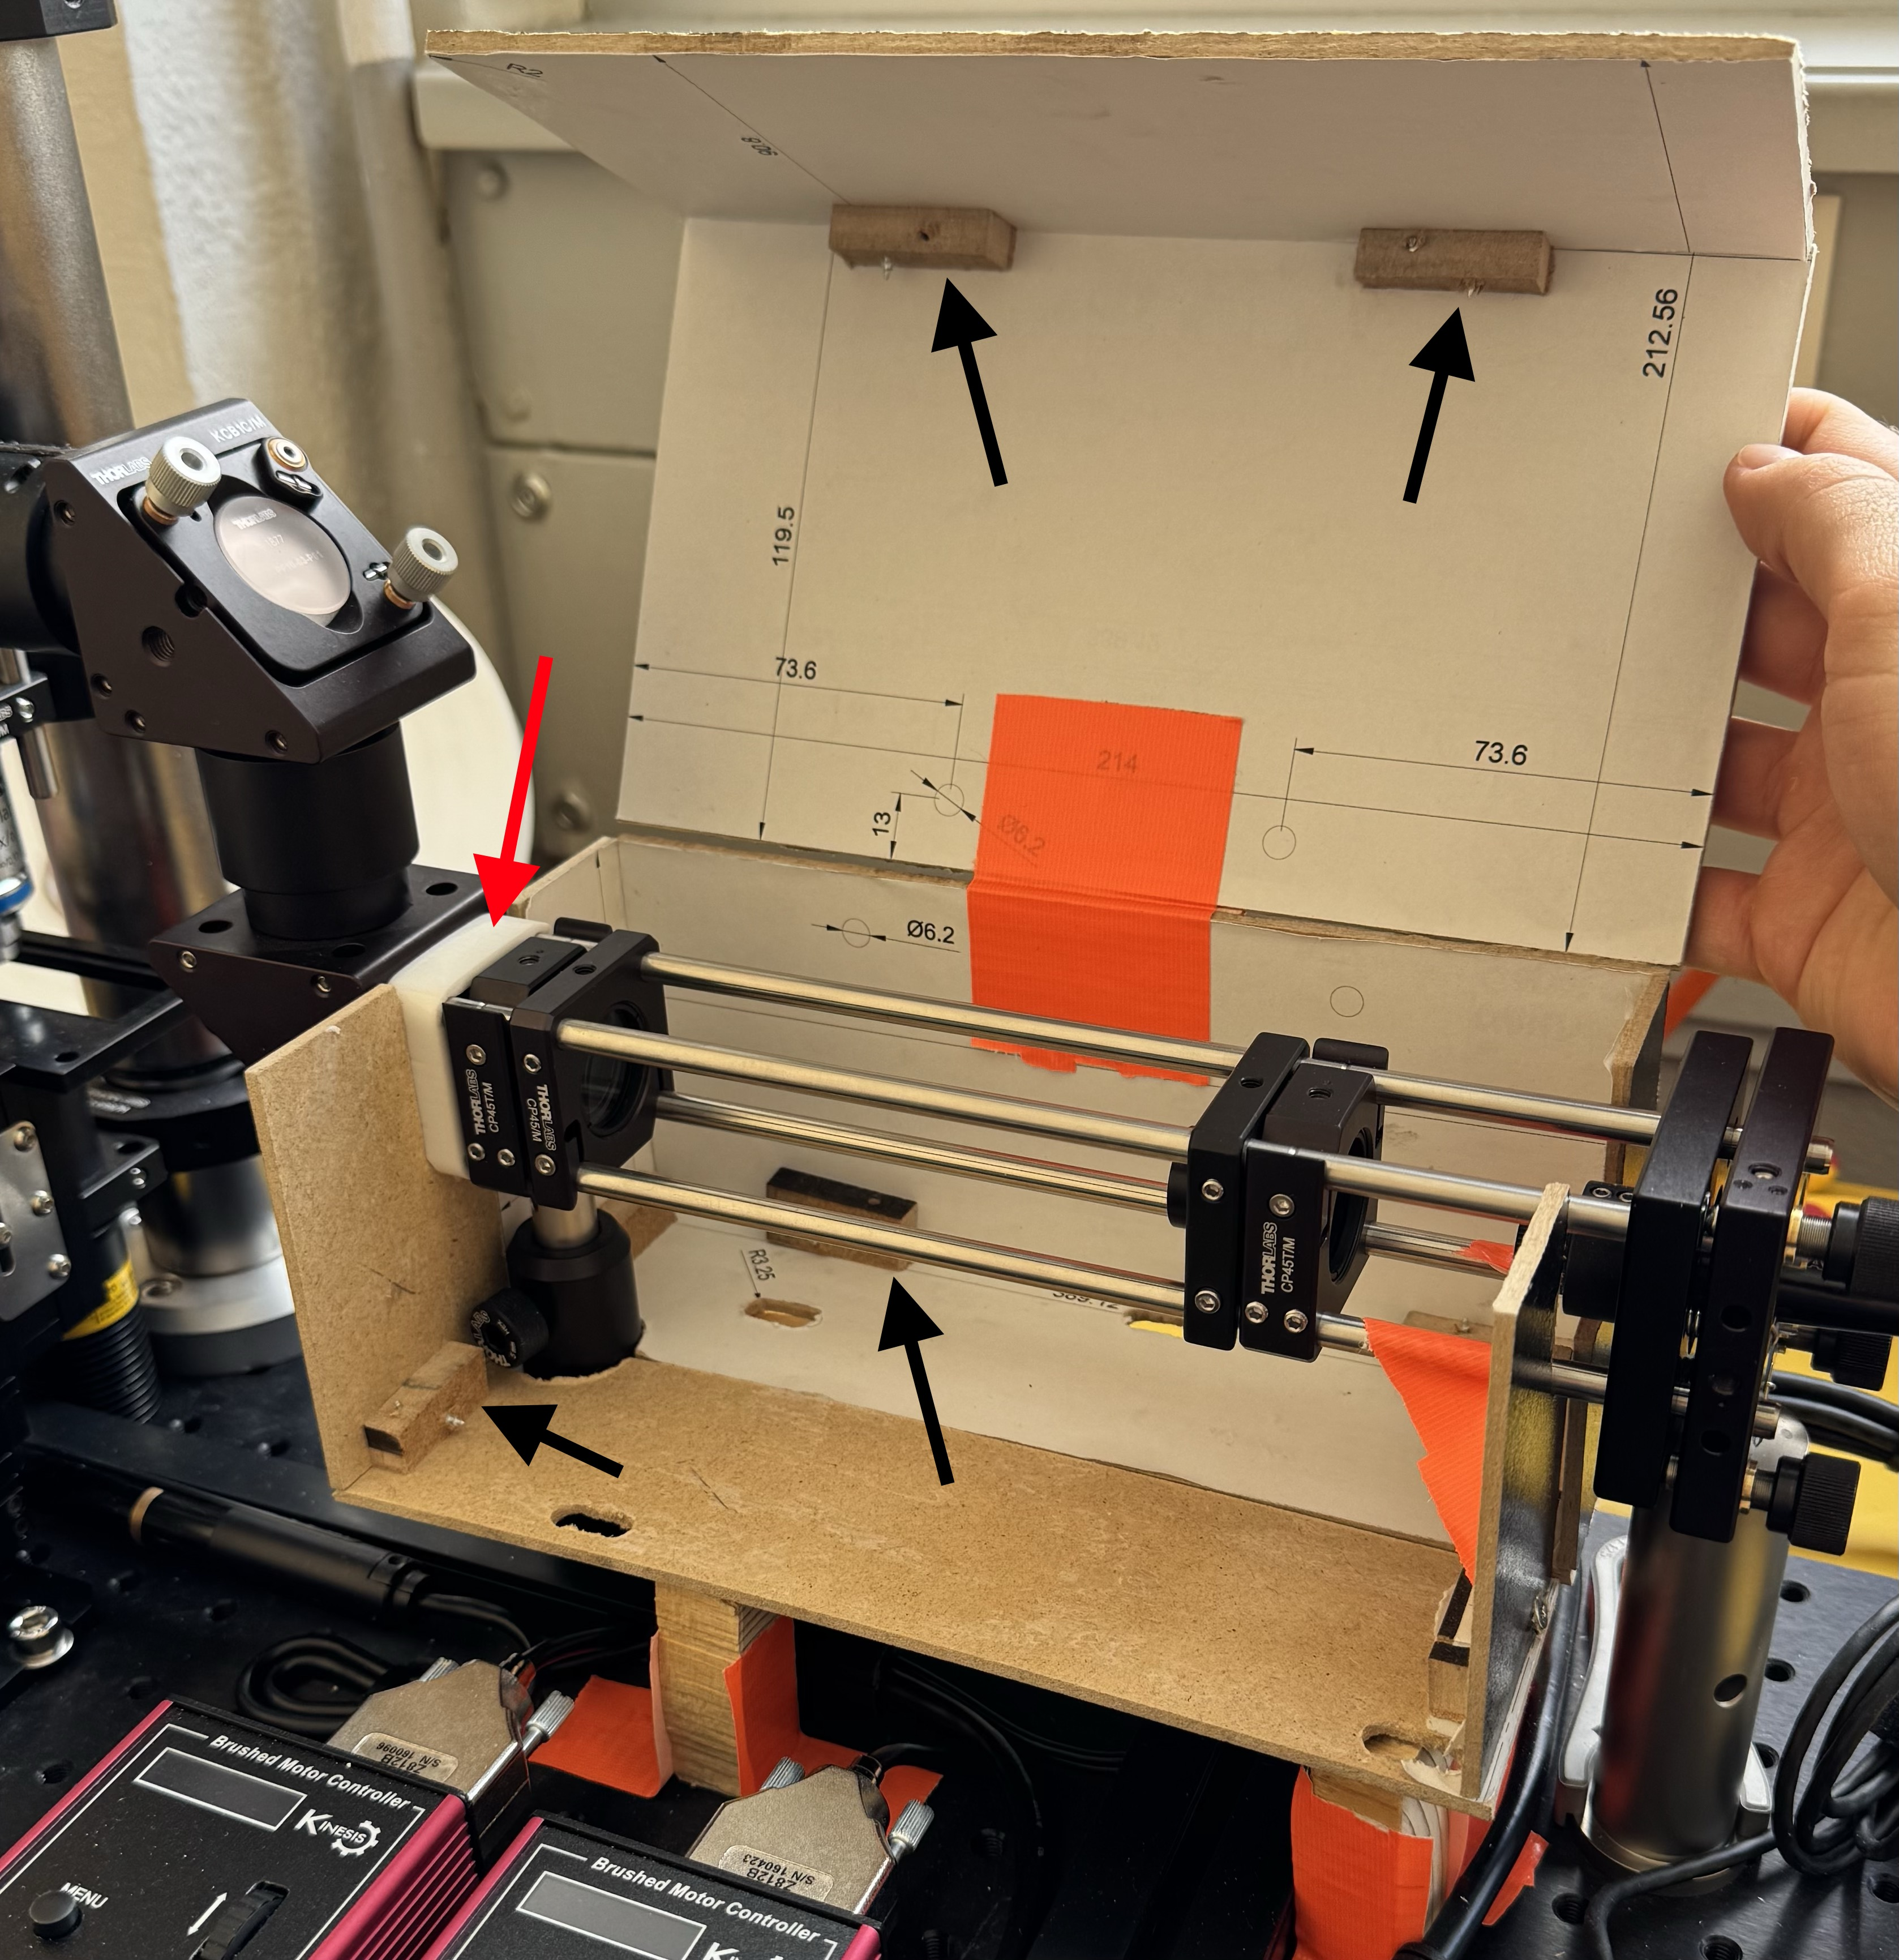
\includegraphics[width=0.6\textwidth]{assets/figures/Protections_laser/Securite_mecanique/Protection_entree_laser/montage_bois.jpeg}
    \end{center}
    \captionof{figure}{Montage de la protection à l'entrée du laser en bois MDF de 3~mm}
    \label{montage_bois}
\end{minipage}
\subsection{Fabrication des pièces en aluminium}
\begin{minipage}{\textwidth}

    \begin{minipage}[c]{0.6\textwidth}
        La Figure~\ref{capots_brutes} ci-contre, montre les trois pièces usinées par l'atelier mécanique, telles que reçues. Une peinture noire mat vient recouvrir les pièces pour absorber les rayons du laser.
    \end{minipage}\hfill
    \begin{minipage}[c]{0.35\textwidth}
        \begin{figure}[H]
            \centering
            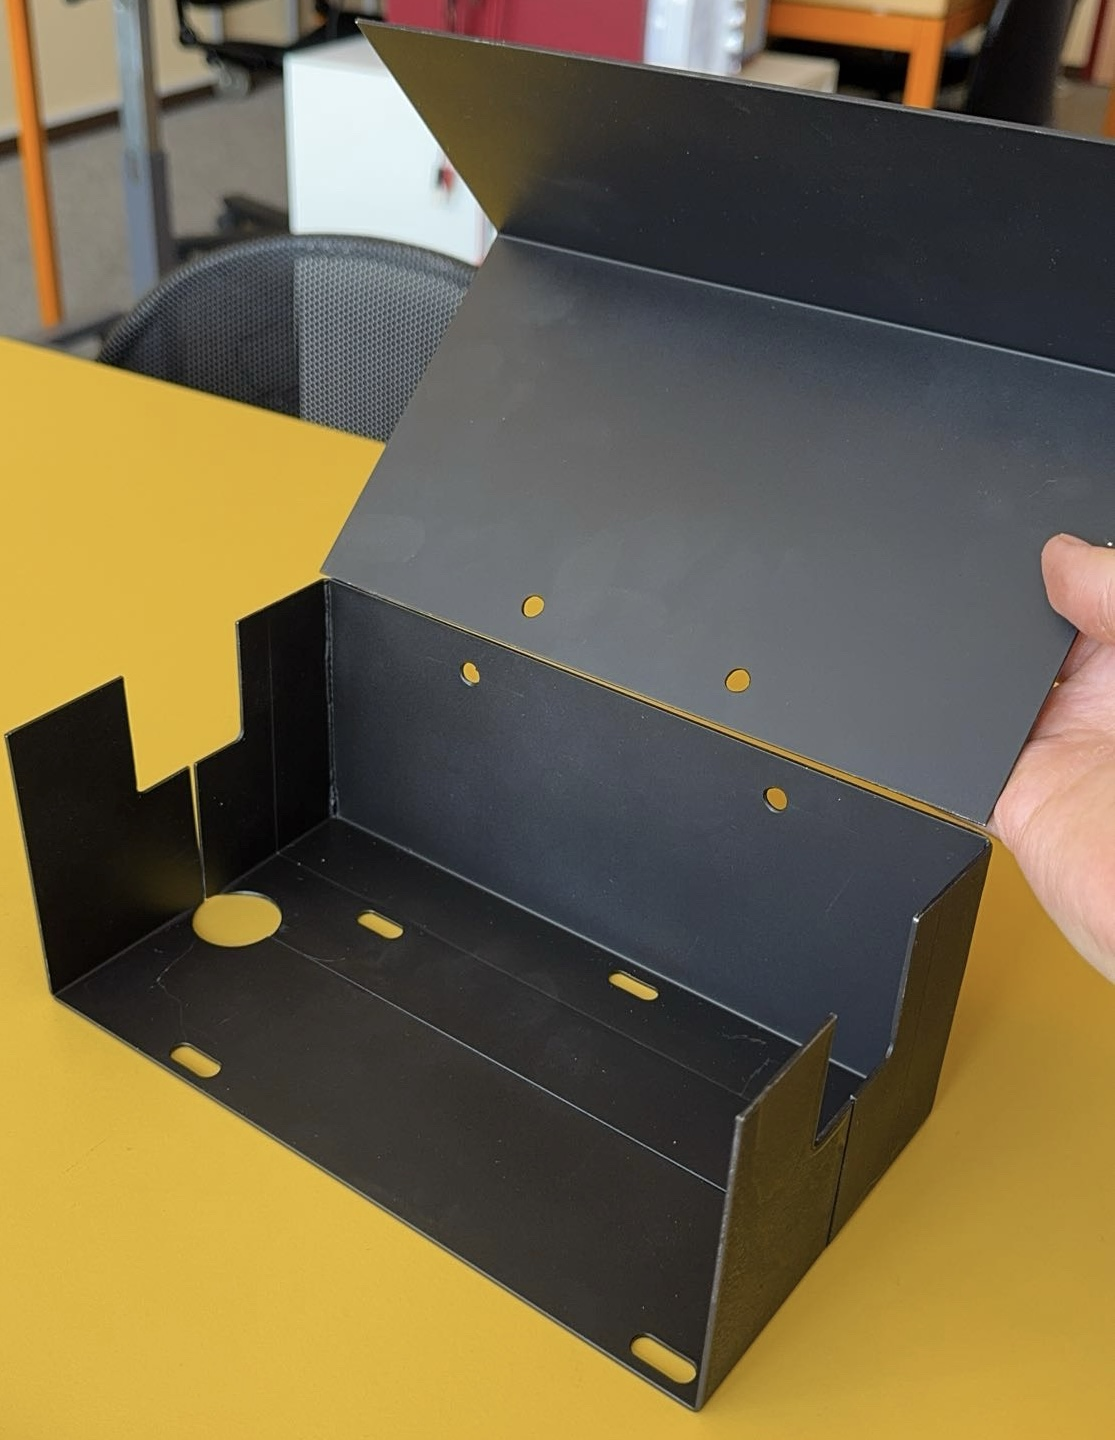
\includegraphics[width=\textwidth]{assets/figures/Protections_laser/Securite_mecanique/Protection_entree_laser/capots_brutes.jpg}
            \caption{Les trois protections fabriquées en aluminium 1.5~mm d'épaisseur}
            \label{capots_brutes}
        \end{figure}
    \end{minipage}
\end{minipage}


\begin{minipage}{\textwidth}
    \subsection{Montage final}
    Les figures~\ref{montage_alu_ouvert}~et~\ref{montage_alu_ferme} ci-dessous, montre le montage final des trois capots sur le kit.
    \vspace{1em}

    \begin{minipage}[c]{0.48\textwidth}
        \begin{figure}[H]
            \begin{center}
                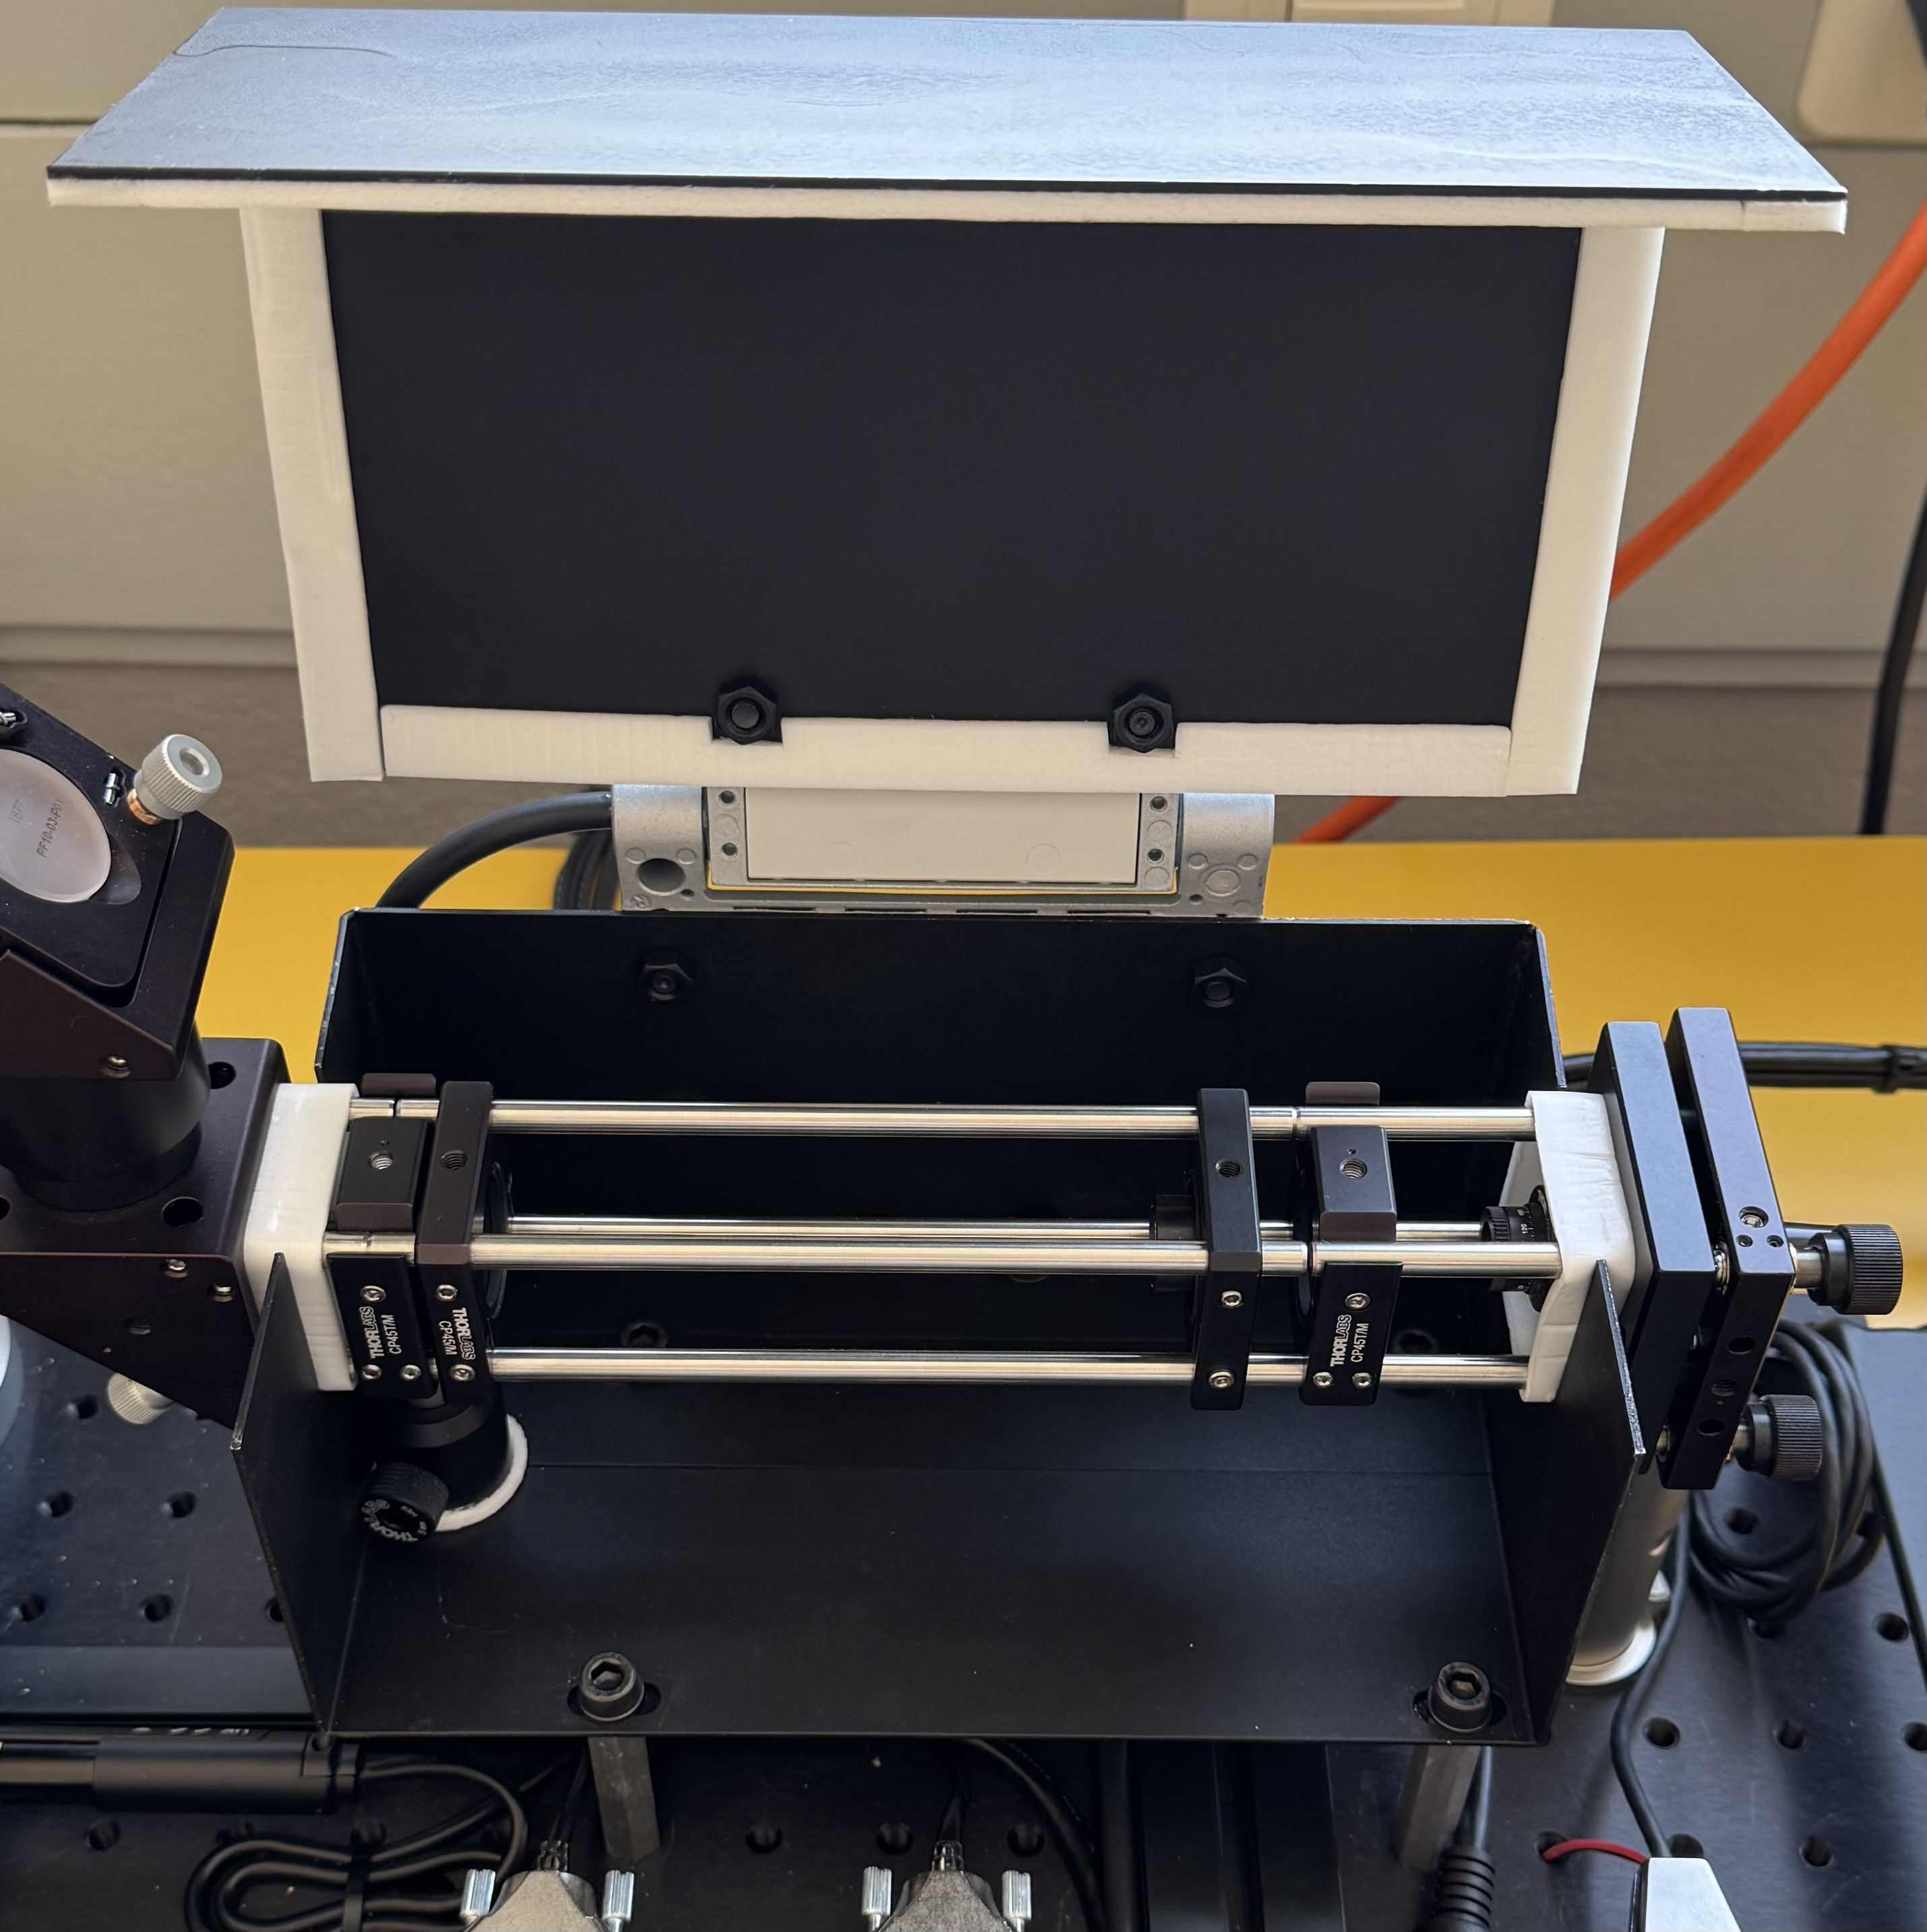
\includegraphics[height=6cm]{assets/figures/Protections_laser/Securite_mecanique/Protection_entree_laser/montage_alu_ouvert.jpeg}
            \end{center}
            \captionof{figure}{Montage de la protection en aluminium ouvert}
            \label{montage_alu_ouvert}
        \end{figure}
    \end{minipage}
    \begin{minipage}[c]{0.48\textwidth}
        \begin{figure}[H]
            \begin{center}
                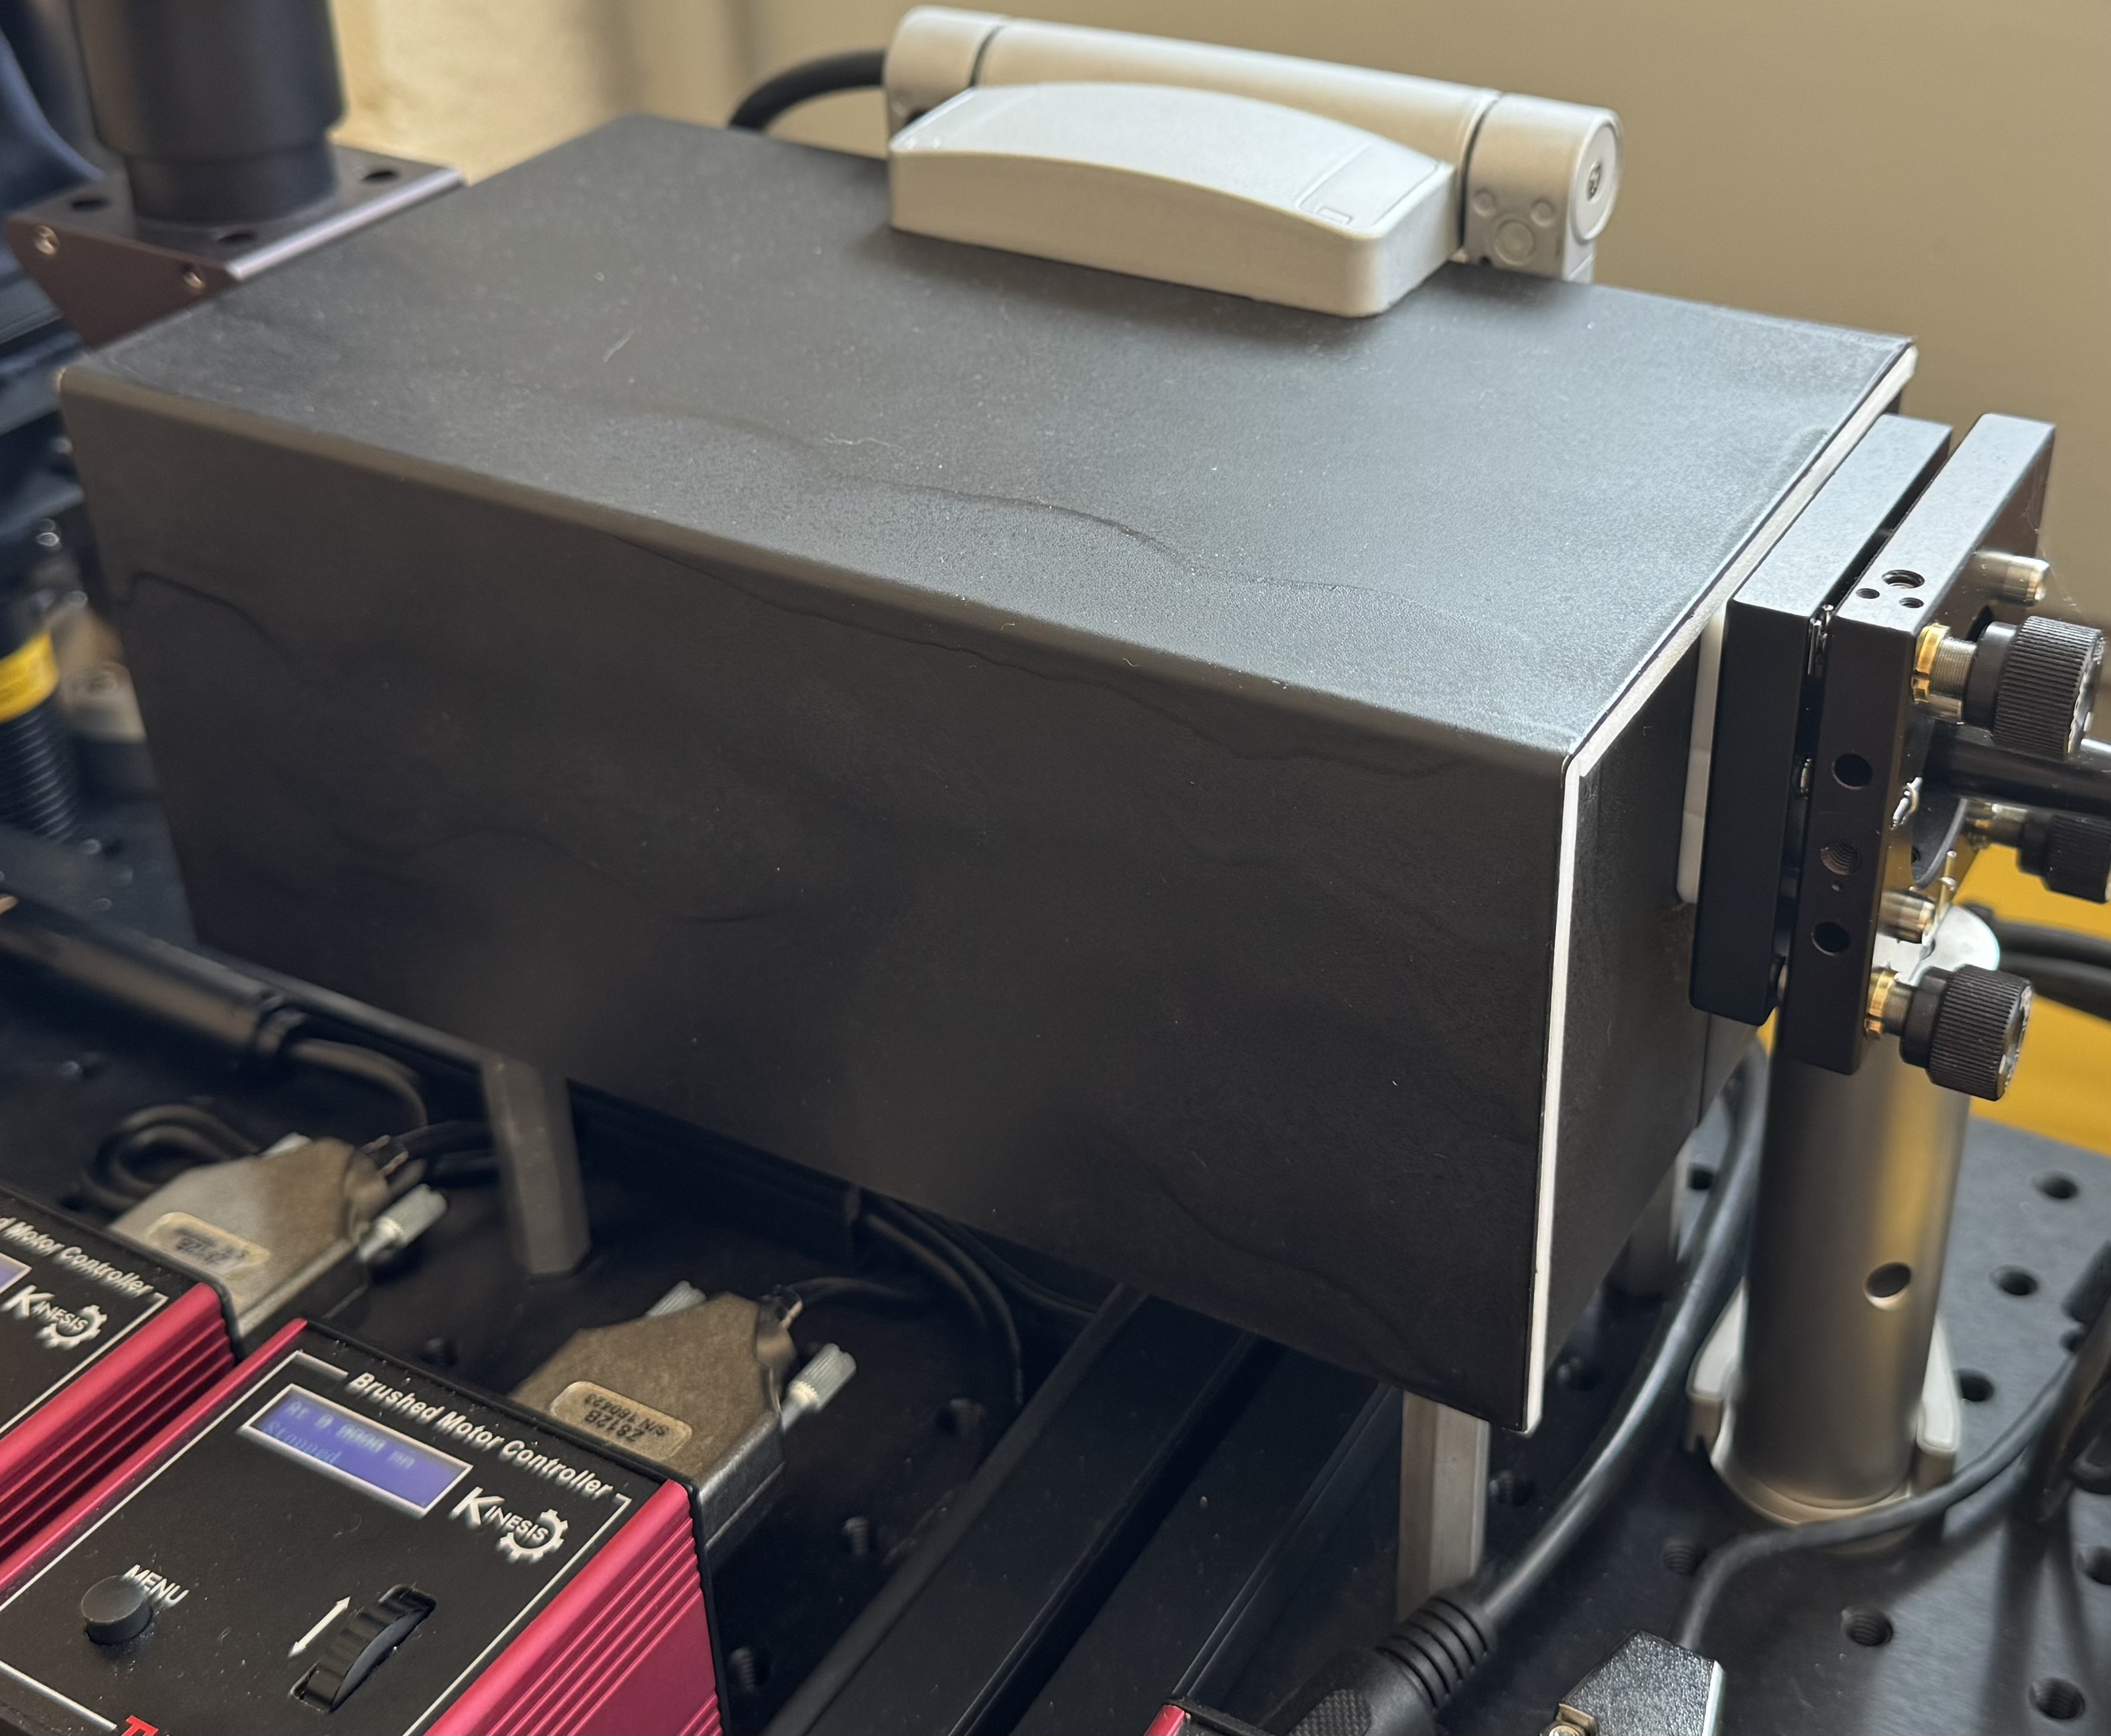
\includegraphics[height=6cm]{assets/figures/Protections_laser/Securite_mecanique/Protection_entree_laser/montage_alu_ferme.jpeg}
            \end{center}
            \captionof{figure}{Montage de la protection en aluminium fermé}
            \label{montage_alu_ferme}
        \end{figure}
    \end{minipage}
\end{minipage}

\begin{minipage}{\textwidth}
    Le tableau~\ref{tab:visserie_protection} récapitule toute la visserie nécessaires pour le montage des protections sur le kit.
    \begin{table}[H]
        \centering
        \renewcommand{\arraystretch}{1.3}
        \begin{tabular}{|l|c|l|}
            \hline
            \textbf{Élément} & \textbf{Quantité} & \textbf{Utilisation}                                   \\
            \hline
            Vis CHC M6x20    & 5                 & Fixation des entretoises à la plaque de montage en alu \\
            Vis CHC M6x8     & 5                 & Fixation des tôles sur les entretoises                 \\
            Rondelles M6     & 5                 & Avec les vis M6x8                                      \\
            Vis CHC M6x16    & 4                 & Fixation de la charnière aux tôles                     \\
            Écrous M6        & 4                 & Pour les vis de la charnière                           \\
            \hline
        \end{tabular}
        \caption{Visserie nécessaire au montage de la protection}
        \label{tab:visserie_protection}
    \end{table}
\end{minipage}
\subsection{Points d'améliorations}
\begin{enumerate}
    \item Les oblongs ne sont pas nécessaires. Au montage, je me suis rendu compte qu'en vissant les protections, la rondelle ne couvrait pas entièrement les oblongs. De ce fait, il y'avait un jour. J'ai ajouter du scotch noir afin de combler ces trous.
    \item La conception de la protection peut sûrement être améliorée. Par exemple il serait peut être possible de réduire le nombre de fixations, afin de gagner en ergonomie.
\end{enumerate}
\clearpage
\section{Protection vers le microscope}
Cette section va expliquer les différentes étapes de la conception de la protection vers le microscope, la
modélisation de celle-ci, les prototypes qui ont été réalisés, la fabrication final ainsi
que le montage.
\subsection{Réflexion préliminaire}
Contrairement à la précédente protection, la table croisée bouge dans l'espace sur les trois axes X,Y et Z. Il faut, dans ce cas, trouvé un moyen de faire une protection qui puisse être mobile afin de supporter les efforts dans toutes les directions. La table peut se déplacer d'environ 12~mm en X et Y, et de 25~mm en Z.

La première approche s'est tournée vers de l'impression 3D de plastique souple, tel que du TPU. Ses propriétés élastiques permettent d'avoir une certaine liberté de mouvement.

Les Figures~\ref{zigzag_model}~et~\ref{zigzag_reel} ci-dessous, illustrent un modèle 3D de test avec une géométrie en \textit{zigzag}, afin de tester ses propriétés élastiques. Ce modèle n'a pas du tout été concluant, la structure est beaucoup trop rigide en élasticité et au contraire.

\begin{minipage}[c]{0.48\textwidth}
    \begin{center}
        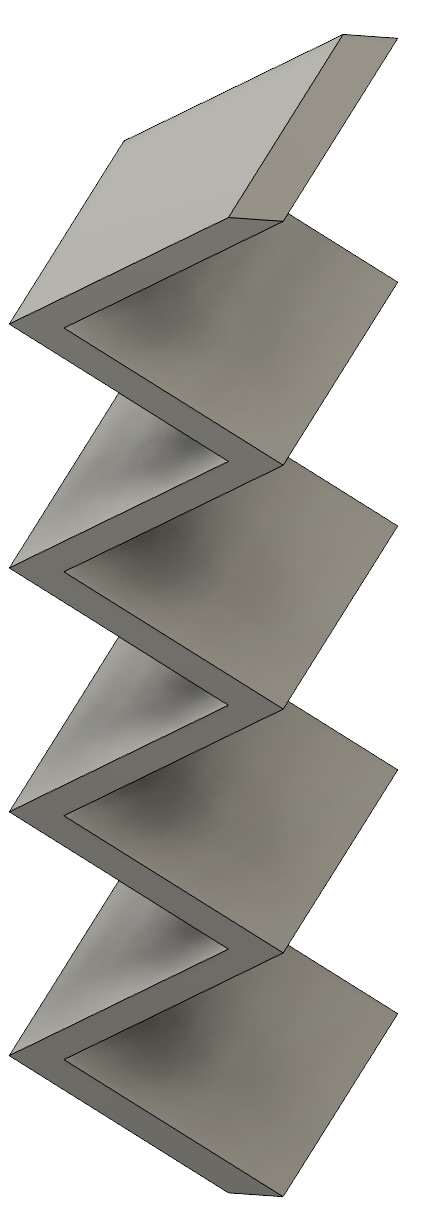
\includegraphics[width=0.2\textwidth]{assets/figures/Protections_laser/Securite_mecanique/Protection_vers_microscope/zigzag_model.jpeg}
    \end{center}
    \captionof{figure}{Modèle 3D avec géométrie en zigzag}
    \label{zigzag_model}
\end{minipage}\hfill
\begin{minipage}[c]{0.48\textwidth}
    \begin{center}
        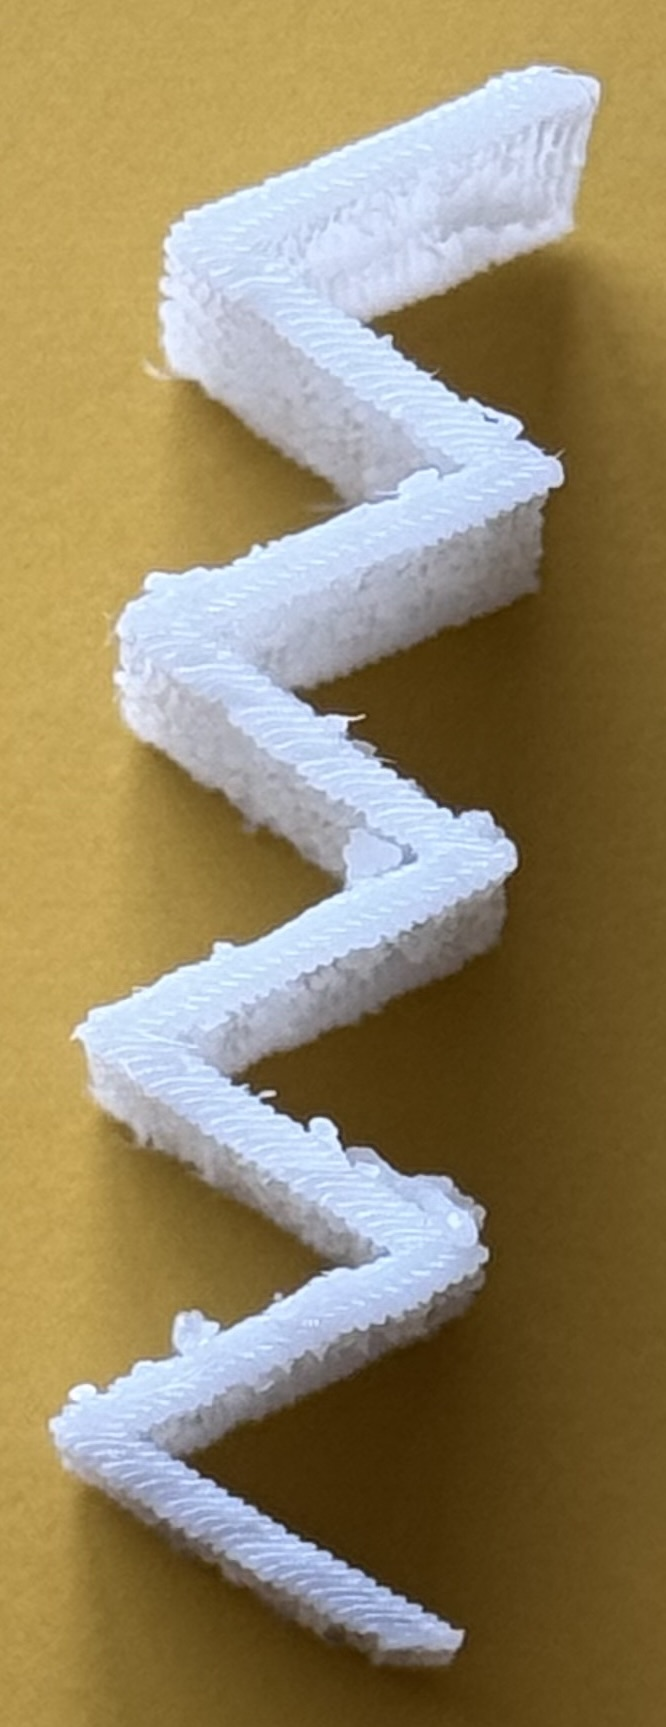
\includegraphics[width=0.2\textwidth]{assets/figures/Protections_laser/Securite_mecanique/Protection_vers_microscope/zigzag_reel.jpeg}
    \end{center}
    \captionof{figure}{Impression 3D en TPU du modèle avec géométrie en zigzag}
    \label{zigzag_reel}
\end{minipage}

La solution retenu pour avoir le moins de contraintes possible dans les mouvements a été de faire une conception de protection avec du tissu, associée à des impressions 3D en PLA.

\subsection{Modélisation de la protection}
\begin{minipage}[c]{0.38\textwidth}
    Pour pouvoir mieux comprendre les choix de conception et les étapes faites pour réaliser la protection, la Figure~\ref{model_3D_microscope}, ci-contre, représente la modélisation complète de la protection vers le microscope. Les modélisation crées pour cette protection sont en couleur sur la représentation 3D.
\end{minipage}\hfill
\begin{minipage}[c]{0.58\textwidth}
    \begin{center}
        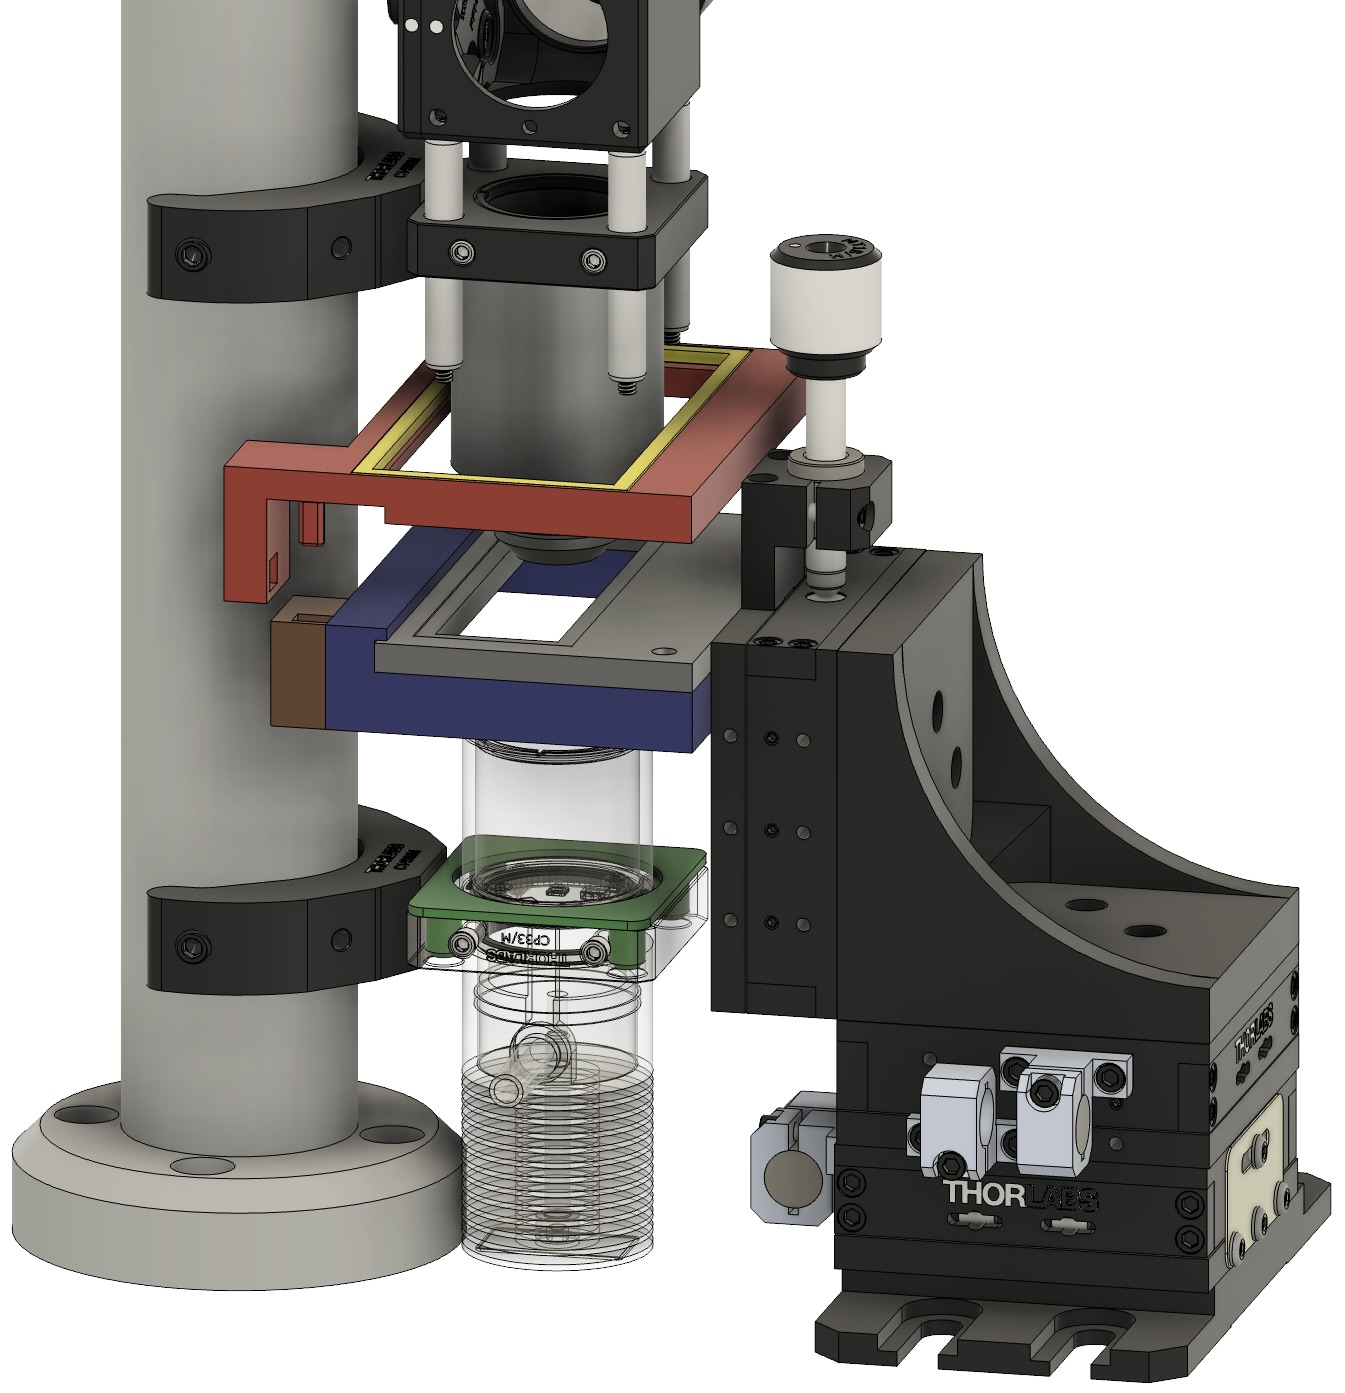
\includegraphics[width=\textwidth]{assets/figures/Protections_laser/Securite_mecanique/Protection_vers_microscope/model_3D.jpeg}
    \end{center}
    \captionof{figure}{Modèle 3D complet de la protection vers le microscope}
    \label{model_3D_microscope}
\end{minipage}

\begin{table}[H]
    \centering
    \caption{Nomenclature des pièces modélisées avec code couleur pour la protection vers le microscope}
    \begin{tabular}{|c|l|}
        \hline
        \textbf{Couleur}                         & \textbf{Nom de la pièce}                             \\
        \hline
        \multicolumn{2}{|c|}{\textbf{Partie inférieure}}                                                \\
        \hline
        \textcolor[RGB]{70, 170, 70}{Vert}       & Support pour fixer le tissu inférieur à la LED       \\
        \textcolor[RGB]{30, 50, 150}{Bleu foncé} & Support pour fixer le tissu inférieur à la platine   \\
        \hline
        \multicolumn{2}{|c|}{\textbf{Partie supérieure}}                                                \\
        \hline
        \textcolor[RGB]{170, 50, 50}{Rouge}      & Support clipsable sur la platine                     \\
        \textcolor[RGB]{120, 70, 30}{Brun}       & Boîtier pour fixer le fin de course                  \\
        \textcolor[RGB]{233, 173, 56}{Jaune}     & Cadre pour fixer le tissu supérieur au support rouge \\
        \hline
    \end{tabular}
    \label{tab:nomenclature_pieces_microscope}
\end{table}

\subsubsection{Partie inférieure}
\begin{minipage}[c]{0.48\textwidth}
    Pour fixer le tissu à LED (pièce \textcolor[RGB]{70, 170, 70}{verte} de la Figure~\ref{model_3D_microscope}), le support montré sur la Figure~\ref{support_inf_tissu_LED}, ci-contre, a été pensé. La plaque, désigné par la flèche \textcolor{red}{rouge}, est une plaque de cage.
    \vspace{1em}
    Ses quatres trous ont été utilisés pour pouvoir fixer le support. les quatres petites vis (flèches \textcolor[RGB]{115, 210, 210}{bleues}), sont des vis sans têtes pour serrer le support en place. Le tissu est pincé entre la plaque et le support imprimé.
\end{minipage}\hfill
\begin{minipage}[c]{0.48\textwidth}
    \begin{center}
        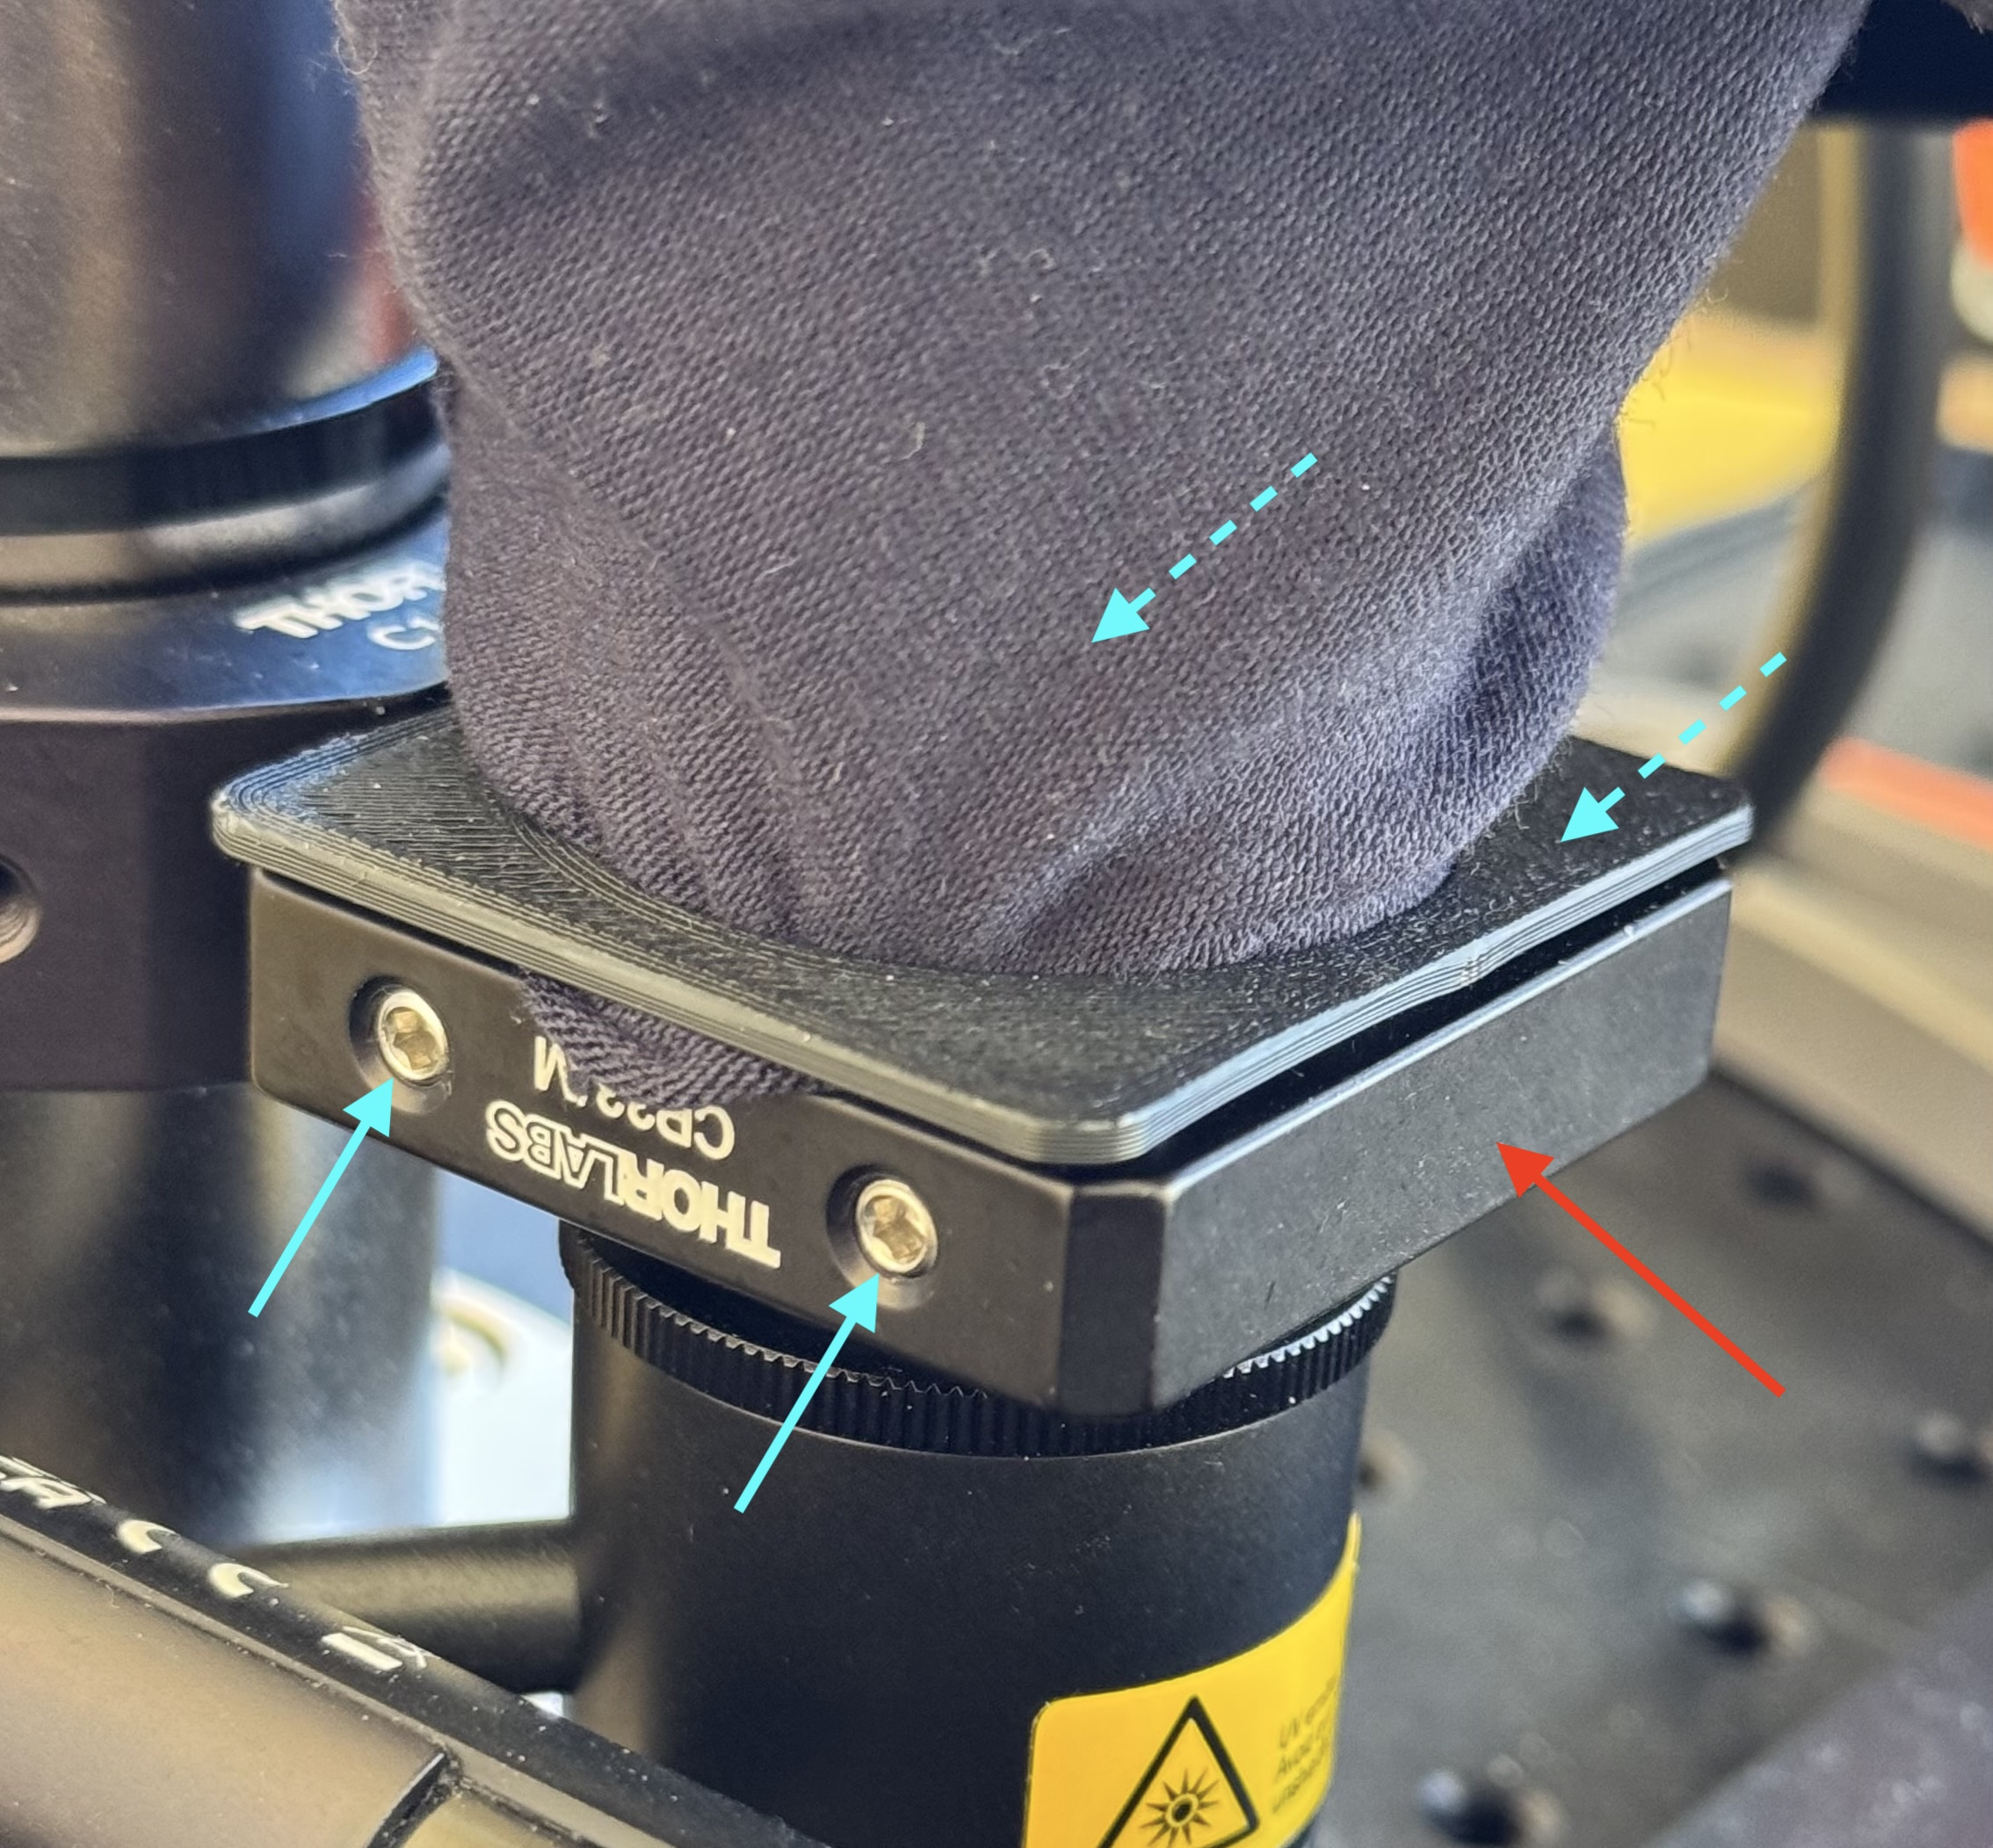
\includegraphics[width=0.9\textwidth]{assets/figures/Protections_laser/Securite_mecanique/Protection_vers_microscope/support_inf_tissu_LED.jpeg}
    \end{center}
    \captionof{figure}{Support pour fixer le tissu inférieur à la lED}
    \label{support_inf_tissu_LED}
\end{minipage}

\begin{minipage}[c]{0.48\textwidth}
    Pour fixer le tissu à la platine (pièce \textcolor[RGB]{30, 50, 150}{bleu foncé} de la Figure~\ref{model_3D_microscope}), le support montré sur la Figure~\ref{support_inf_tissu_platine} (flèche \textcolor{red}{rouge}), ci-contre, a été élaboré.

    \vspace{1em}
    Pour le fixer, les vis montrées par les flèches \textcolor[RGB]{115, 210, 210}{bleues} ont été utilisées. Comme pour la fixation à la LED, ici, le tissu est également coincé entre la platine et le support.
\end{minipage}\hfill
\begin{minipage}[c]{0.48\textwidth}
    \begin{center}
        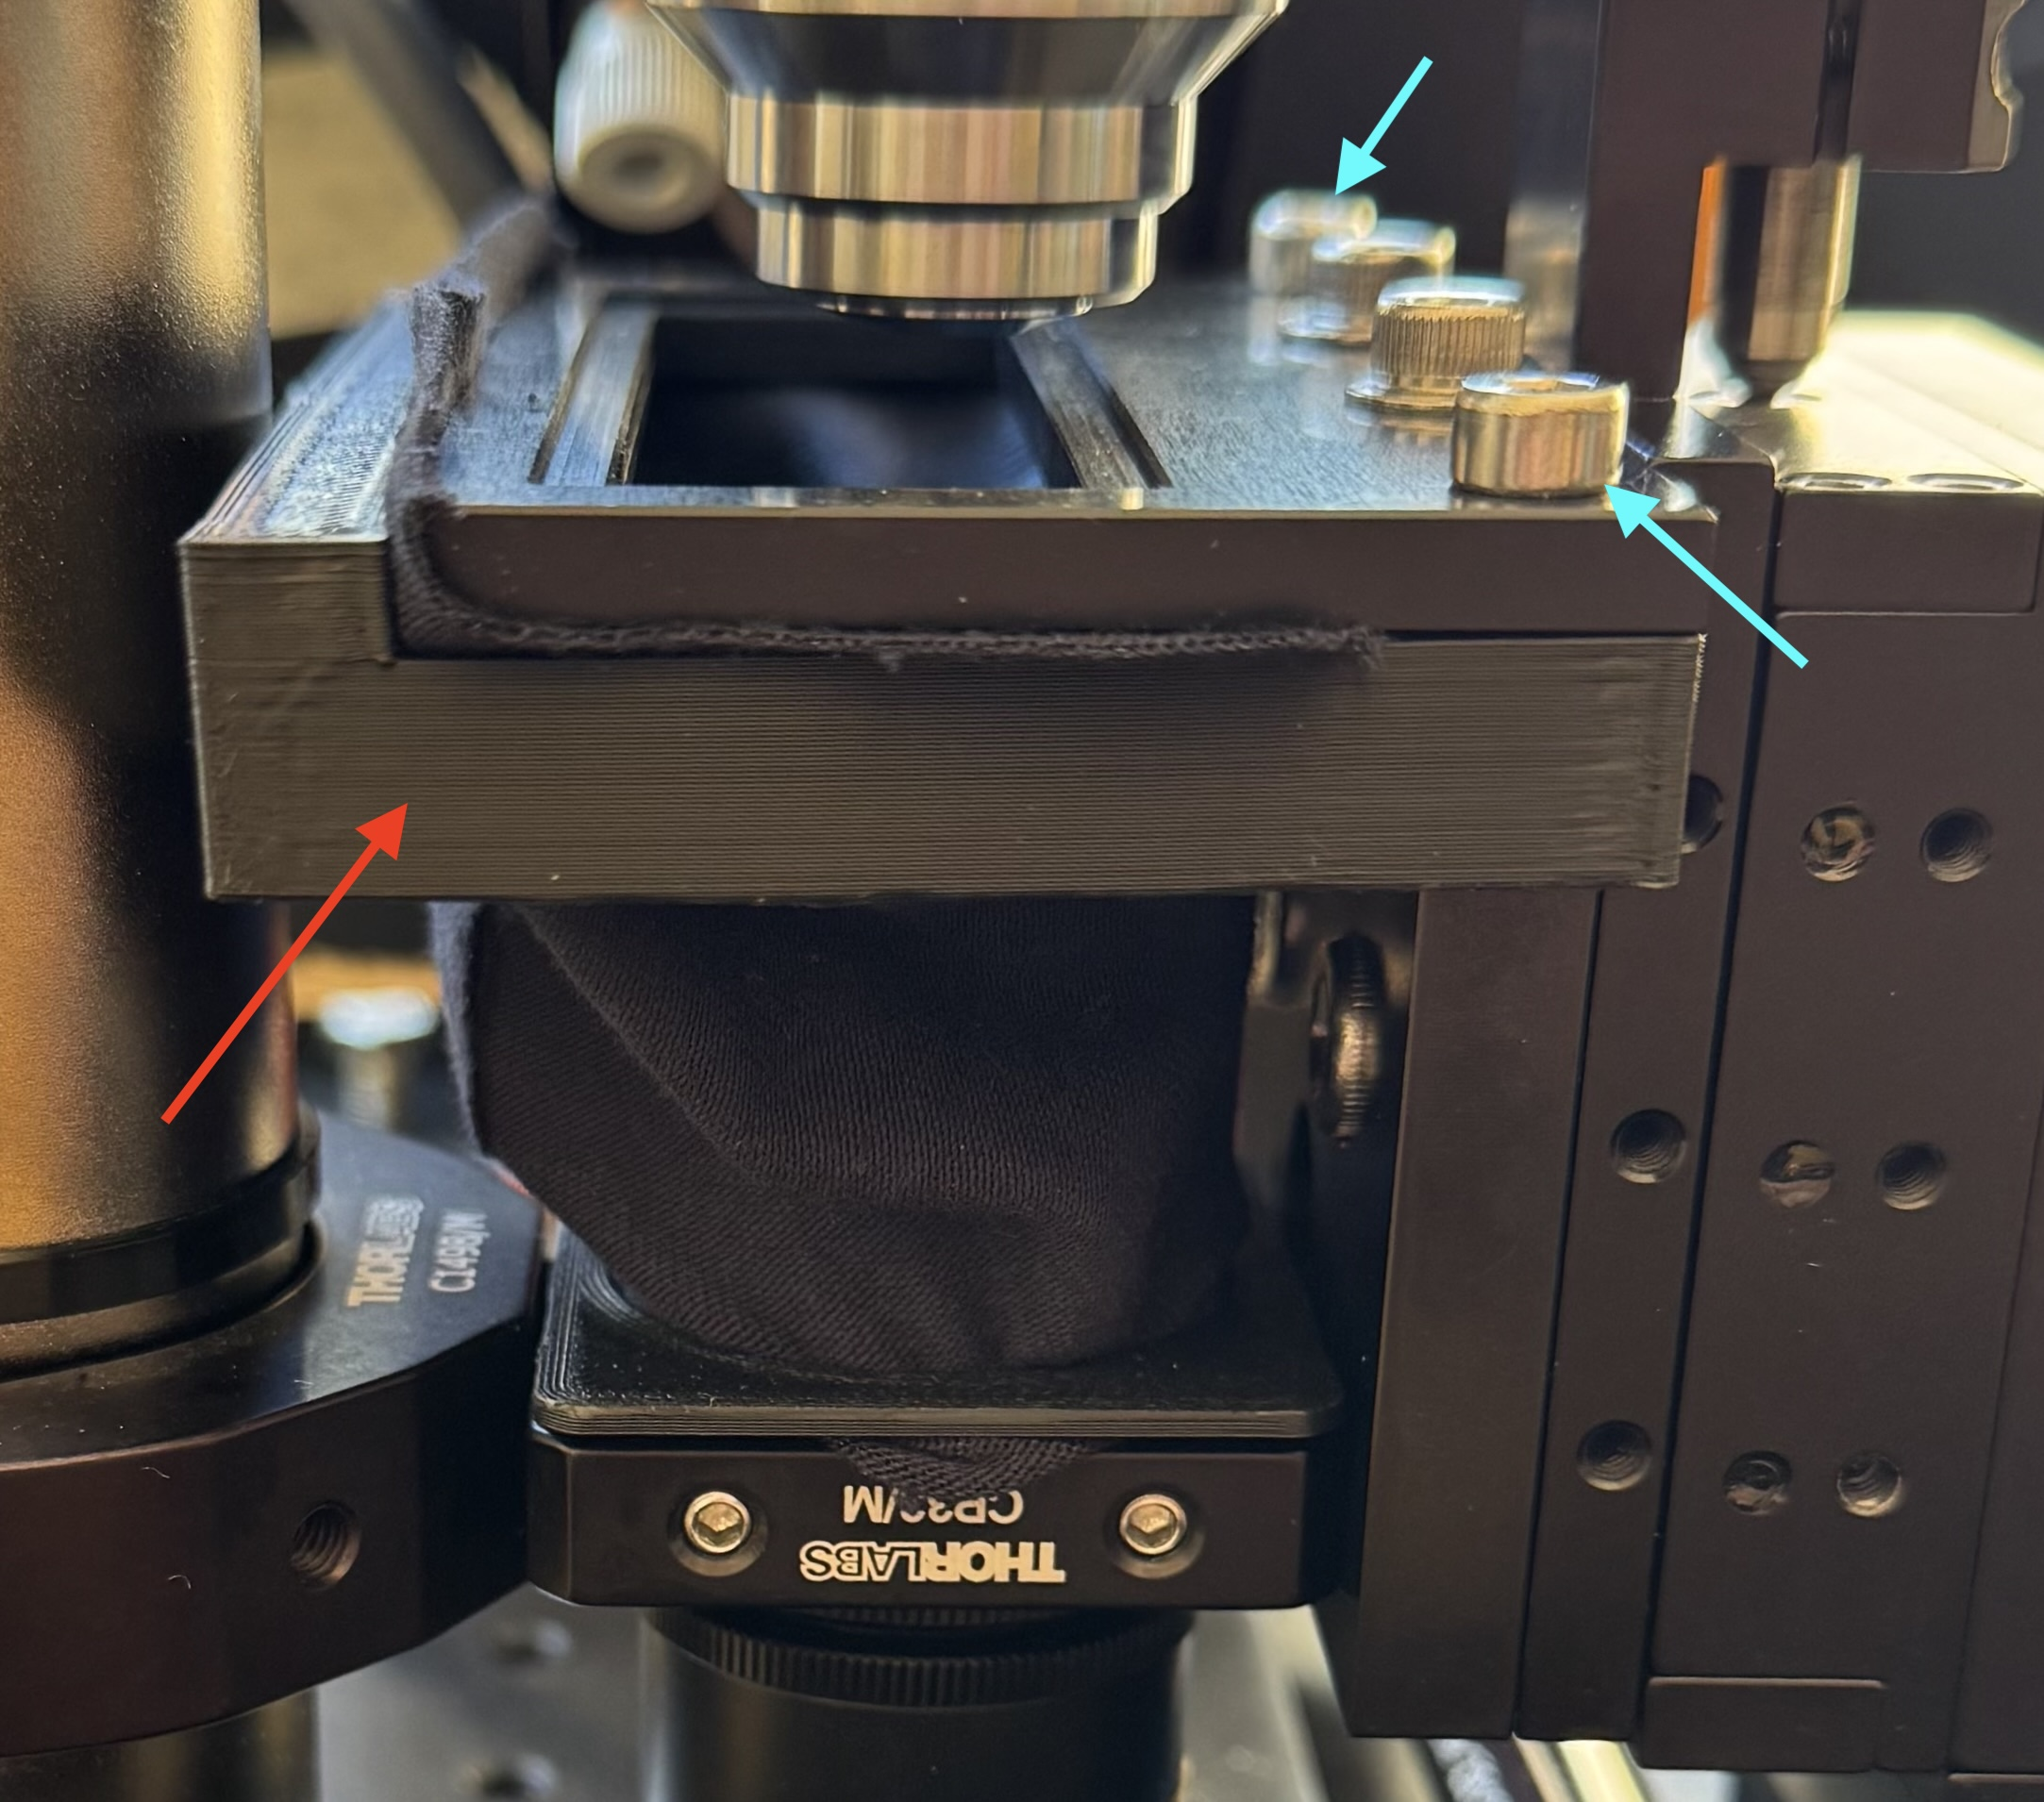
\includegraphics[width=0.9\textwidth]{assets/figures/Protections_laser/Securite_mecanique/Protection_vers_microscope/support_inf_tissu_platine.jpeg}
    \end{center}
    \captionof{figure}{Support pour fixer le tissu inférieur à la platine}
    \label{support_inf_tissu_platine}
\end{minipage}

\subsubsection{Partie supérieure}

\begin{minipage}[c]{0.48\textwidth}
    Pour la partie supérieure, la fixation du tissu est assuré avec le cadre \textcolor[RGB]{233, 173, 56}{jaune} et le support \textcolor[RGB]{170, 50, 50}{rouge} illustré sur la Figure~\ref{model_3D_microscope}. Ce support imprimé est montré par la flèche \textcolor{red}{rouge} sur cette Figure~\ref{support_sup_tissu_microscope} ci-contre.

    \vspace{1em}
    Pour fixer le tissu à la structure au-dessus du microscope, une simple attache rapide (flèche \textcolor[RGB]{115, 210, 210}{bleue}) a été utilisé pour le maintenir en place.

\end{minipage}\hfill
\begin{minipage}[c]{0.48\textwidth}
    \begin{center}
        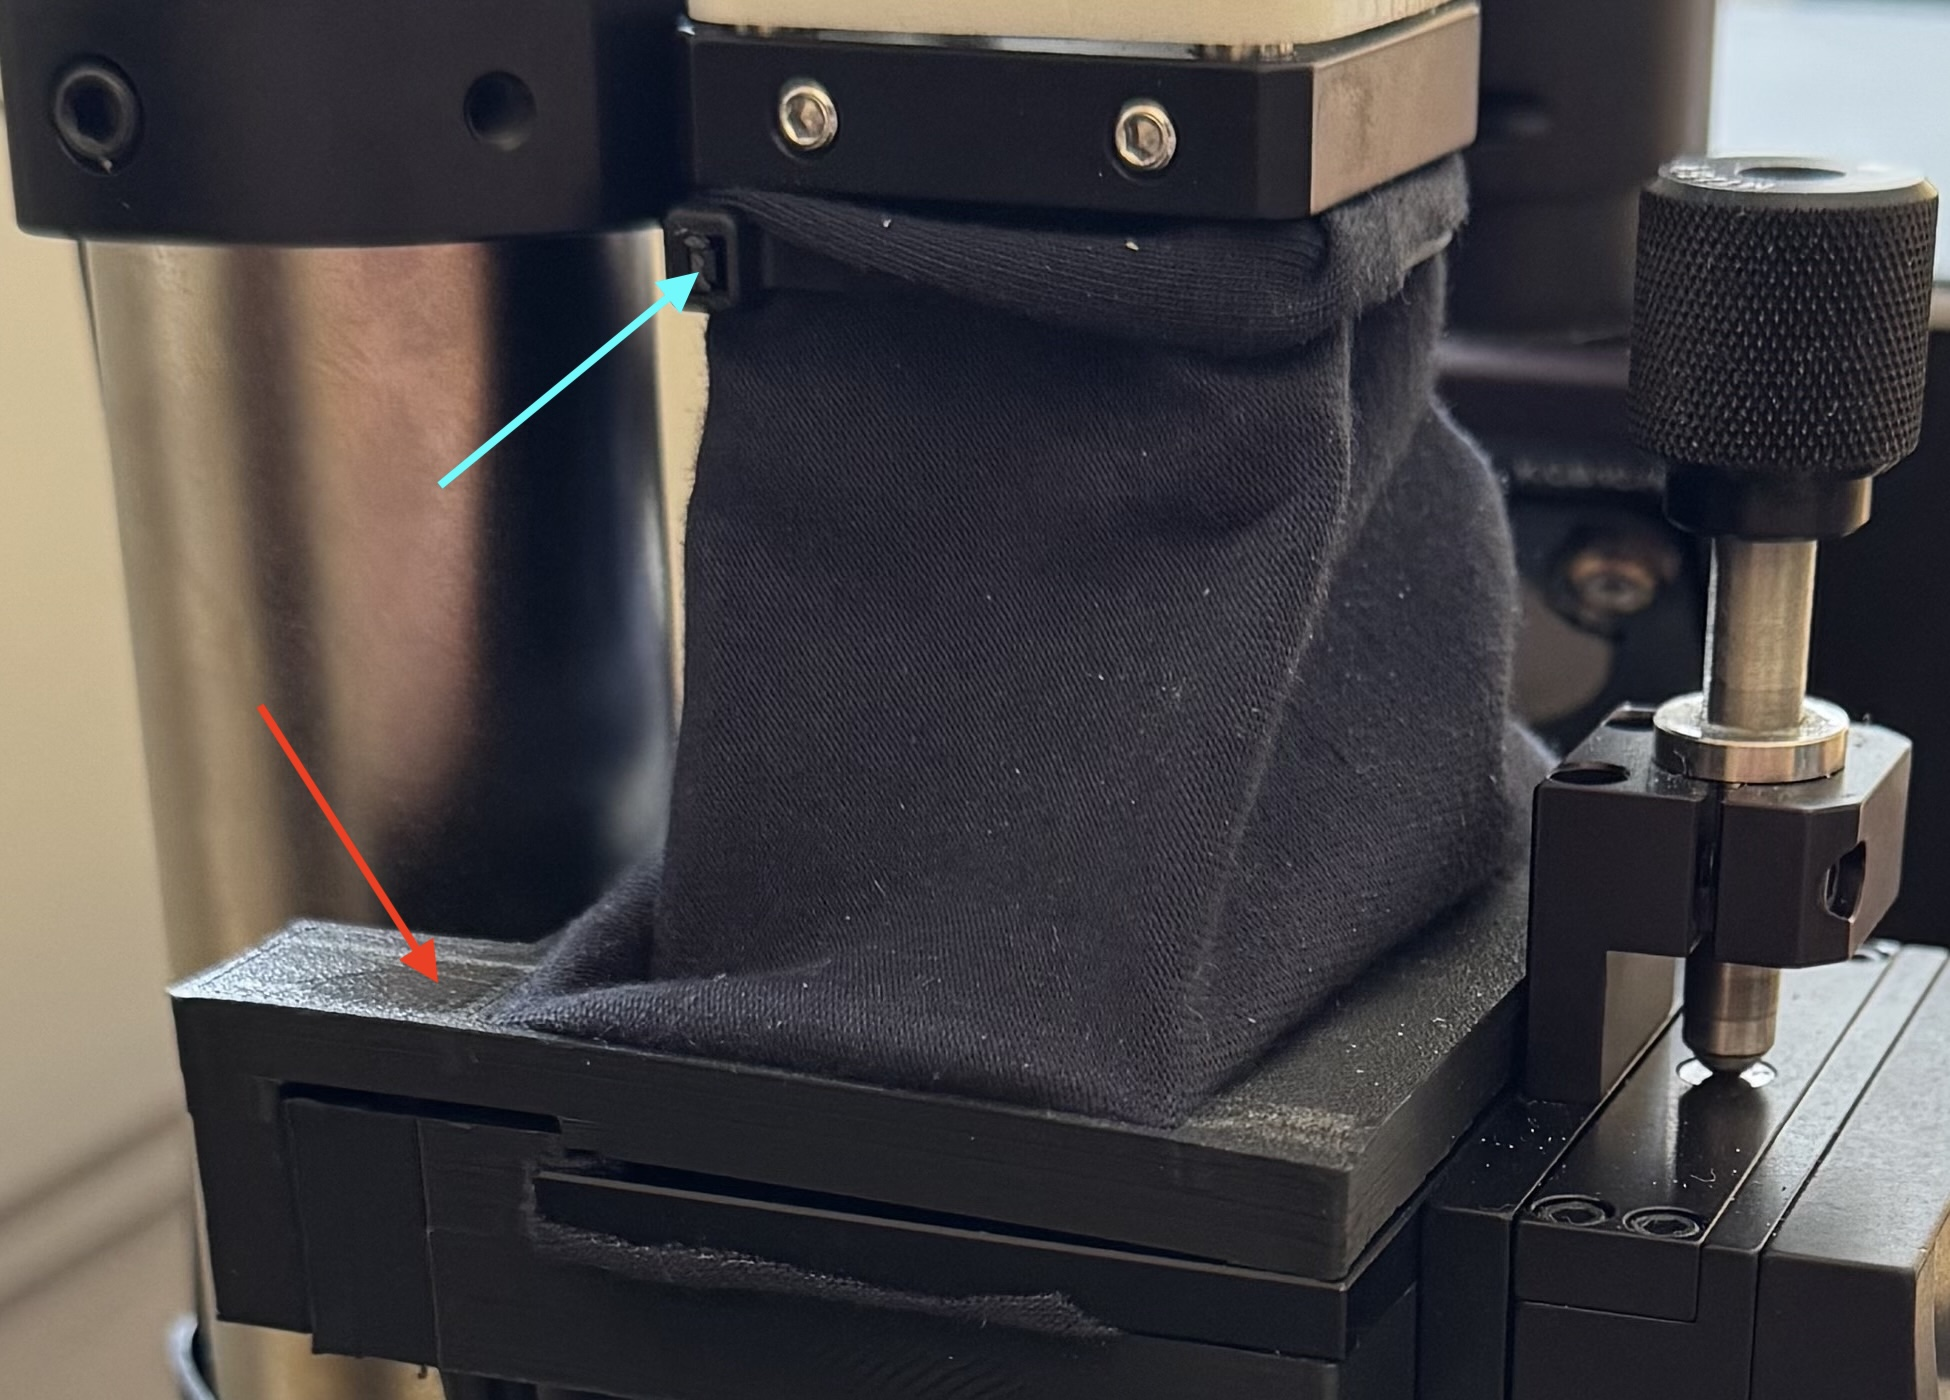
\includegraphics[width=0.9\textwidth]{assets/figures/Protections_laser/Securite_mecanique/Protection_vers_microscope/support_sup_tissu_microscope.jpeg}
    \end{center}
    \captionof{figure}{Support pour fixer le tissu inférieur à la platine}
    \label{support_sup_tissu_microscope}
\end{minipage}

\subsubsection{Fin de course}
\begin{minipage}[c]{0.48\textwidth}
    Afin d'assurer le bon fonctionnement du fin de course, le boîtier modélisé en \textcolor[RGB]{120, 70, 30}{brun} sur la Figure~\ref{model_3D_microscope}, a été créé. Son modèle imprimé est représenté par la flèche \textcolor[RGB]{115, 210, 210}{bleue} sur la Figure~\ref{boitier_fin_de_course}.

    \vspace{1em}
    L'axe, encadré en \textcolor[RGB]{233, 173, 56}{jaune}, assure l'actionnement du fin de course.

\end{minipage}\hfill
\begin{minipage}[c]{0.48\textwidth}
    \begin{center}
        \includegraphics[width=0.9\textwidth]{assets/figures/Protections_laser/Securite_mecanique/Protection_vers_microscope/boitier_fin_de_course.png}
    \end{center}
    \captionof{figure}{Boîtier pour le fin de course}
    \label{boitier_fin_de_course}
\end{minipage}
\chapter{Expérience et notice de laboratoire} \label{chapter:notice_labo}
\section{Expérience pratique avec calcul de force}
Une expérience pratique simple à réaliser avec ce système consiste à mesurer la force de maintien maximale. Cette force correspond à la force maximale que le piège optique peut appliquer pour maintenir une particule dans sa position. L'expérience a été effectuée avec un mélange d'eau distillée et de crème pour les mains (de la marque Nivea), comme proposé dans le manuel d'utilisation fourni par Thorlabs.

Ci-dessous, une liste énumérée expliquant chaque étape avec les calculs nécessaire pour déterminer cette force :

\vspace{1em}
\begin{minipage}{0.6\textwidth}
    \begin{enumerate}
        \item La première étape consiste à connaître le ratio pixels/\textmu m. Pour cela, on mesure une bille de silice dont son diamètre réel est connu : 2,06~\textmu m, et son diamètre dans l'image est de 34 pixels. On obtient donc le ratio suivant :
              \[
                  \text{ratio} = \frac{34~\text{pixels}}{2.06~\text{\textmu m}} = 16,50~\text{pixels/\textmu m}
              \]
        \item On sélectionne ensuite une particule de graisse quelconque et on mesure son diamètre dans l'image (Figure~\ref{mesure_bead}). Cette particule de graisse mesure 136 pixels de diamètre. En utilisant le facteur précédent :
              \[
                  R = \frac{136}{2 \cdot \text{ratio}} = 4,12~\text{\textmu m}
              \]
        \item Toujours avec la même particule, on mesure la vitesse maximale où la particule reste encore piégée par le faisceau laser. Une vitesse maximale de 0,065~mm/s a été mesurée.
    \end{enumerate}
\end{minipage}
\hfill
\begin{minipage}{0.38\textwidth}
    \centering
    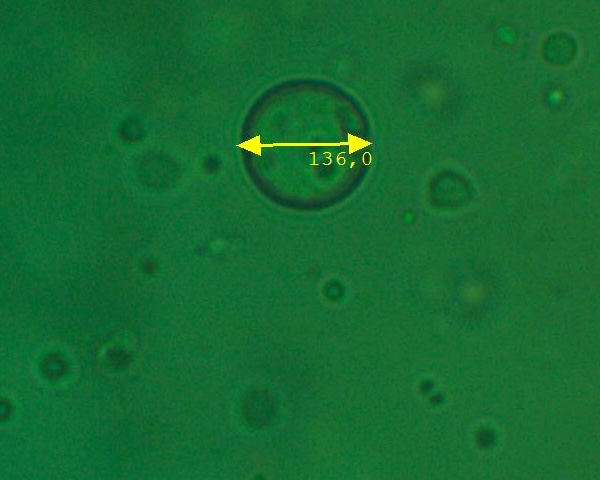
\includegraphics[width=\textwidth]{assets/figures/Notice de laboratoire/mesure_bead.jpg}
    \captionof{figure}{Mesure d'une particule du mélange eau distillée/crème en pixels}
    \label{mesure_bead}
\end{minipage}
\newpage
Une fois toutes ces mesures réalisées, la force de maintien maximale \( F_R \) peut être calculée avec l'équation suivante :
\begin{equation}
    F_R = 6 \pi \eta_{\text{eff}} R v
\end{equation}
\myequations{Force de maintien maximale pour une particule.}
\textbf{Légende :}
\begin{itemize}[label=\textbullet]
    \item $\eta_{\text{eff}}$ : viscosité effective du milieu liquide
    \item $R$ : rayon de la particule
    \item $v$ : vitesse linéaire de la particule dans le liquide
\end{itemize}

\textbf{Calcul numérique :}
\[
    F_R = 6 \pi \cdot 1{,}003 \cdot 10^{-3}~\text{Pa}\cdot\text{s} \cdot 4{,}12 \cdot 10^{-6}~\text{m} \cdot 6{,}5 \cdot 10^{-5}~\text{m/s} = 5{,}06~\text{pN}
\]

\section{Observations avec différents mélanges}
Un mélange d'eau distillée avec du dentifrice au charbon noir (de la marque Primark) a été testé. Sur la figure~\ref{dentifrice_charbon}, on peut apercevoir à ce qui s'apparente à un fragment de charbon noir. Un phénomène surprenant se produit au moment où le laser touche une particule noire : au lieu d'être attirée vers le centre du faisceau laser, elle est repoussée.

\begin{figure}[H]
    \begin{center}
        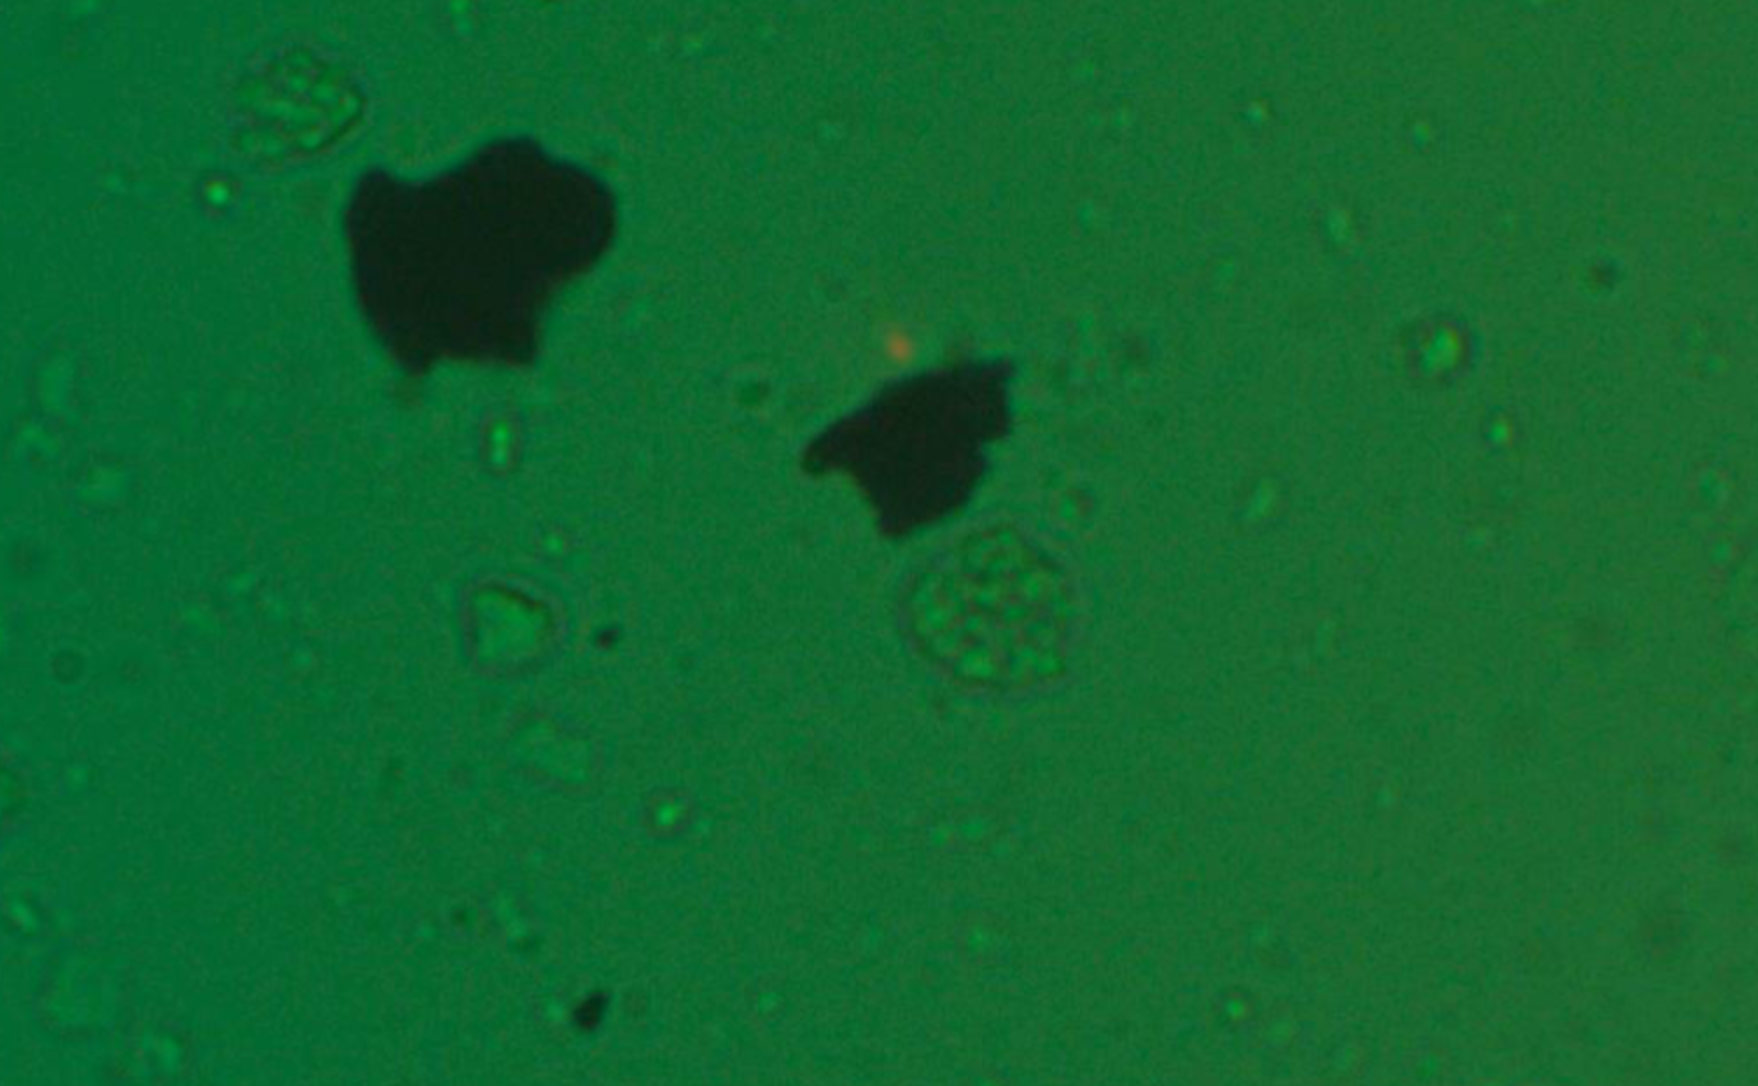
\includegraphics[width=0.7\textwidth]{assets/figures/Notice de laboratoire/dentifrice_charbon.png}
    \end{center}
    \caption{Mélange d'eau distillée avec du dentifrice au charbon noir}
    \label{dentifrice_charbon}
\end{figure}

Ce comportement peut s'expliquer par le fait que la matière noire absorbe fortement la lumière. Contrairement aux particules transparentes qui sont attirées vers le centre du faisceau à cause de la force de gradient, les particules noires, comme le charbon, sont surtout influencées par une force de diffusion. Cette force s'explique par l'absorbtion d'une grande partie de la lumière, par la particule, générant une poussée dans la direction du faisceau. Résultat : au lieu d'être attirée, elle est repoussée par le laser.

\newpage
\section{Contenu de la notice}
Ce système doit pouvoir être exploré par des étudiants lors d'un cours au sein du laboratoire COMATEC-LANS. Comme le manuel d'utilisation du système fourni par Thorlabs comprend 108 pages au total~\cite{manualPortableOpticalTweezers}, il semble nécessaire de concevoir une notice de laboratoire plus compacte, afin de faciliter sa prise en main. La notice complète se trouve en annexes à la page~\pageref{annexe:notice_labo_Kinesis_ThorCam}. Ci-dessous, une liste résumée du contenu de cette notice.

Cette notice de laboratoire est structurée de manière à guider pas à pas l'utilisateur qui souhaite découvrir ce système de pinces optiques.
% La notice est divisée en six parties principales. Elle commence par une présentation détaillée du système et de ses éléments de sécurité. Ensuite, un guide d'installation des logiciels nécessaires (ThorCam et Kinesis) est proposé. La préparation de l'échantillon est expliquée étape par étape, suivie du réglage précis de sa position verticale pour un piégeage efficace. Une partie est ensuite consacrée à la manipulation des particules, accompagnée d'un exemple de calcul de force. Enfin, la dernière section décrit les étapes pour remettre le système en ordre à la fin de l'expérience.
Elle est organisée selon les phases suivantes :

\begin{enumerate}
    \item \textbf{Présentation des composants du système} : description détaillée des éléments constituant le système, avec un intérêt particulier sur les dispositifs de sécurité pour que l'utilisateur puisse facilement les identifier et comprendre leur rôle.

    \item \textbf{Installation et prise en main des logiciels} : guide pas-à-pas pour l'installation des logiciels ThorCam et Kinesis, accompagnée d'une explication claire de leur rôle dans la capture d'image et le contrôle des moteurs.

    \item \textbf{Préparation de l'échantillon} : protocole pour préparer correctement l'échantillon, afin de garantir une manipulation optimale par la pince optique.

    \item \textbf{Réglage précis de la position verticale de l'échantillon} : méthodes pour ajuster la position verticale de la lame dans le système, afin d'optimiser le focus du laser et assurer un piégeage efficace des particules.

    \item \textbf{Expériences de positionnement de particules} : réalisation d'expériences de déplacement des particules à l'aide de la pince optique, avec un calcul détaillé permettant d'estimer la force maximale exercée par le laser pour maintenir les particules piégées.

    \item \textbf{Remise en ordre du système} : Explications pour éteindre, nettoyer et ranger le matériel en fin d'utilisation.
\end{enumerate}

Une notice pour la même expérience, mais en utilisant le logiciel ServoVision est également disponible en annexes à la page~\pageref{annexe:notice_labo_ServoVision}.
\chapter{Développement de l'application ServoVision} \label{chapter:app_servovision}
\section{Introduction}

Le système de Thorlabs doit être utilisé par deux applications distinctes, Kinesis et ThorCam, pour être fonctionnel à 100\%. De ce fait, cela rends son utilisation moins ergonomique. De plus, de nombreuses fonctionnalités ont été implémentées par Thorlabs, aussi bien dans les logiciels Kinesis que ThorCam qui ne sont pas forcément utilisés dans les manipulations. Cela alourdit leur compréhension. Pour une manipulation de laboratoire, il est actuellement nécessaire d'avoir une notice très détaillée pour bien comprendre le fonctionnement du système, installer les logiciels et les configurer. Ce premier point va mener au premier objectif de cette nouvelle application.

Dans l'application Kinesis, aucun système de vision n'est intégrée et de ce fait, il est impossible de détecter automatiquement des particules. Ce second point va mener au deuxième objectif.

\section{Objectifs}
\begin{itemize}[label=\textbullet]
    \item Création de l'application ServoVision qui regroupent les fonctionnalités de base de Kinesis et de ThorCam afin d'avoir qu'une seule application simple d'utilisation. Le nom ServoVision vient de la combinaison de "Servo" pour la gestion des servomoteurs, et "Vision" pour le contrôle de la caméra.
    \item Intégration d'un algorithme pour détecter automatiquement des particules, et de les déplacer de façon autonome.
\end{itemize}

\newpage
\begin{minipage}{\textwidth}
    Ci-dessous, un tableau récapitulatif pour les fonctionnalités reprogrammées dans ServoVision :

    \begin{table}[H]
        \centering
        \begin{tabular}{|p{6cm}|c|c|c|}
            \hline
            \textbf{Fonctionnalité}                        & \textbf{Kinesis} & \textbf{ThorCam} & \textbf{ServoVision} \\
            \hline
            Contrôle des servomoteurs X et Y               & \ding{51}        &                  & \ding{51}            \\
            Contrôle du driver laser                       & \ding{51}        &                  & \ding{51}            \\
            \hline
            Affichage en direct de la caméra               &                  & \ding{51}        & \ding{51}            \\
            Pause / Play du flux caméra                    &                  & \ding{51}        & \ding{51}            \\
            Capture d'image                                &                  & \ding{51}        & \ding{51}            \\
            Enregistrement vidéo                           &                  & \ding{51}        & \ding{51}            \\
            Outils de mesure dans l'image                  &                  & \ding{51}        & \ding{51}            \\
            Zoom caméra                                    &                  & \ding{51}        & \ding{51}            \\
            Navigation caméra                              &                  & \ding{51}        & \ding{51}            \\
            \hline
            {\small Détection automatique de particules}   &                  &                  & \ding{51}            \\
            {\small Déplacement automatique de particules} &                  &                  & \ding{51}            \\
            \hline
        \end{tabular}
        \caption{Fonctionnalités reprogrammées de Kinesis et ThorCam dans l'application ServoVision}
        \label{tab:fonctionnalites_servovision}
    \end{table}
\end{minipage}
\newpage
\section{Choix des solutions}
Thorlabs met à disposition plusieurs outils pour développer sa propre application. Le logiciel Kinesis propose des contrôles .NET utilisables avec des langages comme C\#, Visual Basic, LabVIEW, ou tout autre langage compatible .NET. Des bibliothèques DLL bas niveau sont aussi disponibles. Les langages C, C++ et Python sont également compatible avec le matériel Thorlabs.

Du côté de ThorCam, un SDK (Software Development Kit) est fourni pour développer notre propre interface. Un SDK est un kit fourni par une entreprise qui contient tout le nécessaire (bibliothèques, exemples, docs) pour créer sa propre application. Il est également possible d'utiliser les langages de programmation: C\#, C++, MATLAB et Python.

Grâce à ces bibliothèques et outils, il est donc possible de regrouper les fonctions essentielles de Kinesis et ThorCam dans une seule application personnalisée.
\subsection{Choix du language de programmation}
\begin{table}[H]
    \centering
    \begin{tabular}{|l|c|c|c|c|c|}
        \hline
        \textbf{Critère}                  & \textbf{C\#} & \textbf{C++} & \textbf{Python} & \textbf{MATLAB} & \textbf{LabVIEW} \\
        \hline
        Compatibilité driver moteur       & 6            & 6            & 6               & 6               & 4                \\
        Compatibilité driver laser        & 6            & 6            & 2               & 6               & 2                \\
        Compatibilité caméra              & 6            & 6            & 6               & 6               & 6                \\
        Intégration interface utilisateur & 6            & 4            & 4               & 2               & 2                \\
        Documentation Thorlabs            & 6            & 6            & 4               & 4               & 4                \\
        Facilité de programmation         & 5            & 4            & 5               & 5               & 6                \\
        Multi-plateforme                  & 3            & 5            & 6               & 4               & 4                \\
        Évolutivité                       & 6            & 5            & 5               & 3               & 2                \\
        Modularité                        & 6            & 5            & 5               & 3               & 2                \\
        Organisation du code              & 6            & 5            & 5               & 3               & 2                \\
        \hline
        \textbf{Note moyenne}             & \textbf{5.6} & \textbf{5.2} & \textbf{4.8}    & \textbf{4.2}    & \textbf{3.4}     \\
        \hline
    \end{tabular}
    \caption{Évaluation des langages pour l'application ServoVision (6 = excellent, 1 = faible)}
    \label{tab:langages}
\end{table}
Le tableau~\ref{tab:langages} est composé de critères importants pour l'application. Il en ressort que le C\# est le plus adapté à ce projet. Ce langage permet de créer une interface graphique complète grâce au framework WPF (Windows Presentation Foundation), qui offre une grande flexibilité dans la création d'interfaces modernes. L'organisation claire du code ainsi que sa modularité font de C\# un choix idéal pour une application évolutive et maintenable.

Python est LabVIEW ont obtenu la note de 2 pour la compatibilité avec le driver laser, car Thorlabs n'ont pas d'exemples sur leur github pour cet appareil, mais il faudrait utiliser d'autres librairies supplémentaires~\cite{controlLaserDriverPython}~\cite{controlLaserDriverLabVIEW}.

\newpage
\subsection{Architecture logicielle}
Ci-dessous, le diagramme UML met en évidence les différentes classes principales et leurs relations entre elles.
\begin{figure}[H]
    \centering
    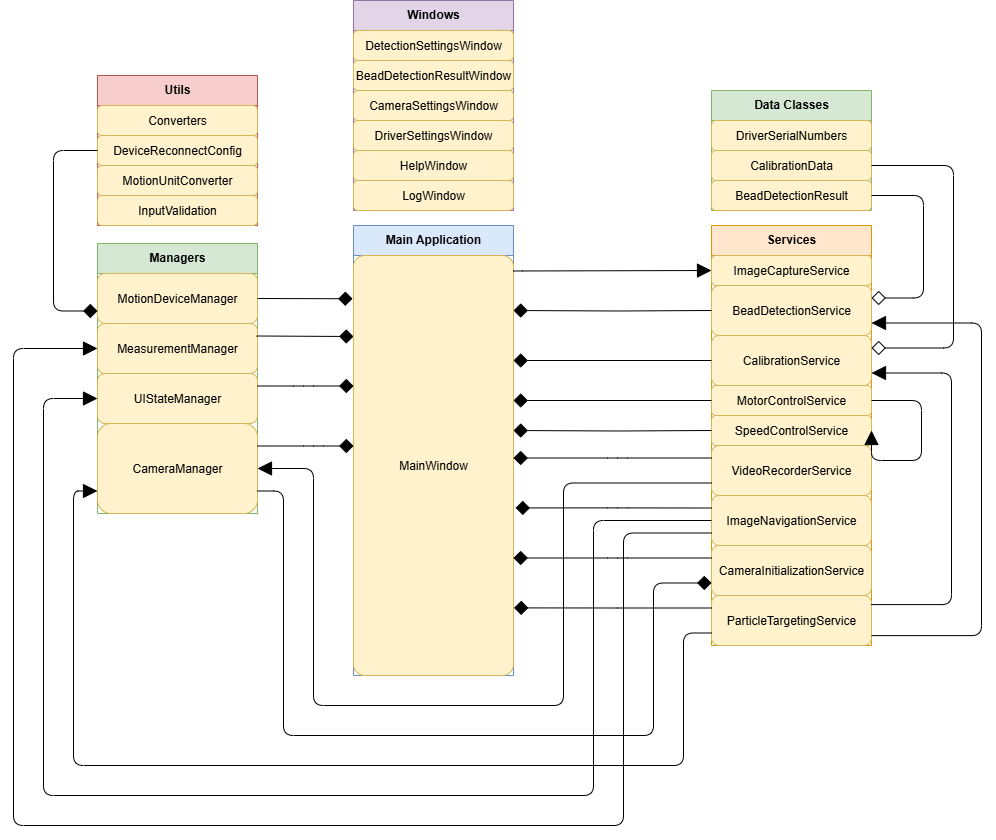
\includegraphics[width=\textwidth]{assets/figures/Application_ServoVision/ServoVision_UML_Diagram.drawio.png}
    \caption{Diagramme UML de l'architecture logicielle de l'application ServoVision}
    \label{uml_servovision}
\end{figure}

Seuls les services sont expliqués ici, car ce sont les principales classes permettant de comprendre le fonctionnement du code. Les différentes fenêtres sont présentées à l'aide de captures d'écran provenant de l'application à la section~\ref{subsection:fenetres}.

\textbf{CalibrationService}
\begin{itemize}[label=\textbullet]
    \item Calibration pour faire correspondre les pas du moteur avec l'image à la caméra
    \item Calcul des facteurs de conversion pixel/mm
\end{itemize}

\textbf{CameraInitializationService}
\begin{itemize}[label=\textbullet]
    \item Détection automatique des caméras Thorlabs
    \item Gestion des erreurs de connexion
\end{itemize}

\textbf{MotorControlService}
\begin{itemize}[label=\textbullet]
    \item Contrôle en temps réel des moteurs X/Y
    \item Contrôle de la vitesse de déplacement
    \item Interface avec le clavier pour les mouvements
\end{itemize}

\textbf{SpeedControlService}
\begin{itemize}[label=\textbullet]
    \item Gestion de la vitesse de déplacement des moteurs
    \item Interface avec les contrôles de vitesse
\end{itemize}

\textbf{ImageNavigationService}
\begin{itemize}[label=\textbullet]
    \item Zoom et dézoom de l'image
    \item Déplacement dans l'image
    \item Gestion des interactions souris
\end{itemize}

\textbf{BeadDetectionService}
\begin{itemize}[label=\textbullet]
    \item Algorithme de détection basé sur OpenCV
    \item Seuillage adaptatif pour avoir une image binaire
    \item Filtrage par taille des objets détectés
\end{itemize}

\textbf{ParticleTargetingService}
\begin{itemize}[label=\textbullet]
    \item Sélection de particules par clic
    \item Calcul des mouvements moteur nécessaires
    \item Compensation du jeu mécanique
    \item Mouvement automatique vers la particule sélectionnée
\end{itemize}

\textbf{ImageCaptureService}
\begin{itemize}[label=\textbullet]
    \item Capture d'images individuelles
    \item Organisation des fichiers par date/heure
    \item Interface utilisateur pour la sélection du dossier
\end{itemize}

\textbf{VideoRecorderService}
\begin{itemize}[label=\textbullet]
    \item Enregistrement vidéo en temps réel
    \item Sauvegarde automatique des vidéos
\end{itemize}

\newpage
\subsection{Présentation de l'application} \label{subsection:fenetres}
\subsubsection{Moteurs X / Y, Laser et calibration}

\begin{figure}[H]
    \centering
    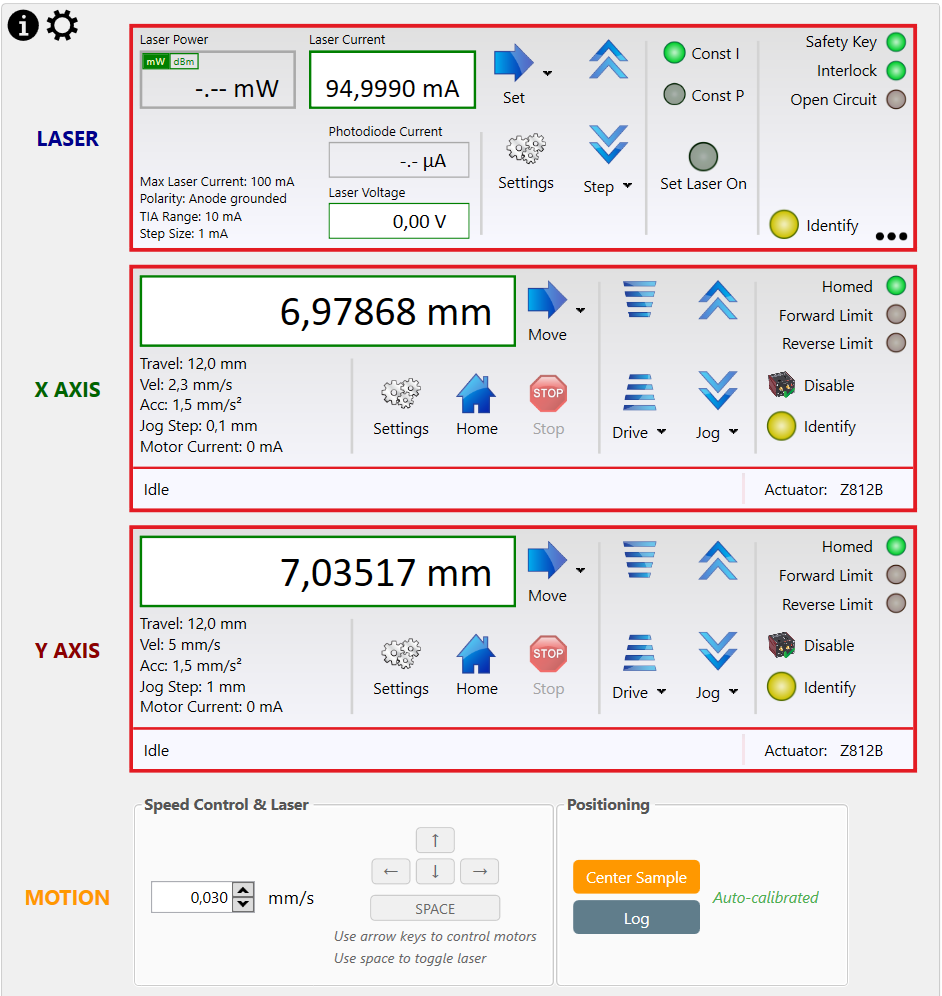
\includegraphics[width=\textwidth]{assets/figures/Application_ServoVision/Moteurs_Laser_Calibration.png}
    \caption{Interface de contrôle des moteurs, du laser et de la calibration}
    \label{Moteurs_Laser_Calibration}
\end{figure}
Cette partie de l'application permet de gérer les moteurs, le laser et la calibration. On peut voir que les trois drivers reprennent exactement le même visuel que dans Kinesis. La bibliothèque fournie par Thorlabs permet d'intégrer directement leurs modules dans une application personnalisée. C'est un point positif, car je n'ai pas eu à reprogrammer tous les boutons de ces drivers.

Dans l'onglet \textcolor[RGB]{241,158,56}{\textbf{MOTION}} il y'a deux sous-groupes, le premier est \textbf{Speed Control \& Laser}, il permet de choisir la vitesse en mm/s souhaitée, puis il suffit d'utiliser les touches du clavier pour se déplacer. Pour un confort optimal, l'appui sur la touche espace permet d'activer/désactiver le laser.

\newpage
Dans le deuxième sous-groupe \textbf{Positioning}, on retrouve le premier bouton \textcolor[RGB]{241,158,56}{\textbf{Center Sample}} qui permet de centrer l'échantillon sous le microscope, ce qui correspond à un déplacement des axes X et Y à 7mm sur chacun d'eux.

Le bouton \textcolor[RGB]{102,125,138}{\textbf{Log}} affiche les logs de la calibration~(Figure~\ref{Calibration_Center_logs}).
\begin{figure}[H]
    \centering
    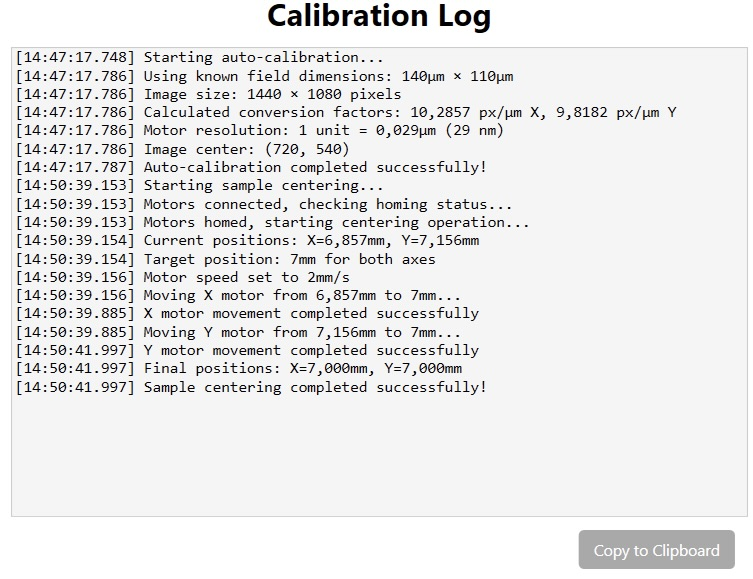
\includegraphics[width=0.8\textwidth]{assets/figures/Application_ServoVision/Calibration_Center_logs.jpeg}
    \caption{Calibration avec sa journalisation}
    \label{Calibration_Center_logs}
\end{figure}
Cette calibration consiste à calculer combien il y a de pixels pour 1~\textmu m dans l'image de la caméra, pour ensuite savoir de combien doit se déplacer un moteur pour parcourir une certaine distance en unité réelle.

Pour connaître la taille du champ observé, je place un point fixe sur un bord de l'image, puise je me déplace jusqu'à ce que ce même point soit de l'autre côté. Je peux ensuite observer l'écart affiché par le servomoteur. Je fais la même procédure pour l'autre dimension.

Connaissant la résolution de l'image capturée par la caméra et la taille du champ observé en \textmu m, on peut calculer un facteur de conversion en X et en Y.

Dans notre cas:
\begin{itemize}
    \item Image : 1440~$\times$~1080 pixels (section 5.1 du manuel de la caméra~\cite{cameraCS165CU/M})
    \item Champ de la caméra : 140~\textmu m~$\times$~110~\textmu m
\end{itemize}

Les équations des facteurs de calibration en X et Y sont :

\[
    \text{Facteur}_X = \frac{1440\ \text{pixels}}{140\ \mu m} = 10.29\ \text{pixels}/\mu m
\]
\[
    \text{Facteur}_Y = \frac{1080\ \text{pixels}}{110\ \mu m} = 9.82\ \text{pixels}/\mu m
\]

On connaît aussi le pas des moteurs de la table du microscope utilisé : 1~pas~=~29~nm (section 5.2 du manuel des moteurs~\cite{motorZ812B}). Grâce à ça, on peut directement relier un déplacement moteur à une distance réelle. À l'aide des facteurs de calibration pixels/\textmu m, ça permet un positionnement précis basé sur l'image de la caméra.

\subsubsection{Réglage numéros de série des drivers}

\begin{minipage}[c]{0.4\textwidth}
    En cliquant sur la roue dentée en haut à gauche (Figure~\ref{Moteurs_Laser_Calibration}), il est possible de modifier les numéros de séries de chaque driver. La connexion de nouveaux appareils se fait automatiquement. Un bouton reset est présent afin de remettre les numéros de séries par défaut des appareils. Ces numéros sont montrés dans la figure~\ref{Settings_Drivers}.
\end{minipage}
\begin{minipage}[c]{0.58\textwidth}
    \begin{center}
        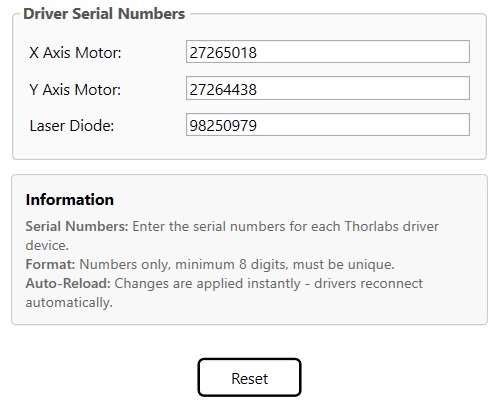
\includegraphics[width=\textwidth]{assets/figures/Application_ServoVision/Settings_Drivers.png}
    \end{center}
    \captionof{figure}{Configuration des numéros de série des drivers}
    \label{Settings_Drivers}
\end{minipage}

\subsubsection{Caméra, outil de mesure, capture d'écran}

\begin{figure}[H]
    \centering
    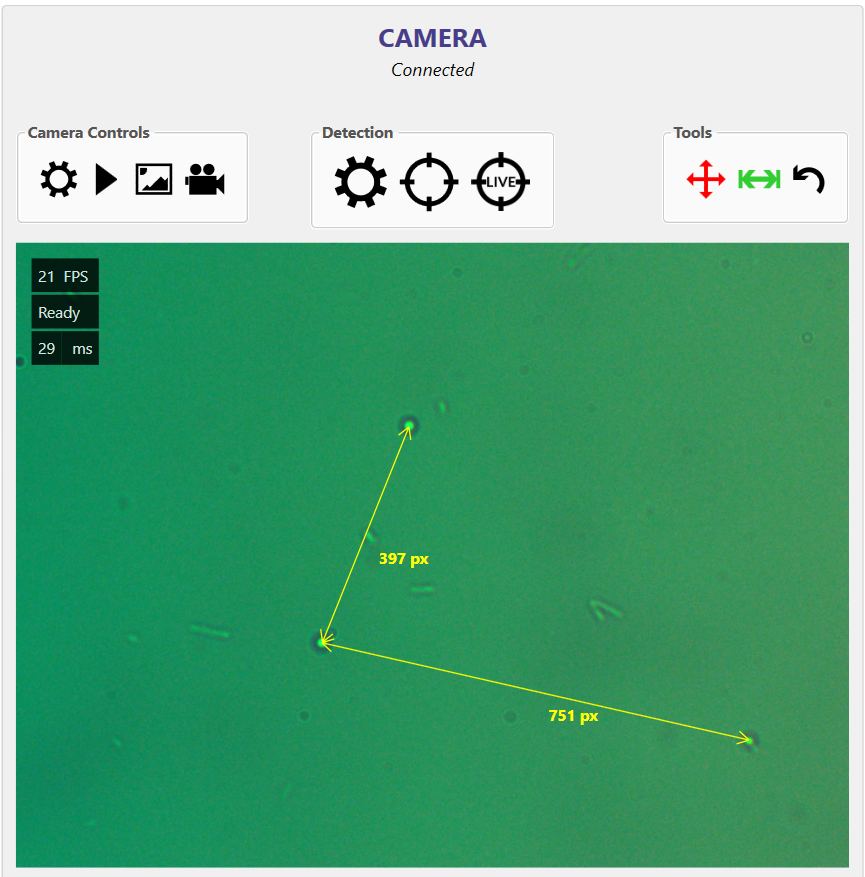
\includegraphics[width=0.7\textwidth]{assets/figures/Application_ServoVision/Measure_Tool.png}
    \caption{Interface de contrôle de la caméra}
    \label{Measure_Tool}
\end{figure}
La partie de droite de l'application concerne l'interface de la caméra. Au centre de l'image, on aperçoit le retour visuel de la caméra. Deux sous-groupes vont être détaillés ici.
\newpage
Le premier sous-groupe \textbf{Camera Controls}, permet la gestion visuelle de l'image, on y retrouve :
\begin{itemize}[label=\textbullet]
    \item Le bouton \textbf{PLAY} met en pause l'image.
    \item Le bouton avec une \textbf{image de paysage} permet de faire une capture d'écran de l'image en cours.
    \item Le bouton \textbf{Camera} enregistre une vidéo de l'image en cours.
    \item
          \begin{minipage}{0.4\textwidth}
              Le bouton \textbf{Réglages} ouvre les paramètres de la caméra (Figure~\ref{Settings_Camera}) où l'on va pouvoir modifier les gains de couleurs sur le rouge, vert et bleu. Le temps d'exposition est également un paramètre qui peut être réglé.
          \end{minipage}
          \hfill
          \begin{minipage}{0.55\textwidth}
              \centering
              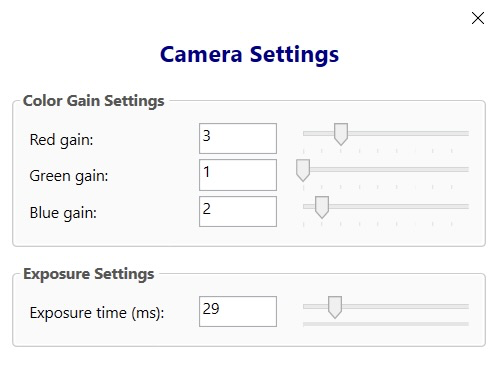
\includegraphics[width=\textwidth]{assets/figures/Application_ServoVision/Settings_Camera.png}
              \captionof{figure}{Réglages de la caméra}
              \label{Settings_Camera}
          \end{minipage}
\end{itemize}
Le sous-groupe \textbf{Tools} contient trois boutons :
\begin{itemize}[label=\textbullet]
    \item La première fonctionnalité qui n'est pas représentée par un bouton est le zoom. Avec la molette de la souris, il est possible de zoomer et de dézoomer dans l'image.
    \item Le premier bouton représenté par quatres flèches permet de se déplacer dans l'image une fois zoomé à l'intérieur.
    \item Le deuxième bouton, avec deux flèches, est un outil de mesure. Il permet de mesurer en pixels la distance entre deux points de l'image. Lors de l'affichage, des flèches jaunes sont dessinées avec la dimension en pixels indiquée à côté (Figure~\ref{Measure_Tool}).
    \item Le dernier bouton avec une flèche incurvée permet de supprimer la dernière flèche dessinée.
\end{itemize}

\newpage
\subsubsection{Détection automatique de particules avec adaptative threshold}
Le dernier sous-groupe \textbf{Detection} va regrouper toutes les fonctionnalités par rapport à la détection de particules. Le premier bouton \textbf{Réglage} va être détaillé avec la Figure~\ref{Settings_Detection}.
\begin{figure}[H]
    \centering
    \includegraphics[width=0.9\textwidth]{assets/figures/Application_ServoVision/Settings_Detection.jpeg}
    \caption{Réglages de la détection des particules, les particules numérotées sont celles détectées par l'algorithme}
    \label{Settings_Detection}
\end{figure}
Le premier sous-groupe, \textbf{Particle Detection Settings}, permet de gérer les différents paramètres pour la détection de particules.

L'algorithme principal utilisé pour cette détection est l'\textit{adaptive threshold} de la bibliothèque OpenCV. L'adaptive thresholding calcule un seuil différent pour chaque pixel en fonction de l'intensité locale dans une région définie par le paramètre  \textit{block size} (taille du voisinage). Le seuil est ajusté en soustrayant une valeur constante appelée \textit{offset}, ce qui permet d'affiner la sensibilité du seuillage~\cite{OpenCVadaptativeThreshold}.
\newpage
\begin{figure}[H]
    \centering
    \includegraphics[width=0.9\textwidth]{assets/figures/Application_ServoVision/Settings_Detection_zoom.png}
    \caption{Zoom sur l'image noir et blanc \textit{Binary Adaptive Threshold} de la figure~\ref{Settings_Detection}}
    \label{Settings_Camera_zoom}
\end{figure}

L'algorithme fonctionne seulement si un anneau de pixels éteints (noirs) est fermé. On peut voir sur la figure~\ref{Settings_Camera_zoom}, l'anneau noir à droite sera considéré comme une particule, et à gauche non car ce n'est pas fermé.

Au moment de dire si oui ou non une zone de l'image est considérée comme une particule, la plus grande zone de pixels allumés (blancs) est retirée, car elle correspond au fond blanc de l'image. Découlant de cette opération, si un anneau de pixels éteint n'est pas complétement fermé, il sera intégré à cette grande forme et ne sera pas identifié comme une vraie particule.

Ensuite, il suffit d'énumérer les zones blanches restantes (donc l'intérieur des anneaux noirs fermés) qui sont des particules.

On peut définir l'aire minimale et maximale, en pixels, qu'une région blanche doit avoir pour être considérée comme une particule.

Une série d'images tests est disponible à l'utilisateur pour qu'il puisse essayer différents paramètres.

Toujours dans le sous-groupe \textbf{Detection}, le bouton au milieu avec une \textbf{cible}, lance une détection de particules sur une image capturée. Le même bouton, mais avec le mot \textbf{LIVE} en son centre, lance également une détection de particules, mais cette fois en temps réel.
\newpage
\begin{figure}[H]
    \centering
    \includegraphics[width=\textwidth]{assets/figures/Application_ServoVision/Live_Targeting_Bead.png}
    \caption{Détection de particules en temps réel}
    \label{Live_Targeting_Bead}
\end{figure}

Dans le sous-groupe \textbf{Detected Particles} de la Figure~\ref{Live_Targeting_Bead}, il est possible de visualiser la liste des particules détectées, avec leur coordonnées et un numéro attribué à chacune d'elles. Les coordonnées en X se lisent de gauche à droite, et pour celles en Y de haut en bas.

\newpage
\subsubsection{Déplacement automatique de particules vers le laser}
Une dernière fonctionnalité au niveau de déplacement automatique de particules a été ajoutée. Si le système détecte une particule, l'utilisateur peut cliquer sur celle-ci dans la liste, et le système va amener cette particule choisie aux coordonnées du laser.

Comme première approche, on pourrait penser qu'il suffit de prendre les coordonnées de la particule sélectionnée, puis de déplacer les moteurs pour aligner le laser sur celle-ci. En réalité, c'est plus complexe que cela.

Un paramètre qui paraît anodin, mais qui a toute son importance à cette échelle, est le \textbf{jeu mécanique des moteurs}. En effet, lorsqu'on effectue un déplacement dans une direction, puis qu'on veuille repartir dans la direction opposée, il faut d'abord compenser ce jeu.

Pour les moteurs utilisés dans ce système (Z812B), la datasheet indique qu'il y a un jeu mécanique (\textit{backlash}) inférieur à 8~\textmu m (section 5.1 de la datasheet~\cite{motorZ812B}).

La procédure du déplacement de la particule sous le laser est décrite ci-dessous:
\begin{enumerate}
    \item Mouvements en X et Y de +8~\textmu m pour être sûr de corriger le jeu mécanique.
    \item Une nouvelle image est acquise et on cherche la particule la plus proche de la particule trouvée avant les déplacements, ce qui devrait donner la même particule, en supposant qu'elle n'a pas bougée. À présent, les vraies coordonnées de la particule sont acquises.
    \item Calcul de la distance à parcourir entre la particule et le laser.
    \item Déplacement vers le laser en X et en Y.
    \item
          La dernière étape consiste à rattraper une dernière fois le jeu mécanique. La Figure~\ref{schema_explicatif_jeu} illustre ce problème. Pour amener le laser sur la particule, appliquer simplement un déplacement en X et en Y ne suffit pas :  quatres cas différents risquent d'arriver.

          Si la particule se trouve dans le quadrant n\textsuperscript{o}1, le positionnement final sera juste. En revanche, si elle se situe dans un autre quadrant, il reste une dernière opération à effectuer.

          Vu que la compensation du jeu mécanique a été effectué dans les directions positives de chaque axe, un déplacement dans la direction opposée nécessitera de compenser à nouveau le jeu.

\end{enumerate}
\begin{figure}[H]
    \centering
    \includegraphics[width=0.9\textwidth]{assets/figures/Application_ServoVision/Schema_explicatif_jeu_mecanique.jpeg}
    \caption{Schéma explicatif pour la compensation du jeu mécanique des moteurs}
    \label{schema_explicatif_jeu}
\end{figure}

\subsubsection{Fiabilité et répétabilité de la détection et déplacement d'une particule}
\textbf{Fiabilité}

La fiabilité de la détection dépend pas mal des bons réglages à faire dans les paramètres (taille des particules, seuils, etc...). Si on prend le temps de bien les ajuster pour les conditions d'image qu'on a (bon contraste, particules bien visibles), la détection fonctionne bien. Une fois les bons paramètres trouvés, la particule est détectée presque à chaque fois, ce qui montre que la fiabilité est plutôt bonne.

\textbf{Répétabilité}

Tant que la position de la particule est bien connue et que la connexion avec les moteurs fonctionne, le déplacement jusqu'au laser se fait sans problème. Le système refait les mouvements de manière stable. Bien sûr, il peut y avoir un léger décalage à l'arrivée. Le plus gros écart que j'ai pu observer était d'environ 20 pixels.

En résumé, le système est fiable tant au niveau de la détection que du déplacement, à condition de bien régler les paramètres de base. Ça fonctionne bien dans la majorité des cas, avec une précision qui reste suffisante pour l'objectif visé.

\chapter{Conclusion}
%%if
% Bien que non nécessaire dans un rapport de Bachelor, la discussion finale d'un projet résume les résultats obtenus et dresse une conclusion objective du projet. Un manager de société est souvent amené à lire de nombreux rapport, il ne s'intéresse généralement qu'à l'introduction au contexte de l'étude et à sa conclusion.

% Si nécessaire, n'hésitez pas à scinder votre conclusion en deux parties : une conclusion technique et une conclusion personnelle.

% Il est de coutume de signer la conclusion...
%%fi
\section*{Bilan technique}
Depuis la réception du système de pinces optiques au début du travail de bachelor, de nombreuses améliorations ont pu être réalisées.

\textbf{Sécurité} :
Le système a été optimisé pour éviter tout contact direct avec le laser. Deux protections mécaniques associées chacune à un capteur électrique ont été confectionnées afin de garantir une utilisation sécurisée du système sans protection contre le laser. La première protection, située proche du laser, est un assemblage de trois tôles en aluminium accompagné d'une charnière industrielle. Celle-ci intègre un capteur qui, lorsque la protection est ouverte, coupe l'alimentation du laser. La seconde protection, située autour du microscope et imprimée en 3D, est complétée par un capteur de fin de course qui, lui aussi, coupe le laser à la moindre ouverture. Comme dans toute installation mécano-électrique, un arrêt d'urgence a été câblé, désactivant le faisceau laser. Le système correspond ainsi à un système de classe 1, lorsqu'il est fermé. Seulement l'ajustement du chemin optique nécessite l'utilisation des lunettes de protection (en mode maintenance), c.f. chapitre~\ref{section:maintenance}.

\textbf{Ergonomie} :
Une amélioration a été faite au niveau du câblage des alimentations et des câbles de communication. Le système nécessite quatre connexions USB-A pour communiquer avec l'ordinateur. Un hub USB-A à 4 ports a donc été intégré pour que finalement, un seul câble USB-A soit à brancher sur le poste. Un bouton à clé a aussi été câblé pour pouvoir manipuler le laser plus facilement lors de la maintenance, même lorsque les protections sont ouvertes.

\textbf{Application ServoVision} :
Cette application en C\#, utilisant WPF, a été programmée en regroupant les fonctionnalités de Kinesis ainsi que de ThorCam pour faciliter l'utilisation du système. Un algorithme détectant automatiquement des particules a été implémenté. Il est également possible de déplacer automatiquement une particule sous le laser.

\textbf{Notice de laboratoire} :
Le manuel d'utilisation fourni par Thorlabs étant volumineux, une notice de laboratoire a été écrite pour une prise en main rapide du système.

\textbf{Expériences de force d'attraction de particule} :
Plusieurs expériences ont été menées avec différentes matières. Le calcul de la force de maintien maximale d'une particule de graisse avec un mélange d'eau distillée et de crème a été réalisé.

\section*{Conclusion personnelle}
Ce travail de bachelor a fait appel à plusieurs domaines : la conception mécanique pour les protections, l'électricité et le câblage pour les différents capteurs ainsi que les boutons, et la programmation de l'interface homme-machine pour l'application ServoVision. Personnellement, j'aime quand le travail que j'entreprends est varié. De mon point de vue, les objectifs ont été atteints. Le système est fonctionnel, sécurisé pour des utilisateur\(\cdot\)trices non-expert\(\cdot\)es, et comporte une application ergonomique facile d'utilisation.
\vfil
\hspace{8cm}\makeatletter\@author\makeatother\par
\hspace{8cm}\begin{minipage}{5cm}
    %%if
    % Place pour signature numérique
    \printsignature
    %%fi
\end{minipage}

%% Remerciements
\chapter*{Remerciements}
\addcontentsline{toc}{chapter}{Remerciements}
Je tiens à remercier toutes les personnes qui m'ont aidé tout au long de ce projet de bachelor.

Un grand merci à ma copine, Cloé Allard, pour sa relecture du rapport.

Je remercie également les étudiants du cours de NANO qui ont pu tester la première version de ma notice de laboratoire. Leurs retours m'ont permis d'apporter les modifications nécessaires pour améliorer le document.

Merci aussi à ma professeure, Mme Schintke, pour son accompagnement tout au long du projet, ainsi qu'a M. Del Rossi pour son aide technique et ses conseils.

%% Sommaire et tables
\clearemptydoublepage
{
    \listoffigures
    \let\cleardoublepage\clearpage
    \listoftables
    \let\cleardoublepage\clearpage
    \listofmyequations
    \let\cleardoublepage\clearpage
    % \listoflistings % Liste des codes sources
}

\clearpage
\printbibliography
\appendix
\appendixpage
\addappheadtotoc \label{chapter:annexes}

%%if
% \chapter{Première annexe} \label{chapter:annexes}
Les annexes contiennent généralement :

\begin{itemize}
    \item les dessins mécaniques (mises en plan);
    \item les schémas électriques détaillés;
    \item des photographies du projet;
    \item des scripts et des extraits de code source;
    \item des documents techniques \pex \emph{datasheet};
    \item des développements mathématiques.
\end{itemize}

\section{Mise en plan des trois protections à l'entrée du laser}
\begin{figure}[H]
    \centering
    \includegraphics[angle=90,width=\textwidth]{assets/figures/Annexes/Mises_en_plan/mise_en_plan_avant.png}
    \caption{Mise en plan du capot inférieur avant}
    \label{mise_en_plan_capot_avant}
\end{figure}

\begin{figure}[H]
    \centering
    \includegraphics[angle=90,width=\textwidth]{assets/figures/Annexes/Mises_en_plan/mise_en_plan_arriere.png}
    \caption{Mise en plan du capot inférieur arrière}
    \label{mise_en_plan_capot_arriere}
\end{figure}

\begin{figure}[H]
    \centering
    \includegraphics[angle=90,width=\textwidth]{assets/figures/Annexes/Mises_en_plan/mise_en_plan_superieur.png}
    \caption{Mise en plan du capot supérieur}
    \label{mise_en_plan_capot_superieur}
\end{figure}
%%fi

\let\cleardoublepage\clearpage
\backmatter

\label{glossaire}
\printnoidxglossary
\label{index}
\printindex

% Le colophon est le dernier élément d'un document qui contient des notes de l'auteur concernant la mise en page et l'édition du document : il est parfaitement optionnel.
%%if
\clearpage
\Large\textbf{Colophon :}\par\normalsize
\thispagestyle{empty}
La qualité de cet ouvrage repose que le moteur \LaTeX. La mise en page et le format sont inspirés d'ouvrages scientifiques tels que le modèle de thèse de l'EPFL et celui des publications O'Reilly.

Les mises en plan et les représentations 3D sont exportées de Autodesk Fusion 360.

% Les diagrammes et les illustrations sont édités depuis l'outil en ligne draw.io. Certaines illustrations ont été reprises dans Adobe Illustrator. Les représentations 3D sont exportées de SolidWorks et certains graphiques sont générés à la volée depuis un code source Python.

% L'auteur fictive de ce document \emph{Maria Bernasconi} est un nom emprunté, par amusement, aux spécimens publiés par Postfinance.

Ce document a été compilé avec XeLaTeX.

La famille de police de caractères utilisée est \emph{Computed Modern} créée par Donald Knuth avec son logiciel METAFONT.
\vfil
% Le Colophon est le dernier élément d'un document qui contient des notes de l'auteur concernant la mise en page et l'édition du document : il est parfaitement optionnel.
%%fi

\end{document}
